\documentclass[oneside,a4paper,12pt]{book}
\usepackage{subcaption}
\usepackage[lmargin=2.8cm, rmargin=2.8cm, tmargin=3.3cm, bmargin=3.3cm]{geometry}
\linespread{1.1}
\setlength{\parskip}{1ex plus 0.5ex minus 0.2ex}


\usepackage[utf8]{inputenc}
\usepackage[spanish]{babel} % espanol
\usepackage{multirow} % Para las tablas

\usepackage{graphicx}%para imagenes
\graphicspath{ {img/} }
\usepackage{url}

\usepackage{varwidth} % cajas

\title{WebRTC Drone}
\author{Iván Rodríguez-Bobada Martín}

\usepackage{enumerate} % enumerados
\usepackage{listings}
\usepackage{color}
\definecolor{lightgray}{rgb}{.9,.9,.9}
\definecolor{darkgray}{rgb}{.4,.4,.4}
\definecolor{purple}{rgb}{0.65, 0.12, 0.82}


\lstdefinelanguage{JavaScript}{
  keywords={typeof, new, true, false, catch, function, return, null, catch, switch, var, if, in, while, do, else, case, break},
  keywordstyle=\color{blue}\bfseries,
  ndkeywords={class, export, boolean, throw, implements, import, this},
  ndkeywordstyle=\color{darkgray}\bfseries,
  identifierstyle=\color{black},
  sensitive=false,
  comment=[l]{//},
  morecomment=[s]{/*}{*/},
  commentstyle=\color{purple}\ttfamily,
  stringstyle=\color{red}\ttfamily,
  morestring=[b]',
  morestring=[b]"
}

\renewcommand{\lstlistingname}{Listado} % Cambiar pie de pagina de ingles a español

\lstset{
   language=JavaScript,
   backgroundcolor=\color{white},
   extendedchars=true,
   basicstyle=\footnotesize\ttfamily,
   showstringspaces=false,
   showspaces=false,
   frame=single,
   numbers=left,
   numberstyle=\footnotesize,
   numbersep=9pt,
   tabsize=2,
   breaklines=true,
   showtabs=false,
   captionpos=b
}






\begin{document}

\thispagestyle{empty}

\vspace{2cm}

\begin{figure}[htb]
\centerline{\resizebox{.60\textwidth}{!}{
\includegraphics{img/logo-urjc}}}
\end{figure}

\vspace{8mm}
\begin{center}
{\Large {\bf Grado en Ingeniería en Sistemas Audiovisuales y Multimedia}}
\vspace{8mm}

{\large Escuela Técnica Superior de Ingeniería de Telecomunicación}
\vspace{8mm}

{\large Curso académico 2015-2016}

\vspace{1.0cm}

{\large {\bf Trabajo Fin de Grado}} 

\vspace{2cm}
{\Huge {Manejo de un drone con WebRTC y JdeRobot}}

\end{center}

\vspace{4cm}
\makebox[11cm][r]{
\begin{tabular}{ll}
{\bf Autor}: & Iván Rodríguez-Bobada Martín \\
{\bf Tutor}:& José María Cañas Plaza \\
\end{tabular} 
}

\vspace{0.5cm}
\begin{center}
\large{Madrid 2015}
\end{center}



\clearpage
\thispagestyle{empty}

\vspace{5cm}
\makebox[15cm][r]{
\begin{tabular}{ll}
&\emph{A mis padres y hermanos,}\\
&\emph{que siempre han estado a mi lado,}\\
&\emph{y siempre lo estarán.}\\
&\\
&\emph{Y a mis amigos, por ser }\\
&\emph{verdaderamente mis amigos.}\\
&\\
&\emph{Gracias.}
\\
\end{tabular}
}

\let\OLDthebibliography=\thebibliography
\def\thebibliography#1{\OLDthebibliography{#1}%
  \addcontentsline{toc}{chapter}{\bibname}}

\tableofcontents
\listoffigures


\chapter{Introducción}

El drone es un vehículo aéreo no tripulado al que podemos ubicar dentro de la robótica aérea. El proyecto que explica esta memoria se encuadra dentro del manejo, control y recogida de datos de sensores y actuadores de un drone a distancia y su manejo en tiempo real desde un navegador web en un ordenador, tableta o teléfono.\\

En estos últimos años el desarrollo de vehículos aéreos no tripulados ha tenido un avance significativo, sobre todo en aplicaciones de uso civil. Uno de los campos en los que más ha despuntado es en el uso para la grabación de cualquier tipo de eventos, tanto a nivel profesional como a nivel \emph{amateur}.\\

Las tecnologías web son otro campo que ha experimentado un avance enorme en los últimos años, permitiendo crear aplicaciones más complejas y elaboradas. A la vez de ser más potentes se pueden implementar directamente en un navegador, sin necesidad de ningún tipo de instalación en el ordenador del cliente.\\

El fondo del proyecto consiste aunar estos dos campos. Se pretende desarrollar una aplicación web con tecnologías de última generación que permita teleoperar el drone desde un ordenador o dispositivo móvil.\\

En las siguientes páginas se darán unas pinceladas sobre la robótica y su uso actual. También hablaremos sobre los sistemas actuales de control y manejo de drones. Para finalizar daremos una visión global sobre las tecnologías existentes dentro de las comunicaciones en tiempo real (RTC, Real Time Communications), que se pueden emplear para comunicar, por ejemplo, un drone con una estación en tierra.\\

\section{Robótica aérea}

Robótica es la rama de la ingeniería mecánica, ingeniería eléctrica, ingeniería electrónica y ciencia de la computación que se ocupa del diseño, construcción, operación, disposición estructural, manufactura y aplicación de los robots. Estos robots están diseñados para realizar tareas o trabajos que los humanos no podemos, por lo que requieren de cierta inteligencia. Las ciencias y tecnologías de las que depende son, entre otras: el álgebra, los autómatas programables, las máquinas de estados, la mecánica o la informática.\\

Es una rama que ha conseguido grandes avances no sólo en tareas que realizaban con anterioridad personas, sino además en otras que suponen una gran dificultad para ser realizadas por estas ya sea por su complejidad, como ensamblar elementos milimétricos en placas bases, o por realizarse en entornos peligrosos. Por otro lado también se han desarrollado robots domésticos para hacer nuestro día a día más sencillo.\\

Los robots tienen una parte \emph{hardware} y otro \emph{software}. Entre los componentes \emph{hardware} que componen un robot se encuentran: a) las fuentes de alimentación, para dotar de autonomía a los robots; b) sensores, que se asemejan a los órganos sensoriales humanos y que sirven para obtener información del entorno que les rodea como temperatura u objetos próximos; c) actuadores interactuar con el entorno; d) memoria, microprocesadores y e) dispositivos de comunicación, que es la electrónica que se comunica con el dispositivo remoto y permite gobernar los movimientos.\\

Por otro lado el software, es quien da la inteligencia al robot para llevar a cabo las funciones para las que fue diseñado.\\


Dentro de la robótica, la rama de la robótica aérea lleva experimentando desde hace varios años un auge espectacular. A este tipo de robots se les conoce también como Vehículos Aéreo No Tripulados ó UAV (\emph{Unmanned Aerial Vehicle}), y de una manera mas coloquial también como \emph{drones}. Se trata de aeronaves con capacidad de volar sin la presencia de un piloto a bordo que lo controle. Algunos de estos drones tienen la capacidad de volar de manera autónoma, aunque lo más común es que haya un piloto u operador teleoperándolo desde tierra.\\

\subsection{Clasificación y usos de los UAV en general}

Podemos encontrar varios tipos de drones atendiendo a su forma y componentes materiales. Los UAV de ala fija son similares a pequeños aviones y despegan y aterrizan del mismo modo. Estos son capaces de alcanzar altas velocidades. Un ejemplo es el UAV MAVinci. Otro tipo es el de fuselaje sustentador, el cual carece de alas y se sirve del propio cuerpo para producir la fuerza de sustentación que le permite volar. Los de ala rotatoria se asemejan a los helicópteros. Suelen tener cuatro o más motores (cuadricópteros, octocópteros, etc). Tienen la ventaja de poder permanecer cernidos en un punto fijo. Ejemplos de cuadricópteros son el Phantom 4 de DJI y el ArDrone 2.0 de Parrot.\\

En la actualidad los UAV tienen utilidad en múltiples campos. Algunos de ellos son los siguientes:

\begin{itemize}
 \item \textbf{Militares.} Blancos móviles aéreos, reconocimiento de terreno y combate, entre otras tareas. 
 \item \textbf{Vigilancia.} Seguridad en hogares, vigilancia de autopistas, costas, etc. 
 \item \textbf{Inspección y reparaciones.} Fotografiar torres eléctricas, oleoductos, presas, gaseoductos, molinos eólicos, puentes, plataformas petrolíferas, etc, con el objetivo de vigilar o buscar daños que deban repararse.
 \item \textbf{Filmación.} Grabación de vídeo para retransmisiones deportivas, anuncios o escenas de cine difíciles de grabar con cámaras convencionales.
 \item \textbf{Sondas de investigación.} Es posible enviar UAV para obtener datos a partir de sus sensores o tomar muestras de partículas, microorganismos, etc. Por ejemplo, se han realizado estudios de huracanes por medio de medidas de presión y temperatura tomadas por UAV enviados al huracán.
 \item \textbf{Rescates.} Es eficiente para rescatar personas que hayan sufrido accidentes en el mar, montañas, u otras zonas de difícil acceso, o bien víctimas de desastres naturales, contar con la ayuda de UAV que faciliten la localización de supervivientes.
 \item \textbf{Detección de incendios.} Otra utilidad es la detección de focos de fuego, por ejemplo en incendios forestales. En general son útiles para la conservación de reservas naturales o zonas protegidas.
 \item \textbf{Agricultura de precisión}. A través del uso de UAV conseguimos un estudio de las parcelas agrícolas más detallado y preciso, de manera que pueden aplicarse tratamientos de manera localizada. Permite reducir costes, mejorar la rentabilidad de los cultivos y disminuye el impacto ambiental al poder aplicarse productos agroquímicos directamente y exclusivamente a las zonas afectadas.
\end{itemize}


\subsection{Cuadricópteros}\label{sec:quadrotors}

Un cuadricóptero utiliza los principios básicos de un helicóptero, utilizando cuatro rotores en vez uno. Estos rotores se acoplan a un esqueleto, el cual puede tener forma de 'x' o de '+'. Con la primera configuración tendríamos 2 motores delanteros y dos traseros (derecho e izquierdo), mientras que con la segunda configuración habría uno delantero, uno trasero y uno en cada lado. \\

Un problema que tienen que afrontar los helicópteros de un solo rotor, es que este produce una fuerza de torsión en el sentido de giro, por lo que es necesario otro rotor más pequeño perpendicular al principal para producir otra fuerza de sustentación que se oponga a la torsión y que el helicóptero no esté continuamente dando vueltas en torno a su eje vertical. En el caso de los cuadricópteros, al disponer de varios rotores, la solución a este mismo problema hacer que el giro de las hélices de una misma extremidad sea opuesto al giro de las de la otra extremidad, de forma que las torsiones se anulen.\\

Dirigir y controlar el movimiento del vehículo se consigue variando la velocidad relativa de cada rotor para cambiar el empuje y el par motor de cada uno de ellos.\\

Las hélices de los rotores, al girar, producen una fuerza de empuje hacia arriba llamada sustentación que es la que hace que se eleve el aparato. Esta fuerza es perpendicular a la velocidad del fluido relativa a la hélice y está contenida en el plano definido por la misma velocidad y la normal a la superficie de la hélice. Para que el drone despegue, la suma de fuerzas provocadas por cada rotor debe superar su peso. Una vez en el aire, si la suma de fuerzas es igual al peso, el drone permanecerá en una altitud fija o cernido (\emph{hovering}). Para aterrizar, o desplazarse hacia abajo, es necesario hacer que la fuerza resultante sea algo menor que la del peso.\\


Para provocar un giro en sentido horario será preciso aumentar la potencia en los rotores con el sentido contrario, al mismo tiempo que se reduce proporcionalmente la potencia de los otros dos para que la fuerza de sustentación siga constante, ya que en caso contrario el robot se desplazaría en su eje \emph{z}.\\


El movimiento hacia delante-atrás o hacia la derecha-izquierda se consigue disminuyendo la potencia de los rotores que estén en el lado hacia el cual se deba desplazar y aumentando los del lado contrario en igual proporción si el drone debe permanecer a una altura fija. Es decir, para movernos hacia la derecha habrá que disminuir la potencia de los rotores derechos y aumentar la de los izquierdos, de forma que el drone se incline hacia la derecha y la fuerza de sustentación tenga una componente horizontal no nula.\\

La figura \ref{fig:quadrotor_movements} muestra las configuraciones de las diferentes velocidades de los motores cuándo hay un giro hacia la derecha y cuándo el drone va hacia delante.\\

\begin{figure}[h!]
\centering
  \begin{subfigure}[]{60mm}
    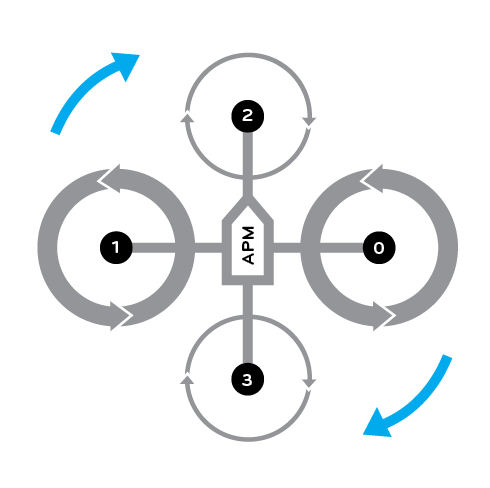
\includegraphics[width=60mm]{quadrotor-rotating}
    \caption{Giro a la derecha.} 
  \end{subfigure}
  \hspace{5pt}
  \begin{subfigure}[]{60mm}
    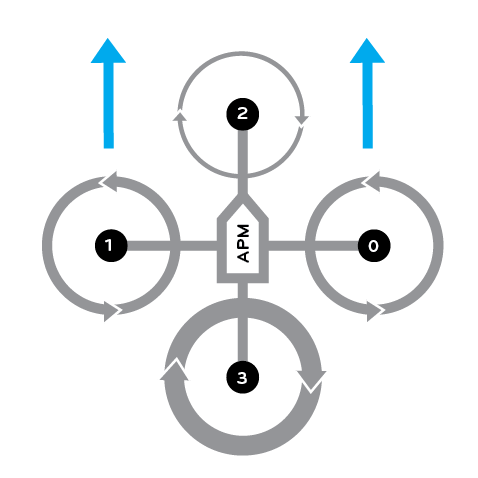
\includegraphics[width=60mm]{quadrotor-forward}
    \caption{Movimiento hacia delante.}
  \end{subfigure}
  \caption{Distintas configuraciones de los motores del cuadricóptero para desplazarse.}\label{fig:quadrotor_movements}
\end{figure}


\subsection{Aplicaciones de los drones}

Debido al auge de los cuadricópteros en los últimos tiempos se han desarrollado proyectos con ellos como elemento principal. Aquí resaltamos algunas de ellas que nos parecen interesantes y representativas.\\

\subsubsection{Lily Drone} 

Lily\footnote{https://www.lily.camera} es un cuadricóptero de reducidas dimensiones y peso (1.3kg) el cuál va equipado con una cámara capaz de grabar vídeo hasta resolución de alta definición a 1080p y 120fps. Lo más llamativo de este drone no son sus capacidades de vuelo ya que sólo nos permite vuelos de hasta 15 metros de altura y unos 40km/h de velocidad, si no que simplemente llevando un dispositivo de detección de reducidas dimensiones (28g), lo enciendes y él, sin necesidad de configuración, lo detecta y sigue todos sus movimientos mientras a la vez te está grabando. Los vuelos son de unos 20 minutos de duración, y el drone es resistente al agua, por lo que puedes usarlo prácticamente en cualquier tipo de situación. Uno de sus puntos fuertes es su funcionamiento en tres pasos, como muestra la figura \ref{fig:lily} (b).\\

\begin{figure}[htb]
\centering
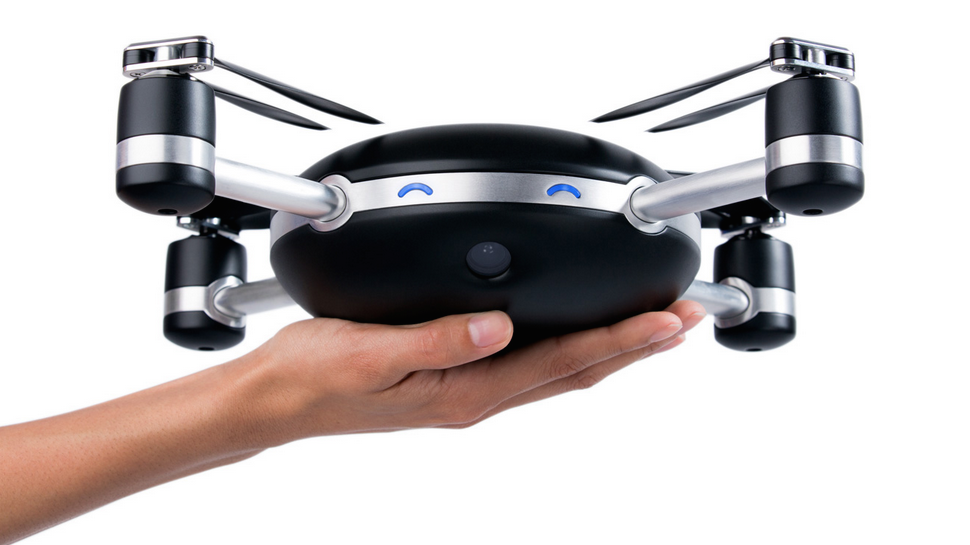
\includegraphics[width=0.7\textwidth]{lily1}
\end{figure}

\begin{figure}[htb]
\centering
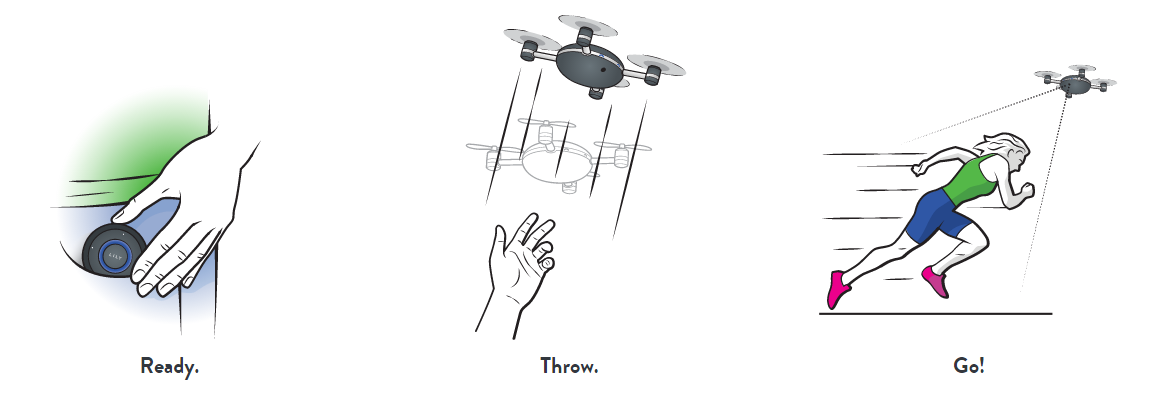
\includegraphics[width=1\textwidth]{lily2}
\caption{Lily (a) y funcionamiento en 3 pasos (b).}
\label{fig:lily}
\end{figure}

\subsubsection{Revisión del tendido eléctrico con drones}

La compañía eléctrica Endesa ha comprado una flota de catorce drones para la revisión de las líneas eléctricas en España. Los drones cuentan con cámara de alta resolución y termográfica. Con el uso de estos aparatos se agilizan las inspecciones, se mejora la calidad y ofrecen mayor seguridad al no tener que trabajar el operario sobre la red. Esto a su vez hace que no sea necesario cortar el suministro eléctrico. La figura \ref{fig:droneendesa} muestra un drone realizando servicios de revisión del tendido eléctrico.\\

\begin{figure}[h!]
\centering
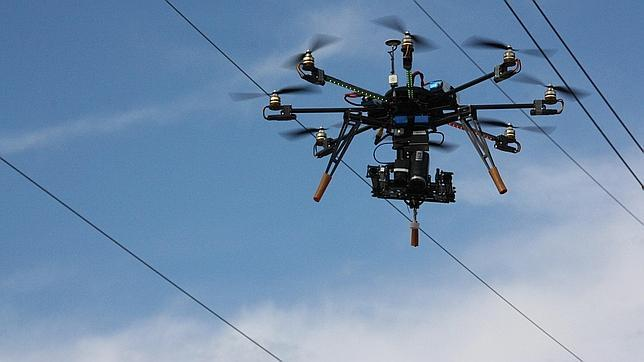
\includegraphics[width=0.8\textwidth]{dronendesa}
\caption{Drone de Endesa realizando labores de revisión.}
\label{fig:droneendesa}
\end{figure}


\subsubsection{Hemav, Agricultura de precisión.}

La empresa Hemav\footnote{http://hemav.com} ofrece entre otros servicios agricultura de precisión a través del vuelos con cuadricópteros. Utilizan sensores multiespectrales y/o térmicos para generar mapas aéreos mediante vuelos autónomos que su suministran información relevante para la toma de decisiones (\ref{fig:hemav} (b)).\\

Posteriormente esa información es analizada estadísticamente para generar patrones de estados, similitudes de terreno, detección de patologías, etc, con los que finalmente se genera un informe con las conclusiones especificas.\\

\begin{figure}[h!]
\centering
  \begin{subfigure}[]{60mm}
    \includegraphics[width=60mm]{hemav2}
    \caption{Hemav.} 
  \end{subfigure}
  \hspace{5pt}
  \begin{subfigure}[]{60mm}
    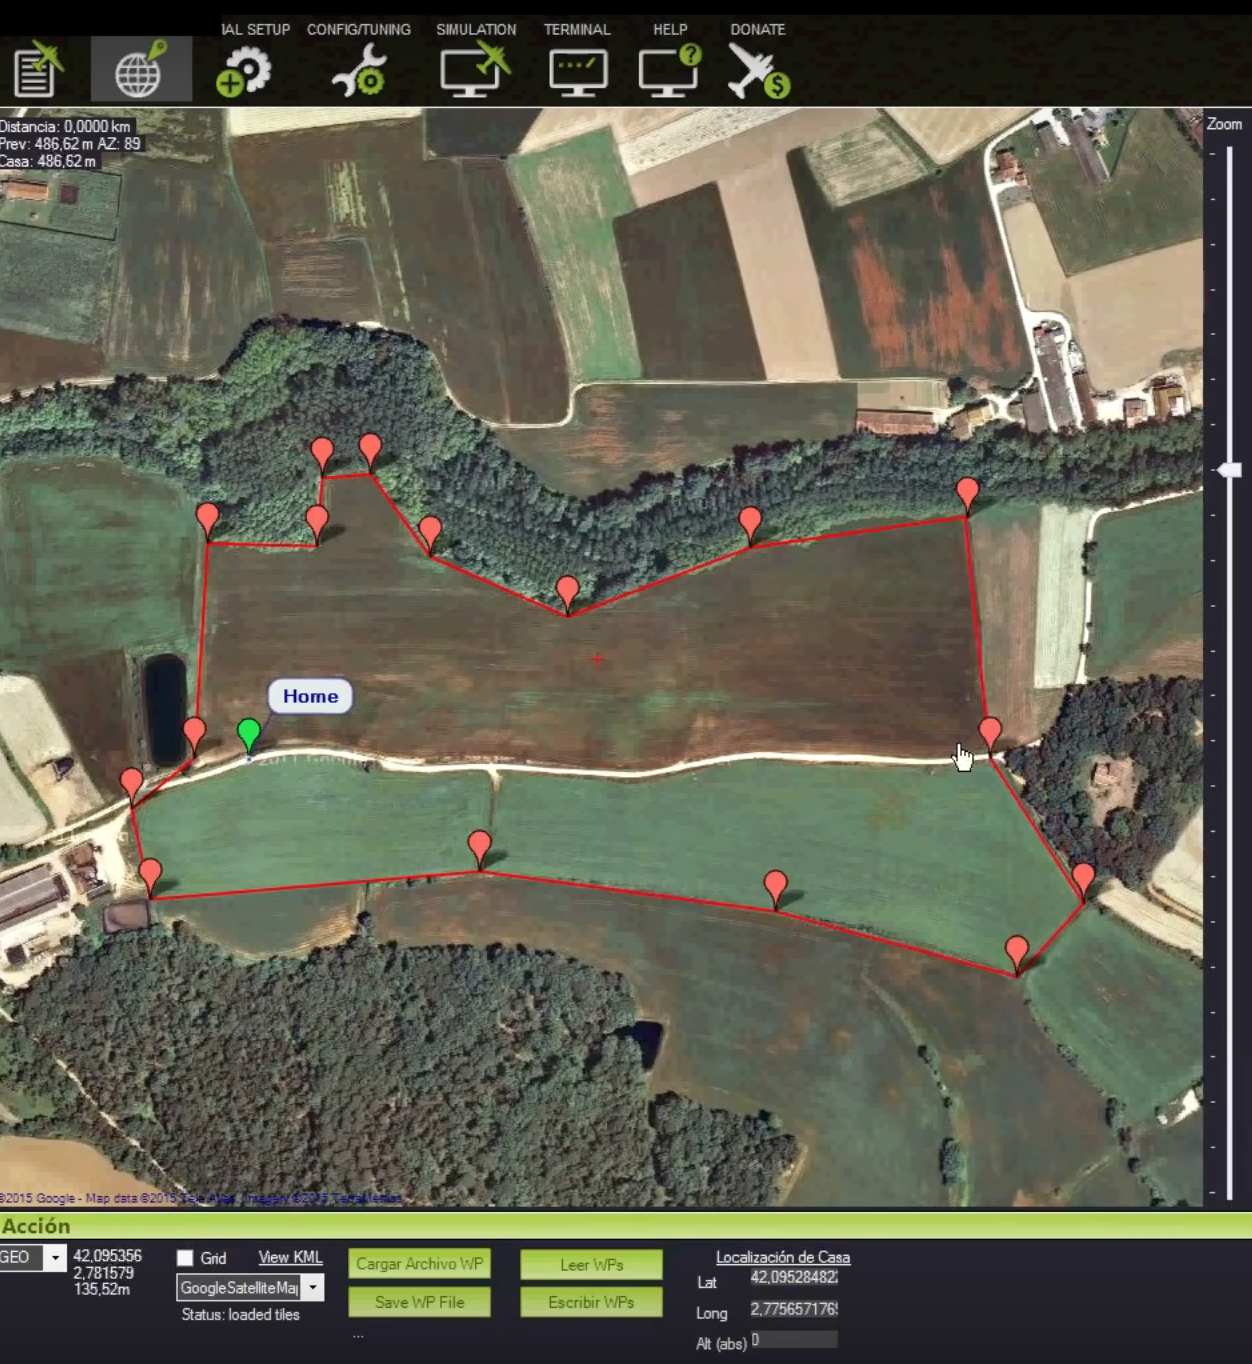
\includegraphics[width=60mm]{hemav1}
    \caption{Finca acotada para el vuelo autónomo.}
  \end{subfigure}
    \caption{Uso de drones en agricultura de precisión.}\label{fig:quadrotor_movements}
  \label{fig:hemav}
\end{figure}


\subsubsection{Entrega de paquetes con drones.}

La entrega de paquetería usando vehículos aéreos no tripulados es el futuro, aunque ya muy presente en prototipos en cuanto a la entrega de paquetes a domicilio se refiere. Las funcionalidades son numerosas, desde entrega de comida o compras realizadas a domicilio, hasta entrega de medicamentos o comida a personas en apuros o situaciones peligrosas.\\

Empresas como Amazon con su proyecto \emph{Prime Air} (figura \ref{fig:amazon}), DHL, Google con \emph{Project Wing} o la NASA están trabajando para desarrollar sus propios sistemas de entrega de paquetería a domicilio a través de drones.\\

\begin{figure}[h!]
\centering
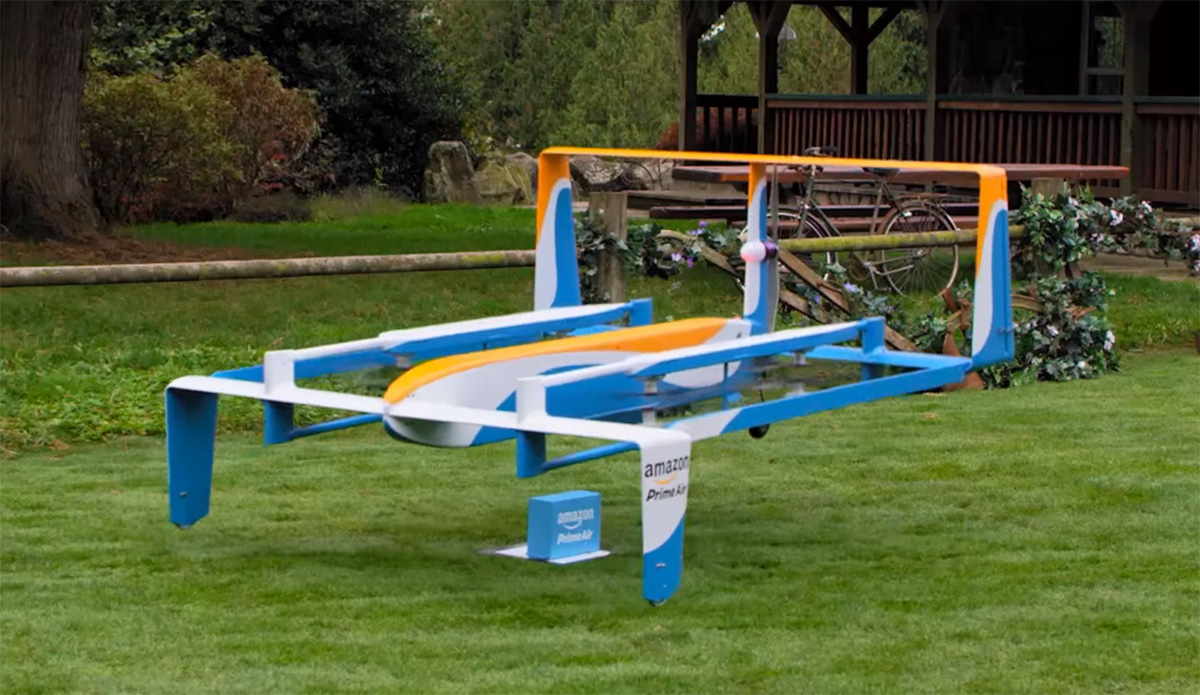
\includegraphics[width=0.9\textwidth]{amazon}
\caption{Amazon Prime Air}
\label{fig:amazon}
\end{figure}

\subsubsection{Drones en salvamento marítimo.}

La Agencia de Medios de Vodafone (MEC) y los expertos de Trabajos con Dron\footnote{trabajoscondrone.com} (TcD) han desarrollado un proyecto de drones socorristas. Estos reducen hasta en tres veces el tiempo en llegar al lugar del accidente con respecto al socorrista tradicional.\\

En caso de incidente, el socorrista-piloto conducirá el drone con el mando de radiocontrol ayudándose de la cámara que lleva a bordo, cuando llega al punto de incidencia lanzara un par de flotadores a los que se pueden agarrar hasta que llegue el equipo de salvamento.\\

En la figura figura \ref{fig:socorrista} se puede ver a un piloto de drones realizando pruebas de salvamento marítimo con un drone.||

 \begin{figure}[h!]
\centering
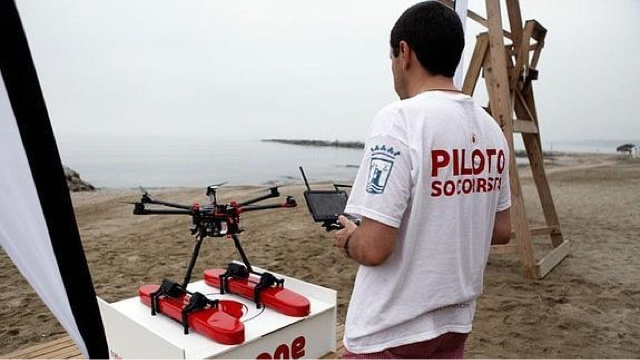
\includegraphics[width=0.9\textwidth]{socorrista}
\caption{Drone de Salvamento Marítimo}
\label{fig:socorrista}
\end{figure}

\subsubsection{Drones en el cine y televisión.}

Hace tiempo que los robots teledirigidos participan en los rodajes, pero sólo recientemente han pasado de tener un papel secundario a convertirse en protagonistas. En la industria cinematográfica se ha añadido el uso del drone para grabar escenas que antes eran complicadas, costosas o imposibles de grabar. Han cobrado tanta importancia que hasta han creado certámenes como el \emph{Flying Robot International Film Festival}\footnote{http://friff.co} para premiar su uso en la grabación. Los drones nos proporcionan nuevas perspectivas en todo tipo de secuencias.\\

Películas como el Lobo de Wall Street, Jurassic World o Skyfall han incorporado entre sus métodos de grabación la utilización de drones. También se utilizan en el mundo de la televisión. Entre otros el famoso programa inglés \emph{Top Gear} o el documental de la BBC Planeta Tierra. En la figura \ref{fig:dronefilm} podemos ver un drone grabando una escena.\\

\begin{figure}[h!]
\centering
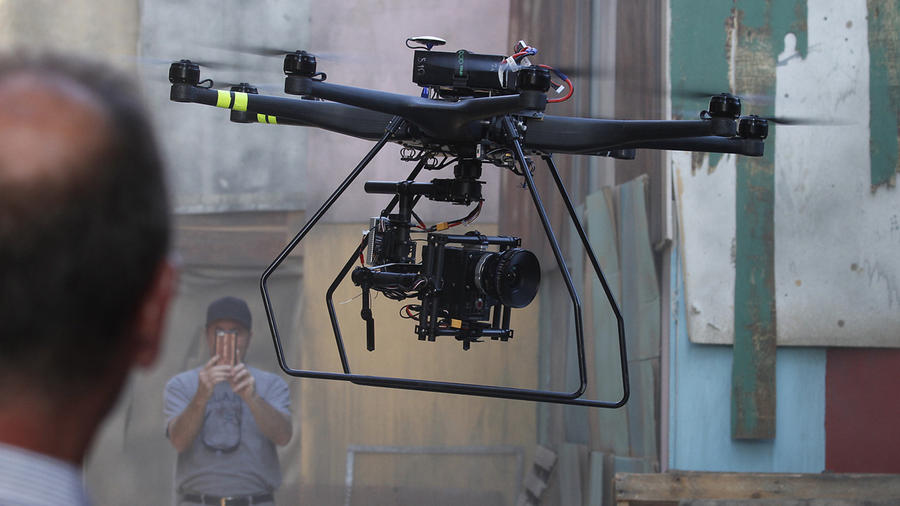
\includegraphics[width=0.9\textwidth]{dronefilm}
\caption{Uso de un drone para grabación.}
\label{fig:dronefilm}
\end{figure}



\subsection{Sistemas de control de drones}
\label{cap:controldrones}

Hay varios sistemas que nos permiten teleoperar o controlar un drone, los cuáles se pueden dividir en dos grupos, los controlados mediante radiofrecuencia y los que usan sistemas alternativos.\\

\emph{\textbf{Radiocontrol:}} Es la técnica que permite el gobierno de un objeto a distancia de manera inalámbrica mediante una emisora de control remoto. Por otra parte, a bordo del vehículo, en nuestro caso un drone, debe ir una receptora de radio control. La comunicación entre receptor y transmisor se efectúa mediante radiofrecuencia, existiendo diferentes sistemas de emisión, como AM, FM o 2.4Ghz con diferentes tipo de codificación, PCM, PPM…\\

Estos sistemas tienen varias limitaciones. Una es el número de canales máximo del sistema, ya que se usa un canal para cada elemento de control disponible: elevación, giro, rotación… La segunda, y posiblemente más crítica, son las interferencias. Si se producen interferencias ya sea por ruido o por varios emisores trabajando en las cercanías se puede perder el control de la aeronave produciendo una posible colisión, destruir la misma o incluso dañar a personas.\\
 

\emph{\textbf{Sistemas alternativos:}} A parte del radiocontrol tenemos el control a través de WiFi. Este sistema consiste en la creación de una red WiFi por parte del drone a la cual se conecta el dispositivo con el que se maneja. Este dispositivo puede ser un mando diseñado y comercializado por la propia marca o un dispositivo móvil, el cuál usa una aplicación que es la que gestiona la conexión y transferencia de datos.\\

La ventaja de estos sistemas es el ahorro de batería, ya que los transmisores y antenas WiFi necesitan de menos potencia para cubrir las mismas distancias que los sistemas tradicionales de radiocontrol. Además, el ancho de banda que nos proporciona es bastante elevado y podremos transferir tanto datos como las imágenes de las cámaras HD a bordo del drone.\\

Empresas como DJI usan sistemas mixtos que consisten en teleoperar el drone vía radiocontrol, pero la gestión y visualización de la cámara se realiza mediante una conexión WiFi como la explicada anteriormente.\\
 
La empresa francesa Parrot, la cual tiene una flota de diversos modelos de drones, utiliza un sistema de red WiFi, a la cuál conectas un dispositivo móvil ya sea Android o iOS, y mediante una aplicación desarrollada por ellos se puede teleoperar el drone, así como tener otras funcionalidades como la grabación de vídeo, captura de imágenes y gestión de parámetros de vuelo como altura o velocidad máxima. En capítulos posteriores profundizaremos en este sistema implementado, ya que es el que usaremos como referencia para desarrollar el nuestro. En la figura \ref{fig:wifiardrone} se muestra cómo se teleopera el cuadricóptero ArDrone 2.0 de Parrot.\\


\begin{figure}[h!]
\centering
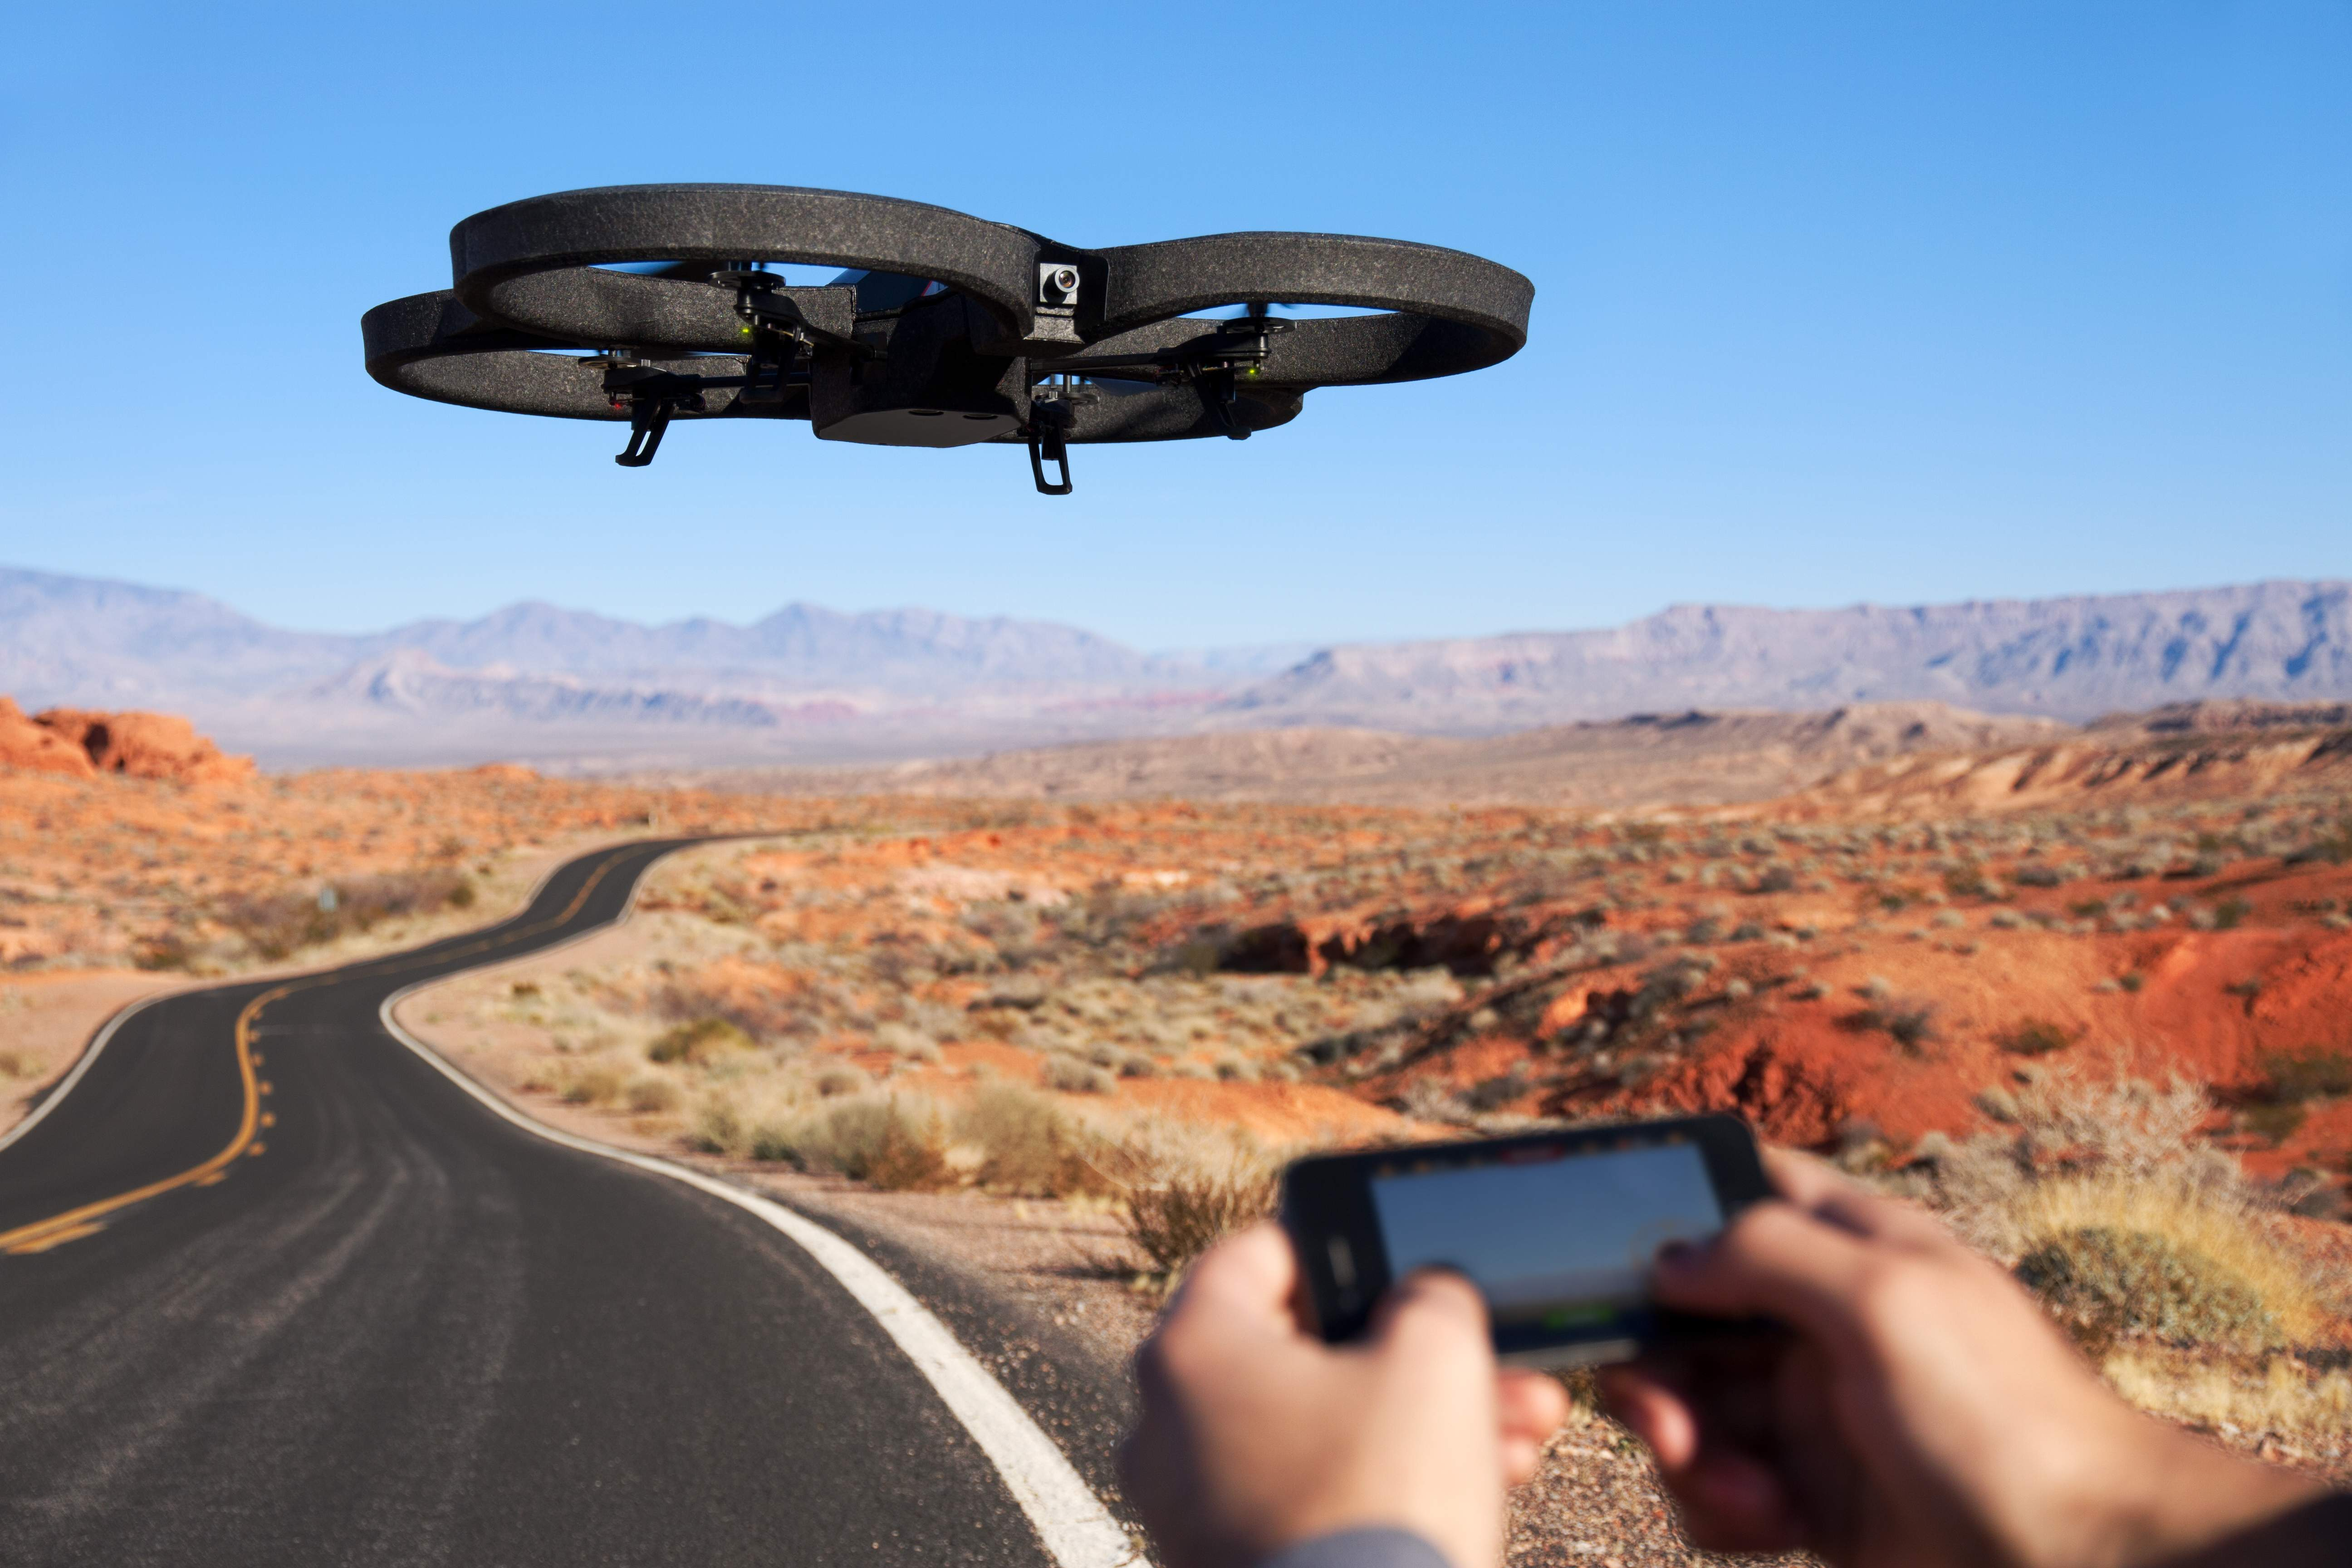
\includegraphics[width=0.8\textwidth]{wifiardrone}
\caption{Sistema WiFi de control del drone de Parrot.}
\label{fig:wifiardrone}
\end{figure}


\section{Tecnologías de comunicación en tiempo real}

En la actualidad  existen numerosas tecnologías de comunicación en tiempo real, pero nos centraremos en las que nos ofrecen conectividad multimedia. Primero veremos protocolos que se pueden implementar en aplicaciones de escritorio, y posteriormente veremos los protocolos web más actuales.\\

\subsection{RTP}

\emph{RTP} son las siglas de \emph{Real-time Transport Protocol} o Protocolo de Transporte en Tiempo Real, el cuál es un protocolo para aplicaciones de escritorio y de nivel de sesión utilizado para la transmisión de información en tiempo real, como por ejemplo audio, vídeo y datos. Está desarrollado por el grupo de trabajo de transporte de audio y vídeo del IETF (\emph{Internet Engineering Task Force}). Este protocolo es la base de la industria de Voz sobre IP (\emph{VoIP}).\\

Se encapsula sobre UDP y usa un puerto de usuario para cada medio que transfiere. Admite direcciones de destino tanto \emph{unicast} como \emph{multicast}. Se encarga de enviar cualquier tipo de trama generada por cualquier algoritmo de codificación como H261, MPEG-1, MPEG-2... pero no añade ningún tipo de fiabilidad ni de calidad del servicio (\emph{QoS}). Lo único que incorpora son marcas de tiempo para evitar el tembleque o \emph{jitter} y la sincronización entre flujos en el destino y números de secuencia para detectar pérdidas en un flujo.\\

RTP trabaja junto con otros dos protocolos que lo complementan. El primero es RTCP (\emph{Real time Control Protocol}), protocolo que proporciona información de control sobre la calidad de la transmisión. Transmite paquetes periódicos asociados a cada flujo RTP que incluye los detalles sobre los participantes, si hubiese más de uno, y las estadísticas de pérdidas que permiten el control de flujo y congestión. Según estas estadísticas se puede hacer codificación adaptativa para adaptarse al medio. También trabaja sobre UDP y usa un número de puerto superior al que usa el flujo de RTP.\\

El segundo es RTSP (\emph{Real Time Streaming Protocol}), protocolo que permite realizar un control remoto de sesión de transmisión multimedia. Es un protocolo independiente del protocolo de transporte, basado en texto que permite recuperar un determinado medio de un servidor o grabar una multiconferencia.\\

La norma define también el protoclo SRTP (\emph{Secure Real-time Transport Protocol}), el cuál es una extensión del perfil de RTP para conferencias de audio y vídeo que puede usarse para proporcionar confidencialidad, autenticación de mensajes y protección de reenvío para flujos de audio y vídeo.\\


\begin{figure}[h!]
\centering
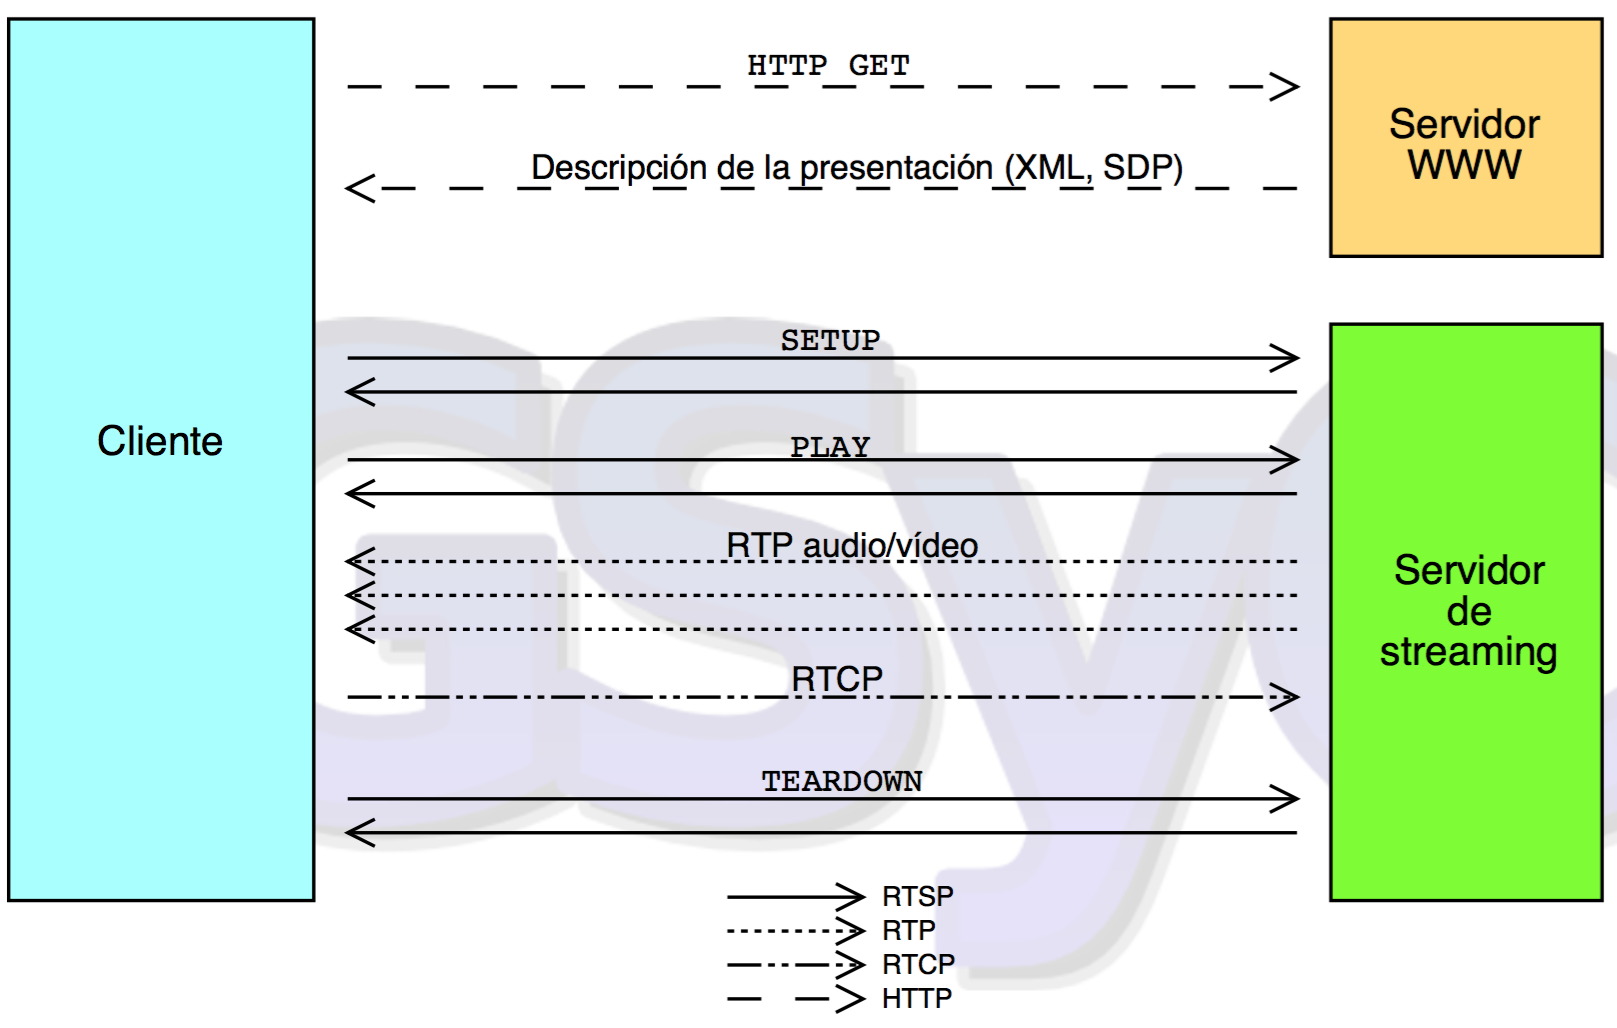
\includegraphics[width=0.8\textwidth]{rtc}
\caption{Ejemplo de conexión RTC, RTCP y RTSP}
\label{fig:rtc}
\end{figure}


\subsection{SIP}

SIP o Protocolo de Inicio de Sesiones (\emph{Session Initiation Protocol}) es un protocolo desarrollado por el grupo de trabajo MMUSIC del IETF con la intención de ser el estándar para la iniciación, modificación y finalización de sesiones interactivas de usuario donde intervienen elementos multimedia como vídeo, voz, mensajería instantánea...\\

Técnicamente no es un protocolo que transmite flujos multimedia, si no que es un protocolo de señalización cuya función es preparar el establecimiento y la terminación de sesiones multimedia entre máquinas remotas. Una de sus más importantes funciones es el intercambio de las descripciones de sesión (\emph{SDP}) de los usuarios. El concepto de sesión en este protocolo es muy amplio: una llamada entre dos, una videoconferencia, un juego interactivo entre varios usuarios...\\

Es un protocolo muy ligero. Tiene solo 6 métodos basados en texto, de manera similar a HTTP o SMTP, pero es completamente independiente del protocolo de transporte utilizado (TCP, UDP, ATM, etc). \\

En la figura \ref{fig:sip} podemos ver un ejemplo de una conexión multimedia con RTP que utiliza el protocolo SIP para establecer y finalizar la sesión entre los dos usuarios.\\

Es el protocolo señalizador para el protocolo RTP explicado anteriormente. Entre otras, Ekiga, WengoPhone, MS Windows Messenger, Apple iChat AV ó Asterisk son algunas aplicaciones que utilizan SIP.\\


\begin{figure}[h!]
\centering
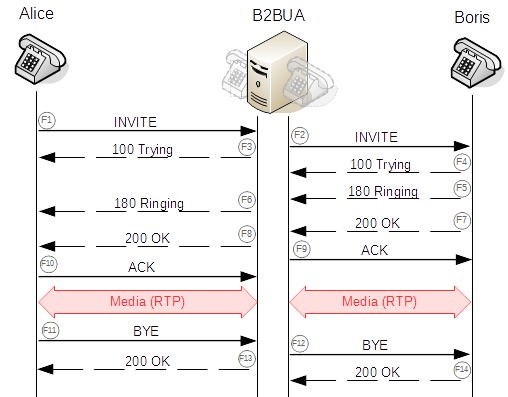
\includegraphics[width=0.8\textwidth]{sip}
\caption{Ejemplo de conexión SIP}
\label{fig:sip}
\end{figure}



\subsection{ORTC}

\emph{Object RTC} es un proyecto de código abierto que permite la comunicación en tiempo real (\emph{RTC, Real-Time Communications}) de dispositivos móviles con servidores u otros navegadores con el simple uso de unas API's JavaScript nativas en el navegador. El objetivo de Object RTC es permitir crear comunicaciones en tiempo real con una alta calidad en dispositivos móviles y servidores con el simple uso de JavaScript y HTML5. Es también una obligación para ORTC ser compatible con WebRTC.\\

Aunque ORTC es un proyecto respaldado por empresas de la talla de Hookflash, Microsoft o Google, por el momento no es una especificación del consorcio W3C (\emph{World Wide Web Consortium}).\\

ORTC comparte muchas similitudes con WebRTC. Como mayor diferencia tenemos que ORTC no utiliza SDP ni el protocolo de Oferta/Respuesta, en cambio utiliza los objetos 'enviador' (\emph{sender}), 'recibidor' (\emph{receiver}) y 'transporte' (\emph{transport}), los cuales tienen capacidades que describen que pueden hacer y sus parámetros que definen como están configurados. Además ORTC no está disponible nada más que en el navegador Edge de Microsoft.\\


\subsection{WebRTC}

En mayo de 2011 Google liberó un proyecto de código abierto basado en la comunicación entre navegadores en tiempo real. El proyecto ha sido continuado estandarizando los protocolos en el IETF y las API's de JavaScript en el W3C. En el consorcio W3C WebRTC es aún un borrador de un proyecto en marcha el cuál está altamente implementado en los navegadores como Mozilla Firefox y Google Chrome. La API está basada en el trabajo previo realizado por \emph{Web Hypertext Application Technology Working Group} (WHATWG).\\

Esta tecnología nos brinda la capacidad de crear numerosas aplicaciones de comunicaciones entre navegadores, sin necesidad de servidores internos, y está llamada a ser el futuro de las comunicaciones en tiempo real.\\


\section{Antecedentes}

Como base para el proyecto tenemos los siguientes trabajos, desarrollados también por alumnos de la URJC. Todos estos proyectos tienen en común que utilizan como base las herramientas que nos ofrece JdeRobot, que es el marco \emph{software} en el que se ubica el presente trabajo.\\

\subsection{ArDroneServer}

ArDroneServer\footnote{\url{http://jderobot.org/Amartinflorido-tfg}}\cite{ArDroneServer} es un \emph{driver} para manejar drones desde la plataforma JdeRobot. Utiliza la SDK de ArDrone de Parrot, ha sido desarrollado por Alberto Martín como parte de su Grado Fin de Carrera. Esta aplicación esta inspirada en los paquetes ROS \emph{ardrone\_brown} y \emph{ardrone\_autonomy}. Implementa tres interfaces que nos permites recibir las imágenes del drone, controlar el drone y recoger información de los sensores y cambiar la configuración del drone. Junto a este servidor Alberto ha desarrollado una aplicación capaz de hacer seguimiento horizontal y vertical de objetos.\\

En la figura \ref{fig:ardroneserveralberto} vemos a Alberto realizando un experimento, en el que el drone hace seguimiento vertical de un objeto.\\

\begin{figure}[h!]
\centering
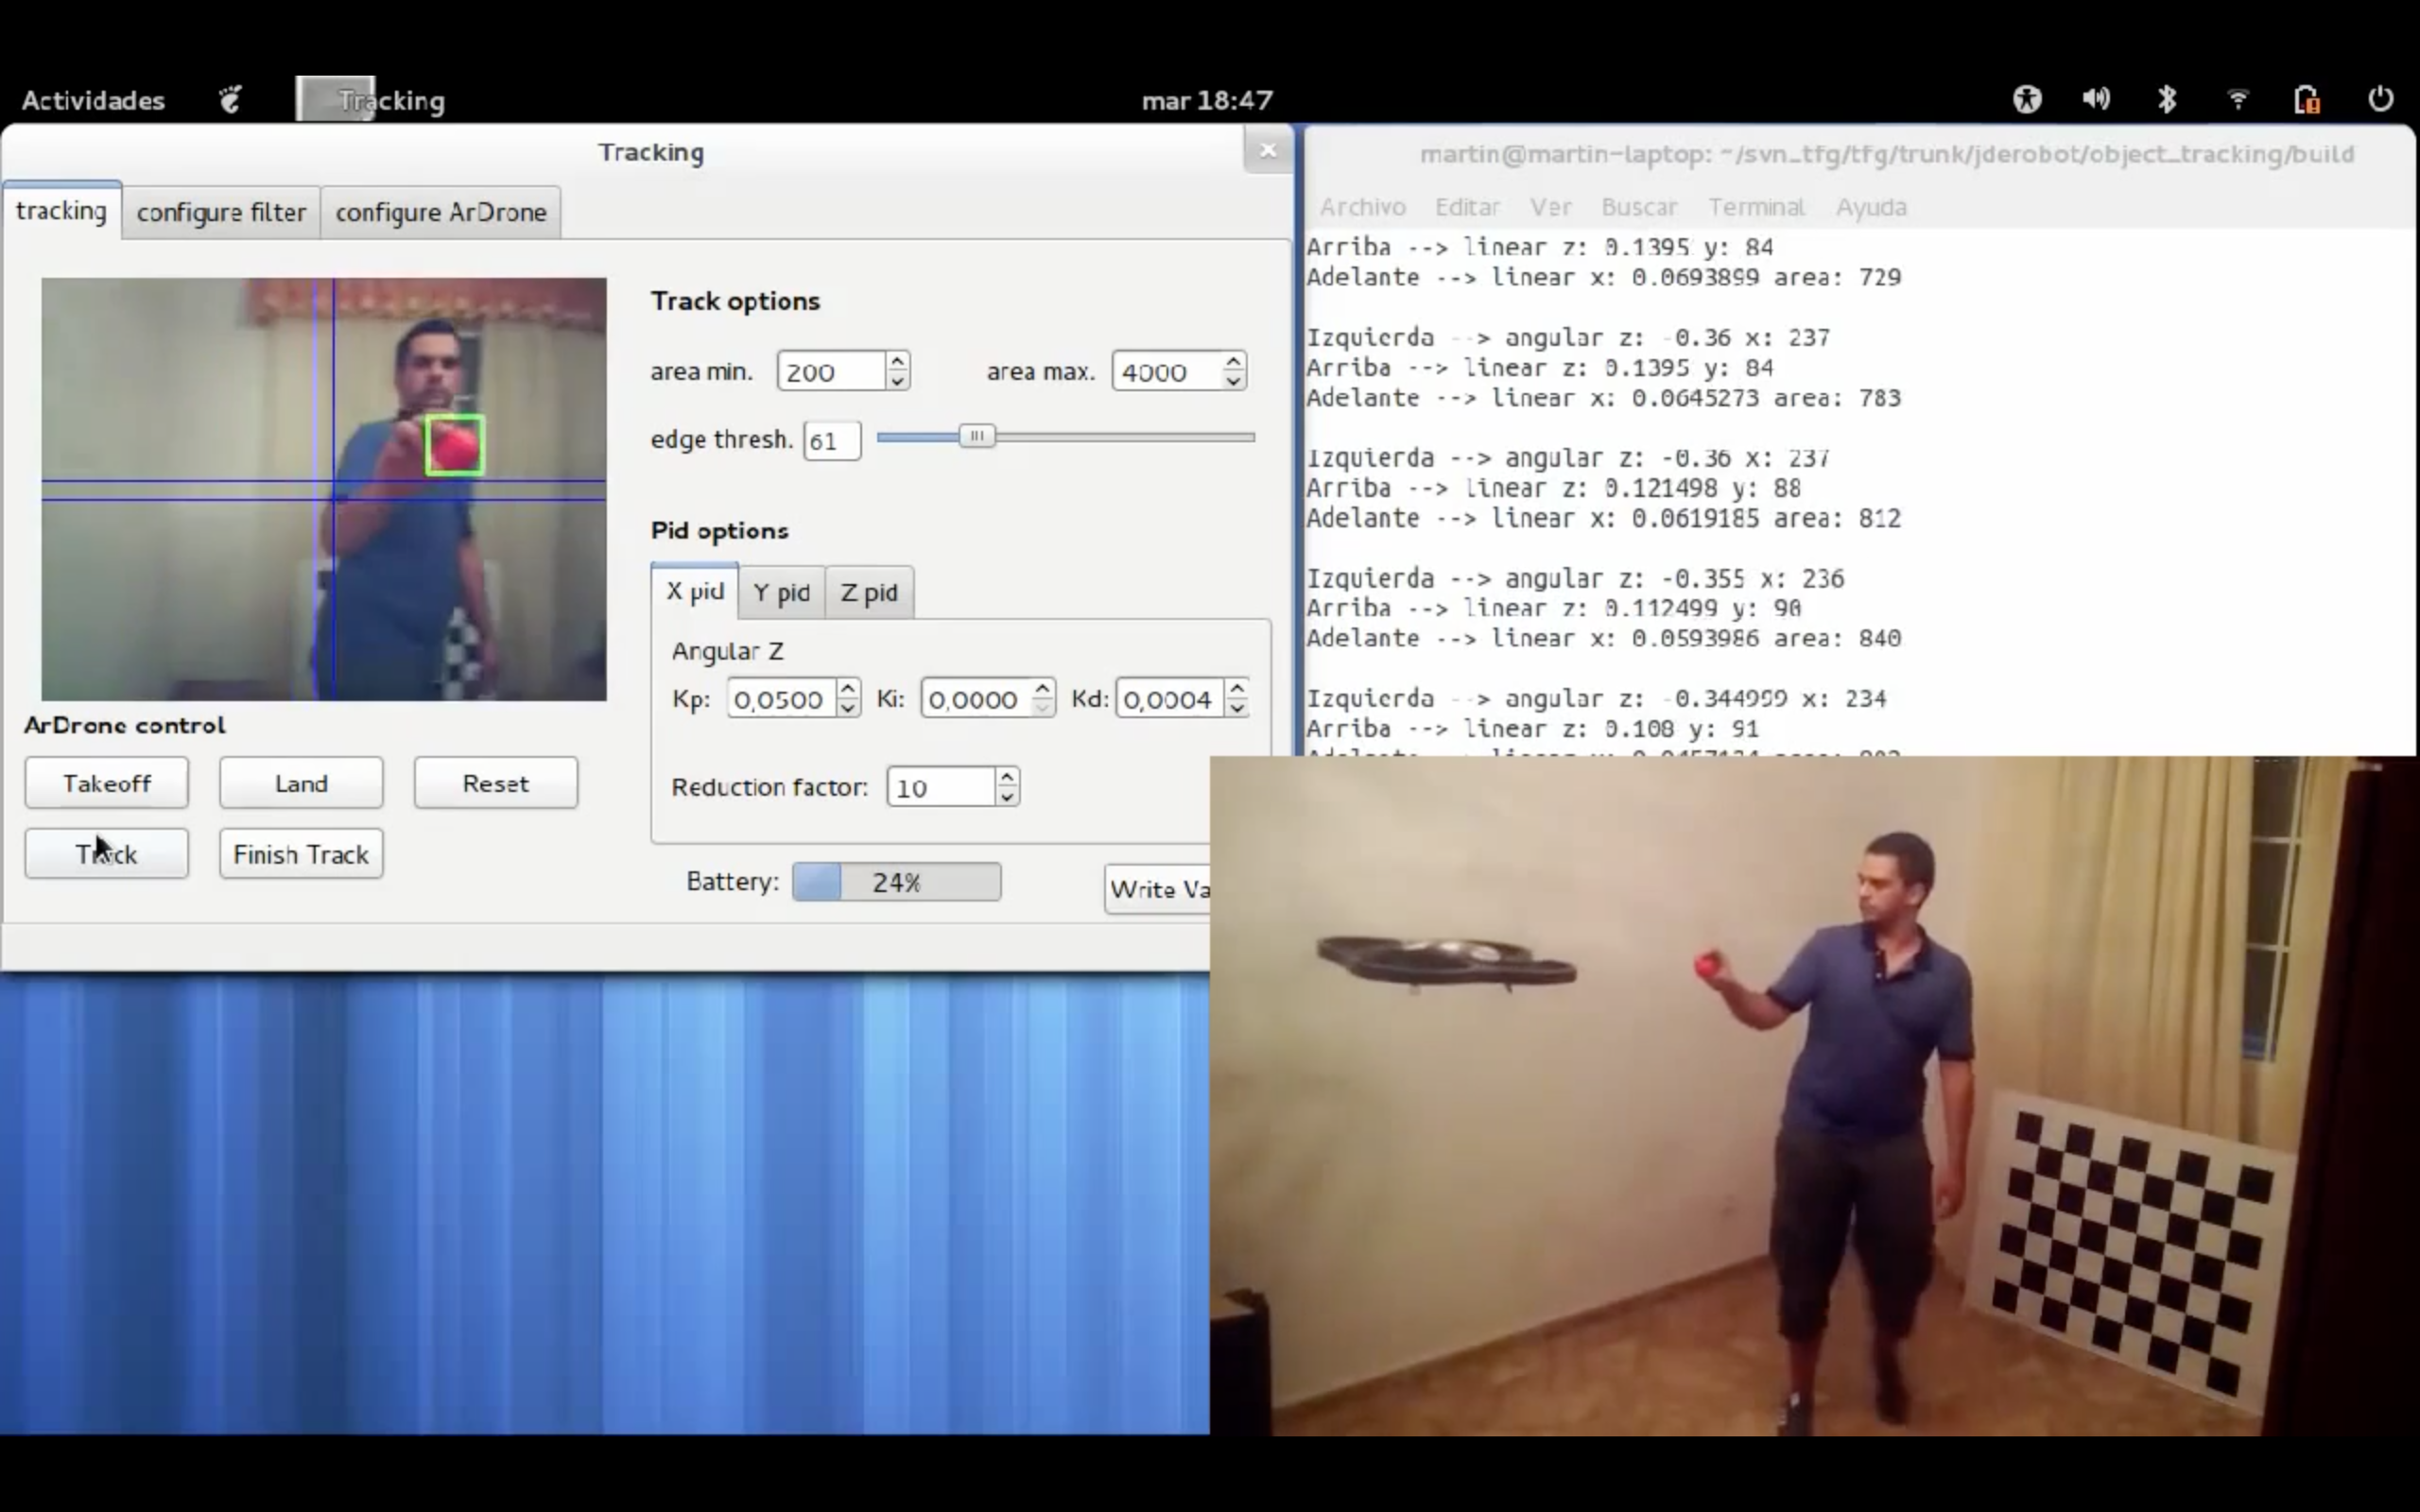
\includegraphics[width=0.9\textwidth]{ardroneserver_alberto}
\caption{Seguimiento horizontal usando ardrone\_server.}
\label{fig:ardroneserveralberto}
\end{figure}

\subsection{Surveillance 4.0}

Surveillance 4.0\footnote{\url{http://jderobot.org/D. castellanob-pfc}}\cite{surveillance4.0} es un ejemplo de conexión web con sensores y actuadores, desarrollado por Daniel Castellano como su Proyecto Fin de Carrera. Esta aplicación contaba con varios sensores de distinto tipo (humedad, temperatura, gas, etc) que se conectaban inalámbricamente con un nodo central situado en una Raspberry Pi. La conexión inalámbrica se hacía mediante transmisores Zigbee con un protocolo propio llamado WHAP. El nodo central recibía los datos de los sensores y los mostraba mediante un servidor web que corría en la misma máquina. La aplicación web se desarrolló en Python usando el entorno de desarrollo web Django. En Surveillance 4.0, los valores de los sensores se guardaban en una base de datos que la aplicación web consultaba cuando era necesario. Además, esta versión incluía un streaming de vídeo utilizando el software de código abierto M-JPEG Streamer. En la figura \ref{fig:surveillance4} se puede ver la aplicación.\\


\subsection{Surveillance 5.1}

Otro ejemplo de conexión web con sensores y actuadores es Surveillance 5.1\footnote{\url{http://jderobot.org/Aerobeat-colab}}\cite{surveillance5.1} desarrollado por Edgar Barrero como su Trabajo Fin de Grado. Esta aplicación obtenía un flujo de imágenes de una cámara web, un flujo de imágenes de profundidad de un sensor Kinect, además de datos de un sensor de humedad y de interaccionar con un actuador. La aplicación web se desarrolló en Ruby sobre Rails. En Surveillance 5.1, el servidor web se conectaba a los componente de JdeRobot mediante sus interfaces ICE. La aplicación web refrescaba estos datos mediante peticiones AJAX.  En la figura \ref{fig:surveillance5} se puede ver la aplicación.\\


\begin{figure}[h!]
\centering
  \begin{subfigure}[]{110mm}
    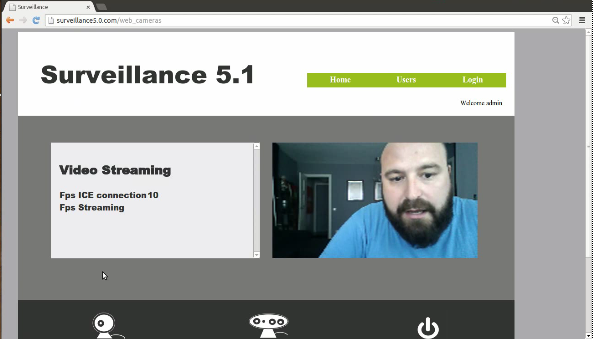
\includegraphics[width=110mm]{surveillance5}
  \end{subfigure}
  \hspace{5pt}
  \begin{subfigure}[]{110mm}
    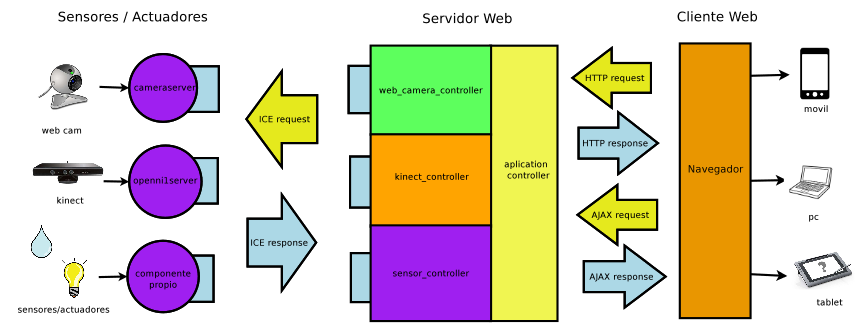
\includegraphics[width=110mm]{esquema_s5}
  \end{subfigure}
  \caption{interfaz (a) y arquitectura (b).}\label{fig:surveillance5}
\end{figure}


\subsection{Teleoperadores y visores Web en JdeRobot}

Un ejemplo ya sin servidores web intermedios, directo entre sensores, robots y navegadores web es esta plataforma desarrollada por Aitor Martínez como su Trabajo Fin de Grado\footnote{\url{http://jderobot.org/Aitormf-tfg}}\cite{teleoperadoresyvisoresweb}. Está compuesta por cuatro clientes Web: CameraViewJS, RGBDViewerJS, KobukiViewerJS y UavViewerJS, los cuales son las versiones web de las herramientas homónimas desarrolladas por JdeRobot. Estas nuevas herramientas hablan directamente con los servidores desarrollados por JdeRobot para acceder a los sensores y robots, y como diferencia principal destacable no necesitan de servidores intermedios para funcionar, utilizando \emph{websockets} para establecer las conexiones necesarias.\\

\noindent Las funcionalidades de estos clientes web son: 

\begin{enumerate}

\item \emph{CameraViewJS:} Cliente web similar a la herramienta \texttt{CameraView} para visualizar imágenes procedentes del servidor \texttt{Cameraserver}. 

\item \emph{RGBDViewerJS:} Cliente web similar a la herramienta RGBDViewer para visualizar datos de color y profundidad procedentes del servidor \texttt{Openni1Server}.
  
\item \emph{KobukiViewerJS:} Teleoperador para manejar y ver los datos de los sensores de los robots Kobuki y Pioneer del laboratorio de robótica de la URJC. Versión web de \texttt{KobukiViewer}
  
  
\item \emph{UavViewerJS:} Cliente web similar a la herramienta UavViewer para teleoperar drones tanto reales como simulados y ver los datos de sus sensores.


\end{enumerate}

\begin{figure}[h!]
\centering
\includegraphics[width=0.9\textwidth]{uavviewerjs_aitor}
\caption{Cliente web UavViewer.js}
\label{fig:introrobuavjs}
\end{figure}


En el proyecto que aquí se presenta se desarrolla una aplicación web capaz de teleoperar un cuadricóptero usando los servidores desarrollados por JdeRobot para conectarnos al drone, sus sensores y actuadores, y añadiendo la tecnología web de última generación \emph{WebRTC} para establecer la conexión entre el ordenador que se comunicará con el drone y el ordenador remoto. Desde el navegador se podrán ver los valores de los sensores y la cámara a bordo del drone, además como ya he mencionado, de teleoperarlo. Estas conexiones se realizarán sin el uso de servidor intermedio, usando tecnologías en tiempo real que se conectarán mediante \emph{WebSockets} de \emph{JavaScript}.\\


Una vez presentada la introducción y el contexto del proyecto en este capítulo, continuamos exponiendo los objetivos que nos hemos marcado. En el capítulo tres se habla sobre las infraestructuras software en las que nos hemos ayudado para el desarrollo. Posteriormente en el capítulo cuatro veremos cómo hemos conseguido cumplir los objetivos marcados, exponiendo en el capítulo cinco las pruebas y experimentos realizados. En el último capitulo presentaremos las conclusiones del proyecto.\\

\chapter{Objetivos}

Una vez situado el Trabajo Fin de Grado en su contexto vamos a presentar los objetivos concretos que nos marcamos para la realización del mismo.


\section{Objetivos}

Como objetivo global nos proponemos teleoperar un drone desde dispositivos móviles cómo teléfonos o tabletas utilizando tecnologías web de ultima generación. Este objetivo se ha desglosado en tres subobjetivos concretos que explicamos a continuación.\\

Como escenario nos encontramos con un ordenador que irá a bordo del drone, y un navegador en una máquina remota. Durante toda la memoria nos referiremos como ordenador local, par local o navegador local al dispositivo que usaremos para conectarnos al cuadricóptero y el cuál deberá ir a bordo del drone, y ordenador remoto, par remoto o navegador remoto al ordenador desde el cuál teleoperaremos el vehículo.\\

\begin{itemize}


\item \emph{\textbf{Conexión local}}: Como primer subobjetivo tenemos que desarrollar una conexión directa del navegador local con el \emph{hardware} del drone. Esta conexión tiene que ser bidireccional, ya que tenemos que acceder a los sensores y actuadores del drone, así como a su cámara, pero también es necesario mandarle órdenes de movimiento.\\

Como requisito fundamental para esta conexión con el servidor de los actuadores y sensores a bordo es que tiene que ser en tiempo real y que sea lo suficientemente fluida y ligera como para que no introduzca ningún tipo de retardo.\\


\item \emph{\textbf{Conexión multimedia entre navegadores}}: El segundo punto con el que nos enfrentamos es utilizar una tecnología web moderna y actual con la que poder teleoperar el drone. Esta tecnología tiene que ser lo suficientemente versátil como para poder implementarla en nuestro proyecto. Por otro lado, al igual que la conexión local, tiene que ser bidireccional, poder transportar audio, vídeo y datos genéricos e introducir el mínimo retraso en la comunicación posible para tener una experiencia positiva y controlada del vuelo del drone.\\

Esta conexión deberá realizarse entre el ordenador local y un segundo ordenador, que será desde el que el usuario podrá teleoperar el vehículo.\\


\item \emph{\textbf{Interfaz de usuario amigable}}: Uno de los subobjetivos es desarrollar una interfaz web de usuario clara, que nos muestre de una manera lo más realista, clara y concisa posible los datos recogidos de los sensores del drone y la cámara para permitirnos conocer el estado de vuelo del drone en cada momento: altitud, inclinación, velocidad...\\

Esta interfaz deberá permitirnos el manejo del cuadricóptero de la forma mas realista y similar posible a los sistemas de control de drones que hemos hablado en la sección \ref{cap:controldrones}. Para que la experiencia de vuelo sea satisfactoria la interfaz tiene que tener unos controles de movimiento que sean sencillos, simples e intuitivos.\\

\end{itemize}


\section{Metodología y plan de trabajo}

La realización de un proyecto requiere una metodología que establezca las pautas a seguir y la planificación de las tareas que se deben llevar a cabo para cumplir los objetivos. Hemos escogido el modelo de \emph{desarrollo en espiral}, ya que es un modelo ampliamente usado en la ingeniería de \emph{software}. Este modelo define una serie de ciclos que se repiten en un bucle hasta el final del proyecto, dividiéndolo en varias subtareas más sencillas y estableciendo puntos de control al final de cada iteración en los que se evalúa el trabajo realizado y se enfocan las nuevas tareas para continuar.\\

Esta metodología recibe su nombre por la forma de espiral que tiene su representación gráfica o diagrama de flujo, que podemos ver en la figura \ref{fig:planificacion_espiral}. En cada iteración se llevan a cabo las siguientes actividades:

\begin{itemize}
 \item \textbf{Determinar los objetivos}, dividir en subobjetivos y fijar requisitos.
 \item \textbf{Analizar los riesgos} y factores que impidan o dificulten el trabajo y las consecuencias negativas que este
 pueda ocasionar.
 \item \textbf{Desarrollar} las tareas para lograr los objetivos según los requisitos especificados.
 \item \textbf{Planificar} las próximas fases tras evaluar el transcurso del proyecto.
\end{itemize}

\begin{figure}[h!]
\centering
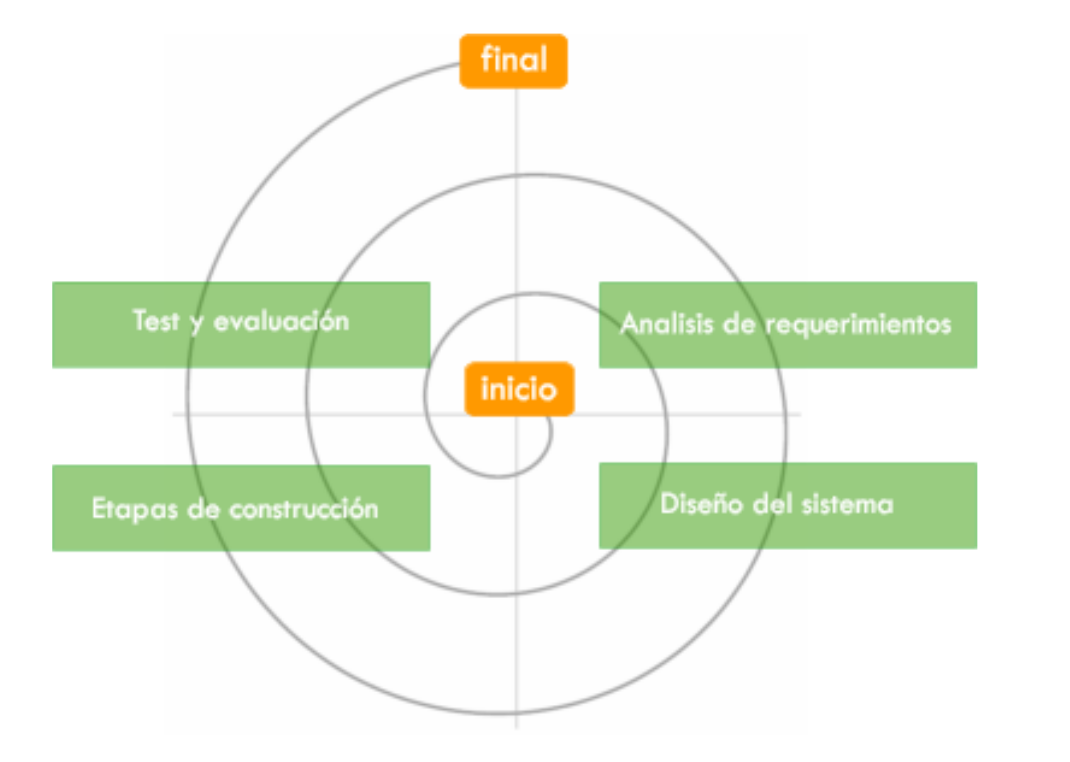
\includegraphics[width=0.9\textwidth]{espiral}
\caption{Esquema general del desarrollo del proyecto.}
\label{fig:planificacion_espiral}
\end{figure}

Durante el ciclo de vida del proyecto se han hecho reuniones periódicas con el tutor. En ellas se evaluaban los avances logrados y se marcaba la hoja de ruta a tomar para los siguientes días de desarrollo. Si los puntos marcados en sesiones anteriores no se habían finalizado se ampliaba el plazo o se intentaba buscar otra manera de avance.\\

Para facilitar el seguimiento del proyecto se ha utilizado de un mediawiki\footnote{http://jderobot.org/Irodmar-tfg} de JdeRobot en el que se iba actualizando cada avance que se lograba, con explicaciones y vídeos e imágenes. Para el código fuente se ha empleado un repositorio en la plataforma web de control de versiones GitHub\footnote{https://github.com/RoboticsURJC-students/2015-tfg-irodmar}.\\

El plan de trabajo para todo el proyecto se puede dividir en las siguientes etapas:

\begin{itemize}
\item \textbf{Familiarización con JdeRobot}: Primer contacto con esta plataforma y sus herramientas para conocer su funcionamiento.
\item \textbf{Aprendizaje de tecnologías web necesarias:} Conocer las tecnologías web que van a ser necesarias para el desarrollo del proyecto. Entre ellas se encuentra WebRTC, HTML5, CSS3, WebGL, ThreeJS, o jQuery. Primer contacto también con el \emph{middleware} ICE.
\item \textbf{Desarrollo de la conexión local:} Creación de toda la infraestructura necesaria para la interconexión entre el navegador local y el drone.
\item \textbf{Desarrollo conexión entre navegadores}: Desarrollo de la conexión remota que interconectará los dos pares.
\item \textbf{Desarrollo interfaz web de usuario}: Desarrollo de la interfaz amigable para teleoperar el drone.
\item \textbf{Experimentos}: Primero se realizan pruebas con el simulador, y cuando el código este suficientemente maduro se prueba con un drone real.
\end{itemize}







\chapter{Infraestructura Software} 

Una vez presentados los objetivos que tenemos marcados hay que echar una mirada a las tecnologías software y hardware que hemos utilizado como base en el proyecto. La más importante y sobre la que está centrado el proyecto es WebRTC. Además hemos emleado, como apoyo para cubrir las partes que WebRTC no llega, ICEJS junto con la plataforma robótica JdeRobot. Estas tecnologías junto con el simulador robótico Gazebo nos ha permitido probar, depurar y mejorar el código antes de realizar los experimentos sobre el drone real ArDrone, el cuál presento a continuación.


\section{ArDrone de Parrot}

El Parrot ARDrone es un drone que comercializa la marca Parrot el cuál puede ser teleoperado con una aplicación desde el dispositivos móviles. El drone crea una red WiFi, a la cuál conectas tu teléfono o tablet iOS ó Android y desde la aplicación, suministrada también por ña marca Parrot,  se tiene una comunicación directa con el drone.\\

A parte de esto Parrot tiene una SDK para desarrolladores la cuál es libre y está muy bien documentada para que quien quiera pueda desarrolar sus aplicaciones. Esta SDK es sobre la que JdeRobot ofrece, junto con el middleware ICE (\emph{Internet Communication Engine}), una pasarela que nos da conectividad entre el drone real y la aplicación/componente que estemos desarrollando o usando.

\begin{figure}[h!]
\centering
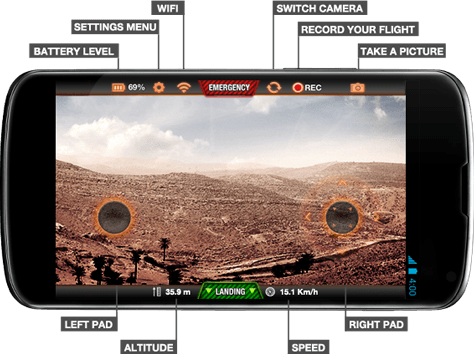
\includegraphics[width=0.6\textwidth]{ardrone_movil}
\end{figure}

\begin{figure}[h!]
\centering
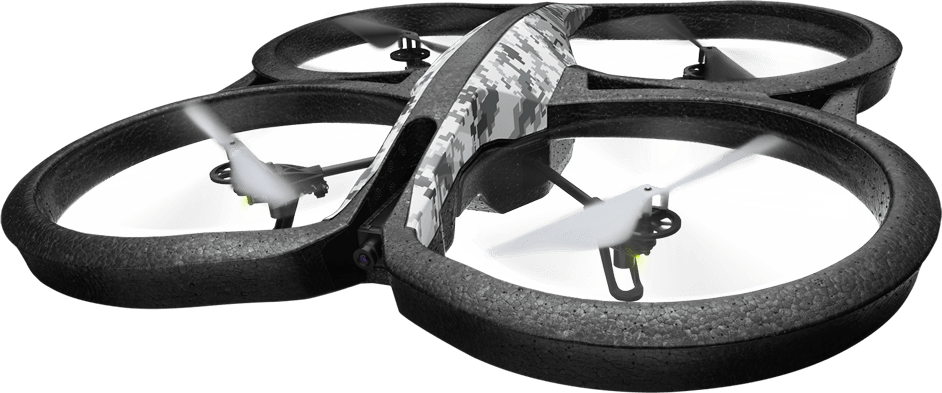
\includegraphics[width=0.6\textwidth]{ardrone}
\caption{ArDrone de Parrot}
\label{fig:ardrone}
\end{figure}

Para simular este drone de la manera mas realista y realizar las pruebas de manera virtual, nos vamos a apoyar en el simulador robótico Gazebo.


\newpage
\section{Simulador robótico Gazebo}

Gazebo es un simulador 3D de robótica desarrollado por la \textit{Open Source Robotics Foundation (OSRF)}. Es multiplataforma y entre otras cosas nos permite diseñar y crear nuestro propio robot y escenarios realistas, con obstáculos y objetos, para probar nuestros algoritmos de una forma muy parecida a las condiciones que nos vamos a encontrar en el mundo real, pero sin poner en peligro ni nuestros robots ni a ninguna persona cercana en caso de que se comporte de una forma inesperada. Para conseguir este realismo y potencia Gazebo cuenta con un motor físico para la mecánica, iluminación, gravedad, inercia... Uno de los puntos más favorables de este simulador es que es libre y tiene una comunidad muy numerosa y participativa.\\

JdeRobot tiene desarrollado el componente para Gazebo que contiene el modelo, el mundo y los plugin necesarios para simular el ArDrone de Parrot, de tal manera que podremos testear el código para ir puliendo y conseguir que sea lo suficientemente estable para posteriormente poder probarlo en el drone real.\\

Se ha usado la versión 5.1 del simulador, la cuál es última version estable a la fecha de comienzo y 100% compatible con el plugin de JdeRobot mencionado, el cuál se explica a continuación más en profundidad.\\

\begin{figure}[h!]
\centering
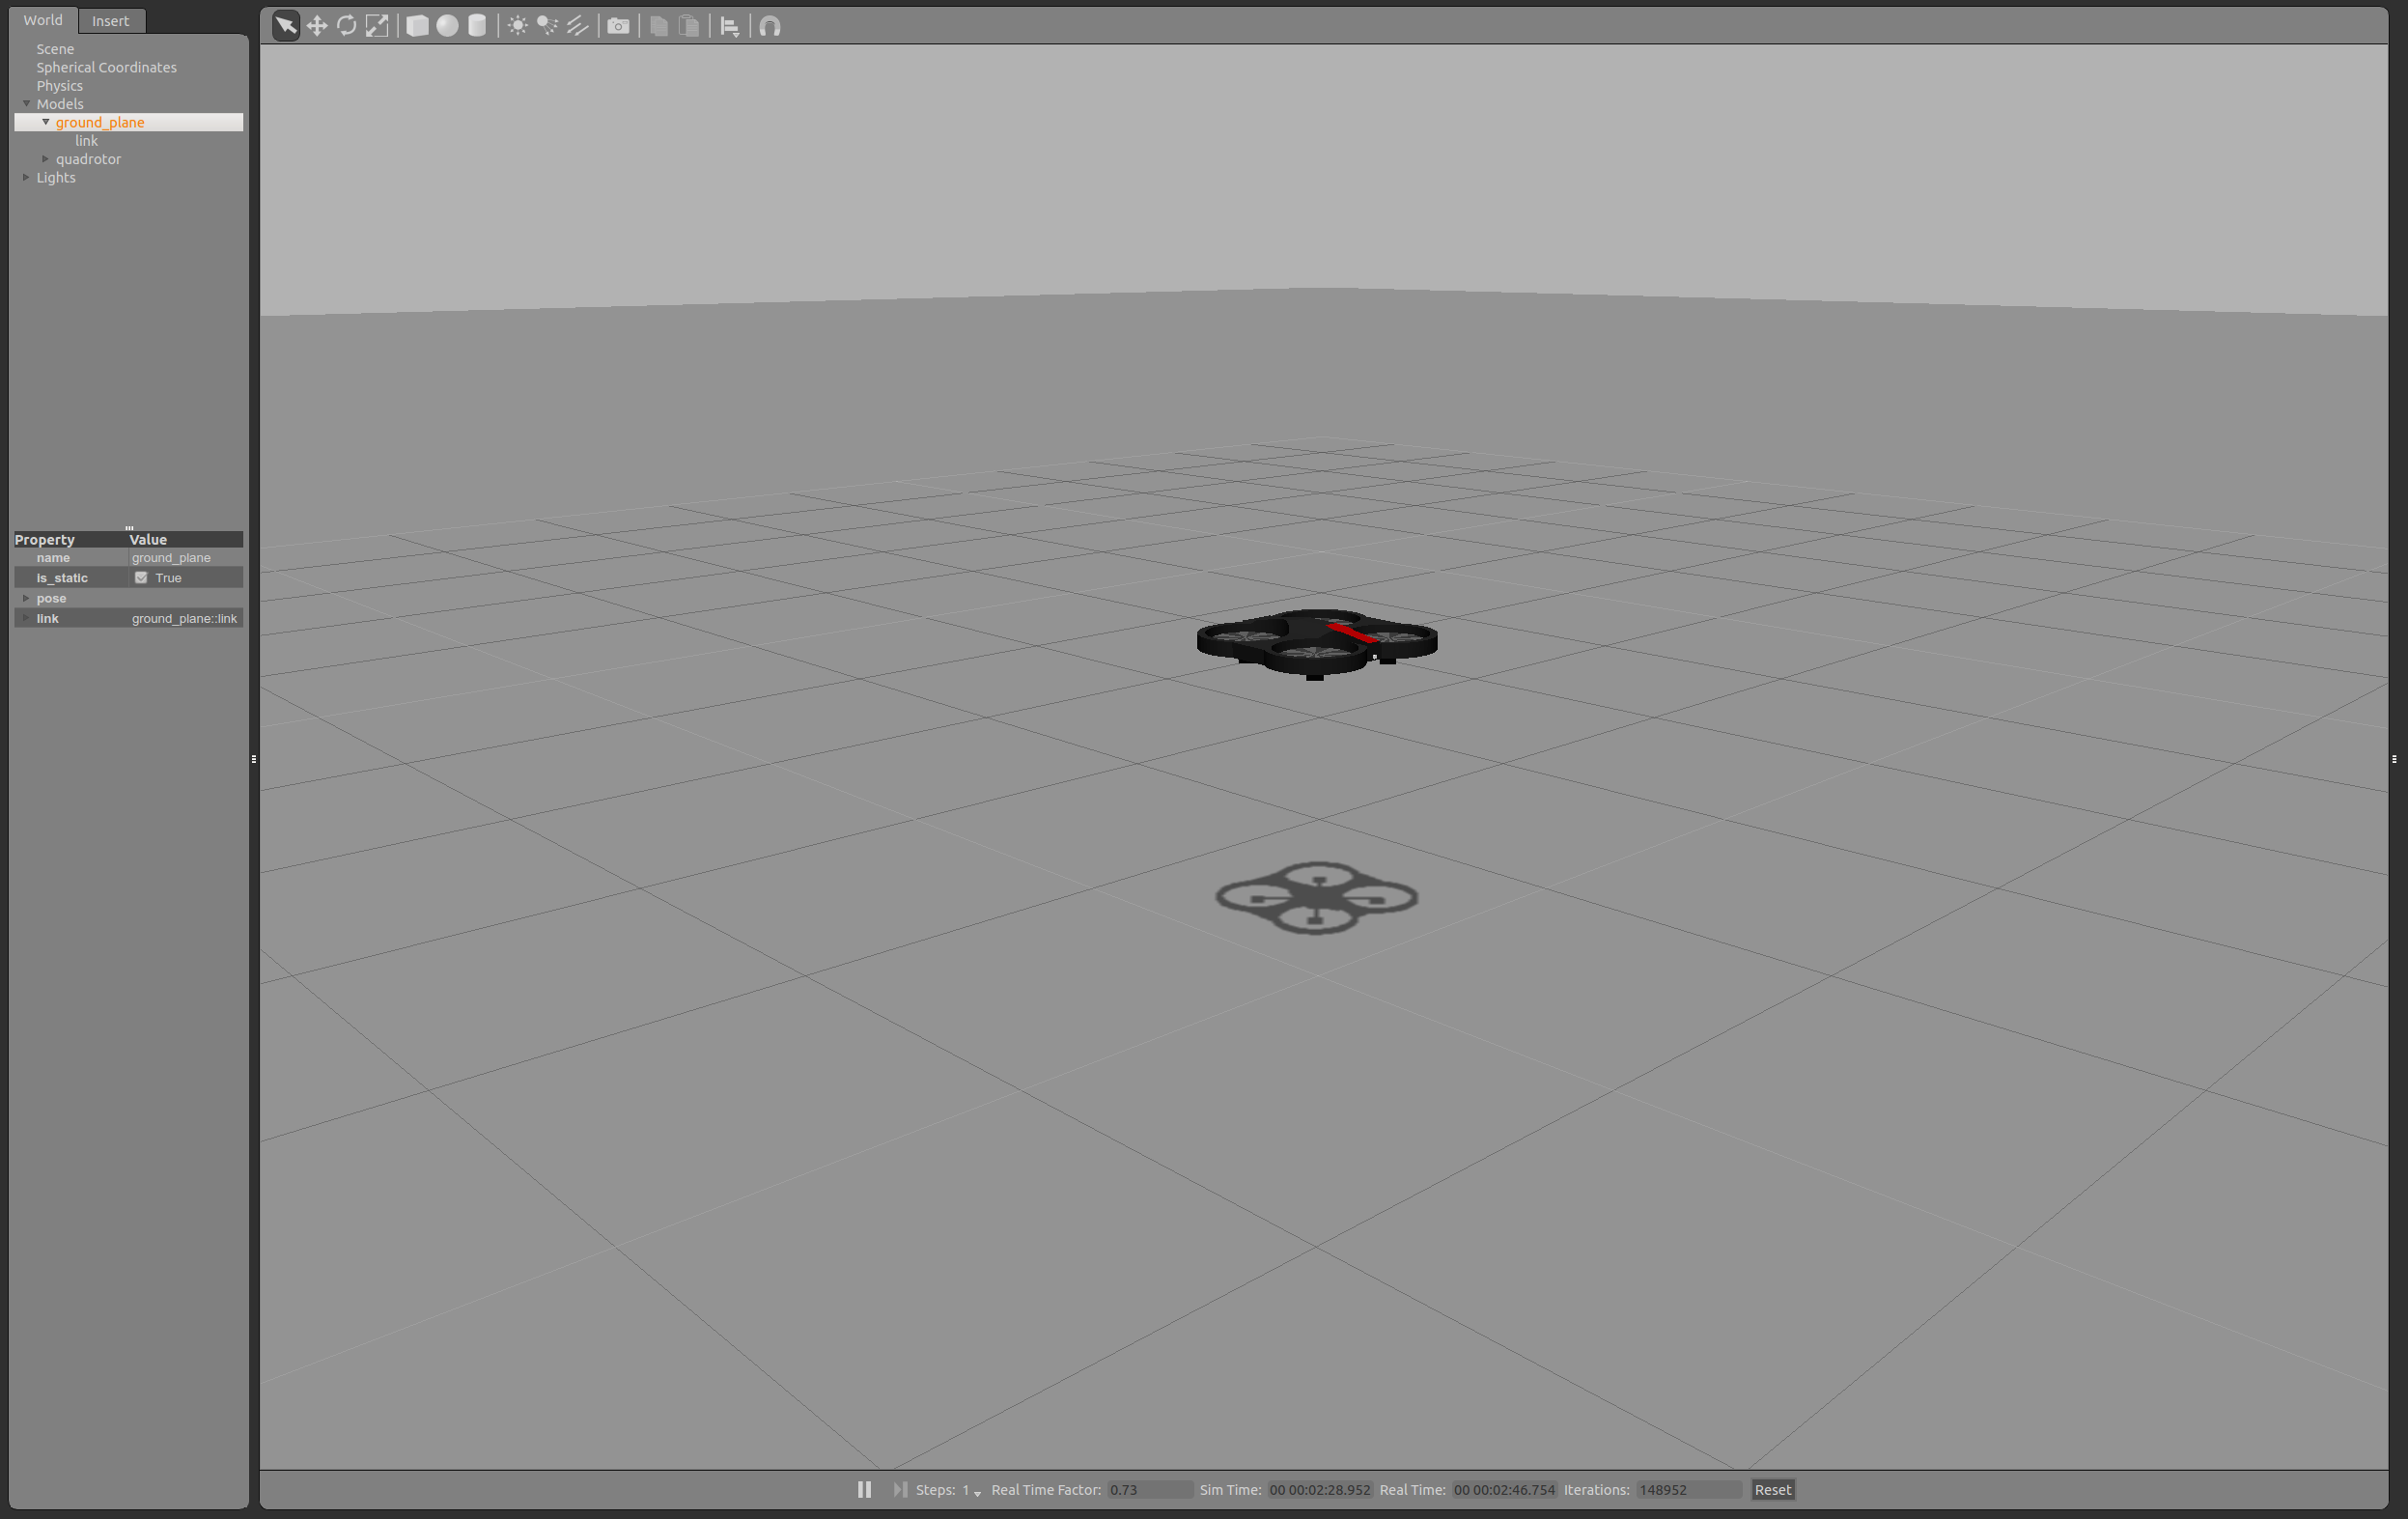
\includegraphics[width=0.8\textwidth]{gazebo}
\caption{Simulador Gazebo}
\label{fig:gazebo}
\end{figure}

Este simulador junto con los plugins, mundos y mapas creados por JdeRobot es una poderosa heramienta que nos será muy útil para nuestro proyecto.

\section{JdeRobot}

JdeRobot es un proyecto desarrollado por el laboratorio de robotica de la Universidad Rey Juan Carlos de Madrid. Es un entorno para el desarrollo de aplicaciones relacionadas con la robotica, la visión artificial, automatización del hogar y escenarios con sensores y actuadores, y software inteligente. Está escrito mayormente en C++ y basado en un entorno de componentes distribuidos. Los componentes, que pueden correr de manera simultánea de manera asíncrona están conectados a través del \emph{middleware} ICE, el cuál veremos a continuación. Los componentes pueden ser escritos en C++, Java, Python... y todos ellos interoperar a través de interfaces ICE.\\

JdeRobot simplifica el acceso a unidades hardware como cámaras. Obtener datos de un sensor es tan sencillo como llamar a una función local, y mandar comandos a un motor o actuar se hace también simplemente llamando a una función local. Estos sensores, actuadores o unidades hardware pueden ser simuladas o reales y estar en local o en una red de datos como internet.\\

Incluye numerosas librerías y herramientas que podemos usar para desarrollar nuestra propia aplicación o para controlar nuestro propio robot. JdeRobot es software libre, bajo licencia GPL y LGPL. También utiliza software de terceros como el simulador Gazebo, ArDroneServer ROS, GTK, OpenCV...\\

La versión utilizada en el proyecto ha sido la 5.3.1, última versión estable en la fecha del comienzo del mismo. Dentro de las herramientas utilizadas en el proyecto hemos hecho uso básicamente de dos:

\begin{itemize}
\item \emph{Plugin de Gazebo}: Desarrollado por JdeRobot para añadir el ArDrone a Gazebo con las mismas funcionalidades al drone real. Este plugin nos permite abstraernos de las conexiones a mas bajo nivel, como la lectura de sensores o en envío de comandos a los motores, simplificando el acceso a los mismo y obteniendo los datos con una simple llamada a función.

\item \emph{ArDroneServer}: Este componente es el encargado de comunicarse directamente con el ArDrone real, ejecutar las funciones y comandos de bajo nivel para obtener los datos y valores de los sensores, y ejecutar las funciones necesarias sobre los motores y actuadores según las órdenes de movimiento dadas. De cara al usuario ofrece seis interfaces ICE, a las que puedes conectar tu aplicación. En la figura \ref{fig:ardroneserver} puedes ver la estructura general del componente.
\end{itemize}

\begin{figure}[htb]
\centering
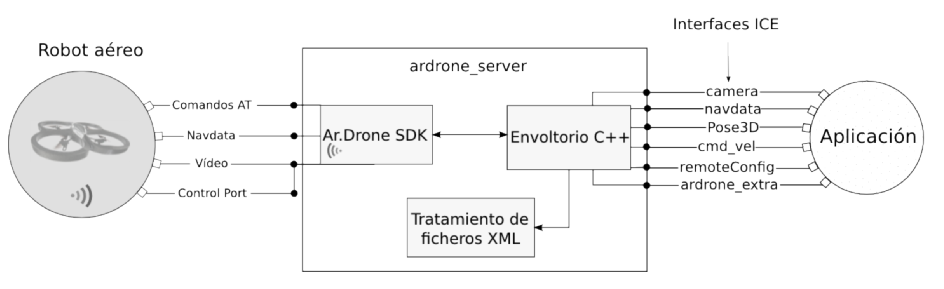
\includegraphics[width=1\textwidth]{ardroneserver}
\caption{Estructura de ArDrone\_Server}
\label{fig:ardroneserver}
\end{figure}

\section{ICE}

ICE o \emph{Internet Communication Engine} es un entorno RPC orientado a objetos desarrollado por Zeroc con soporte para lenguajes como C++, C\#, Java, JavaScript, y Python entre otros, y SO's como Linux, Mac OS X y Windows, que nos permite crear conexiones e interacciones de red entre máquinas con servidores corriendo en diferentes lenguajes y/o SO's. Estas conexiones pueden ser síncronas o asíncronas, usando variedad de protocolos de red como TCP, UDP ó SSL/TTS\\

ICEJS, o ICE for JavaScript es un \textit{plugin} que se le puede añadir a ICE el cual añade la funcionalidad de conexiones mediante \textit{websockets} lo que nos permite conectar navegadores a través de JavaScript a los protocolos mas comunes de ICE. \\

En versiones más actuales ICEJS viene incorporado en la suite principal de ICE, pero nosotros hemos usado la versión 3.5 que es la que soporta la suite de JdeRobot con la que trabajamos, por lo que debemos instalar el plugin una vez instalado ICE.\\

\begin{figure}[htb]
\centering
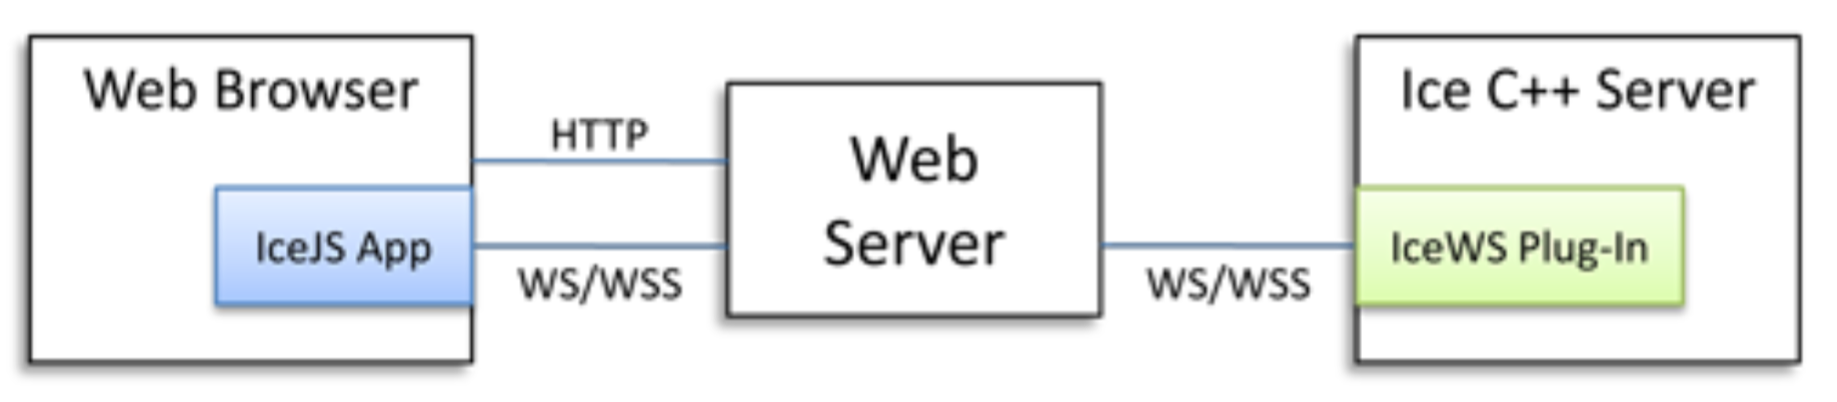
\includegraphics[width=0.8\textwidth]{esquema_icejs}
\caption{Esquema de ICE JS}
\label{fig:esquema_icejs}
\end{figure}

\section{WebRTC}

Web Real-Time Communication (WebRTC) es un proyecto de software libre y gratuito que nos permite tener en el navegador tecnología en tiempo real ('Real-Time Communication' ó RTC), sin plugins, a través de varias APIs de JavaScript. Facilita las llamadas de voz, videollamadas, chat y compartición de archivos y datos. WebRTC es una tecnología entre pares, por lo que nos permite desarrollar estas aplicaciones para que funcionen directamente desde un navegador a otro \emph{sin pasar por servidor intermedio.}\\

En todo el documento nos referimos a una llamada WebRTC entre dos navegadores, lo cual es su principal propósito, pero también está diseñado para que pueda ser integrado con otros sistemas de comunicación como voz sobre IP (VOIP), clientes SIP, e incluso sobre la red telefónica pública conmutada (PSTN).\\

Enviar audio y/o vídeo con calidad, e intercambiar cualquier tipo de datos requiere de muchas funcionalidades complejas en el navegador. Para no preocuparnos de estas dificultades las APIs de WebRTC proporcionan todo el conjunto completo de funciones para manejar y crear nuestras aplicaciones, como el control y administración de la conexión, codificación/decodificación del audio/vídeo, negociación entre navegadores, control de la conexión, atravesar cortafuegos y NAT.\\

Con unas docenas de líneas de JavaScript podemos tener una videoconferencia entre pares con intercambio de archivos o datos en tiempo real. Ese es el potencial que WebRTC tiene. Pero aún así hay una serie de escollos como la señalización, descubrimiento de pares, negociación de la conexión o seguridad que debemos controlar para conseguir una llamada exitosa.\\

Que WebRTC no necesita un servidor no es del todo cierto, ya que sí que necesita de lo que llamamos Servidor de Señalización. Éste es el encargado de establecer el primer contacto entre ellos, facilitando el intercambio de paquetes de la negociación WebRTC.\\

\noindent WebRTC está compuesto de 3 API's:

\begin{itemize}
\item \emph{getUserMedia}: adquisición del flujo local de audio y vídeo.
\item \emph{RTCPeerConnection}: comunicación de audio y vídeo.
\item \emph{RTCDataChannel}: comunicación de cualquier otro tipo de datos.
\end{itemize}

En este momento WebRTC es accesible para todos los usuarios a través de navegadores como Chrome o Firefox. Sin embargo, WebRTC está aún en construcción, tanto la forma de implementar las API's que tiene cada navegador como la propia norma, con sus protocolos de funcionamiento. Como resultado todo lo que exponga sobre estas API's se refiere a la situación actual y puede cambiar en el futuro.\\

A continuación vamos a desgranar y explicar cómo funciona el intercambio de paquetes de señalización así como cada una de las API's que componen WebRTC.\\

\section{WebRTC: Señalización} 
\label{sec:senalizacion}

Señalización es el proceso de intercambio de datos y metadatos necesarios para coordinar una llamada entre navegadores con WebRTC. Para realizar esta labor WebRTC necesita de la ayuda de un servidor externo ya que la norma deja el campo de la señalización a la capa de la aplicación.\\

Los objetivos básicos de la señalización son dos, el intercambios de los datos necesarios para establecer un flujo audiovisual y el intercambio de direcciones de red para que los pares sean alcanzables. Entre las labores para satisfacer estos objetivos se encuentran la detección de los pares, el intercambio de paquetes de control de la sesión como los candidatos \emph{ICE (Internet Communication Engine)} y los \emph{SDP (Session Description Protocol)}, las prestaciones que puede darnos cada par así como cualquier otro dato o paquete necesario para realizar este 'apretón de manos' inicial.\\

WebRTC no especifica qué tipo de servidor hemos de usar para estas funciones. Esto es debido a que diferentes aplicaciones pueden preferir distintos servidores básicos o personalizados según sus necesidades. La única restricción es el uso de la arquitectura JSEP, la cuál especifica cómo debe ser la secuencia de señalización para tener una llamada exitosa.\\


El servidor debe usar la arquitectura \emph{JSEP (JavaScript Session Establishment Protocol)}. Esta arquitectura elimina al navegador de casi todo el flujo de señalización, el cual se maneja desde JavaScript haciendo uso de dos interfaces: transfiriendo los SDP local/remoto e interactuando con la máquina de estados ICE. Esta arquitectura nos evita, entre otras cosas, que el navegador tenga que guardar estados de sesión, de tal manera que se pueden guardar en el servidor y evitar problemas si la página se recarga, por ejemplo. \\

JSEP no establece un modelo particular de señalización más allá de usar uno capaz de realizar el intercambio de los SDP y ICE según la norma RFC3264 de \emph{oferta/respuesta}, [(figura \ref{fig:oferta-respuesta})] de tal manera que ambas partes de la llamada sepan cómo actuar en cada momento. JSEP nos da los mecanismos necesarios para crear estas ofertas, así como aplicarlas a las sesión.\\

\begin{figure}[htb]
\centering
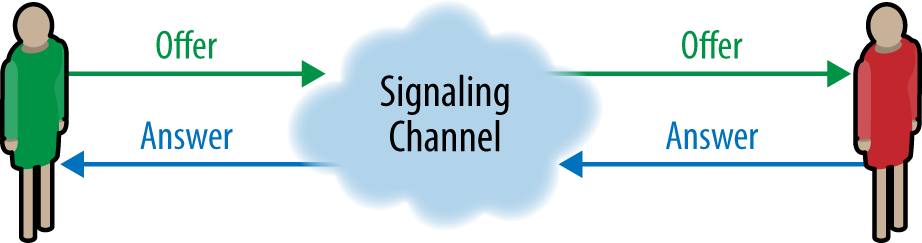
\includegraphics[width=0.9\textwidth]{offer-answer}
\caption{Oferta / Respuesta a través del servidor de señalización}
\label{fig:oferta-respuesta}
\end{figure}


El orden en que se llaman a estos mecanismos o funciones de la API es importante, por lo que la aplicación deberá saber el orden en el que tiene que llamar a cada una, convertir las ofertas en mensajes que entienda el protocolo de señalización elegido y hacer la conversión inversa con los mensajes que se reciben para obtener ofertas que entiendan as API's.\\


\subsection{Estableciendo el Flujo Audiovisual: Descriptores de Sesión y Máquina de Estados}


El manejo de las descripciones de sesión es simple y sencillo. Siempre que el intercambio de una oferta/respuesta es necesario, el par que establece la llamada ó \textit{llamante (callee)} crea la oferta llamando a la función \emph{createOffer()} de la API. Esta oferta puede ser modificada por la aplicación si así fuese necesario y se establece como configuración local en ese par con \emph{setLocalDescription()} y se envía al par remoto a través del servidor de señalización utilizado. Al recibir esta oferta el par \textit{llamado (called)} lo utiliza como configuración del otro par con \emph{setRemoteDescription()} y utiliza \emph{createAnswer()} para crear una respuesta apropiada, la cual establece como configuración local (\emph{setLocalDescription()}) y envía la respuesta de vuelta a través del servidor de señalización. El par llamado al recibir la respuesta llama también a \emph{setRemoteDescription()}, y de esta manera ambos lados tienen la información del descriptor de sesión propio y el del par remoto.\\ 

Para establecer un intercambio de flujo audiovisual, el \textit{agente de usuario (user agent)} del navegador necesita parámetros específicos para indicar al par remoto qué es lo que va a transmitir, de la misma manera que necesita conocer los parámetros del flujo audiovisual que va a recibir para saber cómo decodificarlo y manejarlo. Estos datos se determinan en la descripción de sesión (SDP), los cuales se intercambian en ofertas/respuestas usando las API's JSEP como ya hemos visto anteriormente.\\

Si el SDP pertenece a la parte local o remota tiene su importancia. Una vez realizado el intercambio, cada parte mirará la lista de codecs soportados por él mismo y por la otra parte, y el cruce de los resultados determinará qué codecs debe usar para enviar y cuál para digerir lo recibido. Los parámetros exactos de la transmisión sólo se pueden saber una vez la oferta y la respuesta han sido intercambiados. Sin embargo, hay ocasiones en las que el llamante o el que hace la oferta puede recibir flujo audiovisual después de enviar la oferta pero antes de recibir la respuesta proveniente del otro par. Para procesar este flujo audiovisual de manera adecuada, el manejador del llamante debe conocer los detalles de la oferta antes de que la respuesta llegue.\\

Por lo tanto, para manejar los descriptores de sesión de manera correcta, los agentes de usuario necesitan:

\begin{itemize}
\item Conocer si el descriptor de sesión pertenece a la parte local o remota.
\item Conocer si el descriptor de sesión es una oferta o una respuesta.
\item Permitir a la oferta ser especificada independientemente de la respuesta.
\end{itemize}

Para satisfacer estas premisas JSEP aborda esto añadiendo los métodos \emph{setLocalDescription()} y \emph{setRemoteDescription()} y teniendo un campo en los descriptores de sesión indicando el tipo de sesión que se suministra. En la figura \ref{fig:sdp-oferta-respuesta} podemos ver el esquema de intercambio de paquetes SDP y el ajuste de los mismos en cada par segun corresponde.\\

\begin{figure}[htb]
\centering
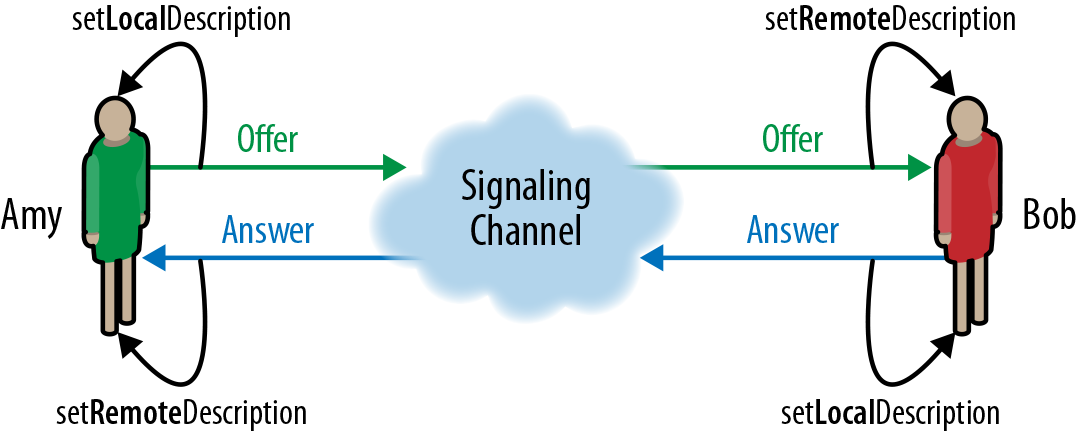
\includegraphics[width=0.9\textwidth]{SDP_offer-answer}
\caption{Intercambio y establecimiento de los SDP en cada par.}
\label{fig:sdp-oferta-respuesta}
\end{figure}

JSEP también permite el uso de respuestas provisionales. Estas respuestas permiten al par remoto o llamado comunicar e informar de los parámetros iniciales de la sesión al llamante, de tal manera que la sesión puede comenzar mientras se espera una respuesta final posteriormente. Este concepto es importante en el modelo oferta/respuesta, ya que al recibir una de estas respuestas el llamante puede liberar y usar más recursos como extra \textit{candidatos ICE, candidatos TURN} o vídeo decodecs. Estas respuestas provisionales no provocan ningún tipo de des-asignación o problema, por lo que pueden ser recibidas a lo largo de la llamada para estabilizar o mejorar la misma según varíen las condiciones del ancho de banda de uno de los pares, por ejemplo.\\


El cometido principal del intercambio de SDP es la negociacion de video. Es un proceso a través del que cada par puede indicar al otro qué resoluciones y \textit{frames rate} de vídeo es capaz de recibir. Esto lo hace a través del atributo \textit{'a=imageattr'} en el SDP. Cada par puede tener límites como la capacidad de proceso que el decoder tiene, o simplemente restricciones de la aplicación.\\


\subsubsection{Formato de los Descriptores de Sesión}

En la especificación WebRTC, los descriptores de sesión o \emph{session descriptions} están formados por mensajes \textit{SDP (Session Description Protocol)}. Este formato no es el más óptimo para manipular con JavaScript, pero es el más popular y aceptado en el campo de las comunicaciones audiovisuales en tiempo real. Este formato es el que usa JSEP para formar e intercambiar los descriptores de sesión.\\

Para facilitar el procesado en JavaScript y una futura flexibilidad, los SDP los genera la API como un objeto o \textit{blob}. Si en un futuro WebRTC soporta algún formato nuevo para los descriptores de sesión, estos serán fácilmente añadidos y habilitados para poder usarlos en nuestras aplicación en vez de SDP.\\

La forma que tiene un paquete SDP es la siguiente:

\begin{lstlisting}[caption=Ejemplo paquete SDP]
v=0
o=- 7729291447651054566 1 IN IP4 0.0.0.0
s=-
t=0 0
a=group:BUNDLE a1 d1
a=ice-options:trickle
m=audio 9 UDP/TLS/RTP/SAVPF 96 0 8 97 98
c=IN IP4 0.0.0.0
a=rtcp:9 IN IP4 0.0.0.0
a=mid:a1
a=msid:QI39StLS8W7ZbQl1sJsWUXkr3Zf12fJUvzQ1
       QI39StLS8W7ZbQl1sJsWUXkr3Zf12fJUvzQ1a0
a=sendrecv
a=rtpmap:96 opus/48000/2
a=rtpmap:0 PCMU/8000
a=rtpmap:8 PCMA/8000
a=rtpmap:97 telephone-event/8000
a=rtpmap:98 telephone-event/48000
a=maxptime:120
a=ice-ufrag:7sFvz2gdLkEwjZEr
a=ice-pwd:dOTZKZNVlO9RSGsEGM63JXT2
a=fingerprint:sha-256 6B:8B:F0:65:5F:78:E2:51:3B:AC:6F:F3:3F:46:1B:35
                     :DC:B8:5F:64:1A:24:C2:43:F0:A1:58:D0:A1:2C:19:08
a=setup:active
a=rtcp-mux
a=rtcp-rsize
a=extmap:1 urn:ietf:params:rtp-hdrext:ssrc-audio-level
a=extmap:2 urn:ietf:params:rtp-hdrext:sdes:mid
a=ssrc:4429951804 cname:Q/NWs1ao1HmN4Xa5

m=application 9 UDP/DTLS/SCTP webrtc-datachannel
c=IN IP4 0.0.0.0
a=mid:d1
a=fmtp:webrtc-datachannel max-message-size=65536
a=sctp-port 5000
a=fingerprint:sha-256 6B:8B:F0:65:5F:78:E2:51:3B:AC:6F:F3:3F:46:1B:35
                     :DC:B8:5F:64:1A:24:C2:43:F0:A1:58:D0:A1:2C:19:08
a=setup:active
\end{lstlisting}



\subsection{Intercambio de los Datos de Red: Interactive Connectivity Establishment (ICE)}

Al igual que los pares tienen que intercambiar información sobre el media, también necesitan hacerlo sobre la información de \textit{red} para que los pares sean visibles entre ellos y puedan alcanzarse. ICE es una técnica usada en aplicaciones de voz, vídeo, \emph{peer-2-peer}, entre otros que nos permite solucionar problemas de alcance de red entre dos ordenadores. Estos problemas son debidos a que los ordenadores suelen estar dentro de una red privada y/o cortafuegos. Esta técnica nos permite descubrir suficiente información sobre la topología de los otros pares para encontrar una o varias rutas potenciales entre ellos.\\

Esta información ha de obtenerse de manera local en cada par con el \textit{Agente ICE} asociado a cada objeto RTCPeerConnection. El Agente ICE es responsable de: 

\begin{itemize}
\item Reunir tuplas candidatas de IP + Puerto.
\item Realizar pruebas de conectividad entre los pares.
\item Enviar \textit{keepalives}.
\end{itemize}

Una vez se ha finalizado y configurado el proceso de descripción de sesión, el Agente ICE local comienza automáticamente el proceso de descubrir todos los posibles candidatos en el par local. Cada candidato posible se le llama \textit{Candidato ICE}:

\begin{enumerate}
\item El Agente ICE pide al sistema operativo las direcciones IP locales.
\item Consulta a un servidor \emph{STUN (Session Traversal Utilities for NAT}) externo la tupla de dirección IP pública y puerto del par.
\item Consulta a un servidor \emph{TURN (Traversal Using Relays around NAT)} como último recurso. 
\end{enumerate}

Como podemos ver, ICE necesita de servidores externos para obtener la tupla de dirección IP y puerto públicos necesarios para el otro par si esta fuera de la misma red local. STUN  es un protocolo estandarizado para descubrir direcciones IP publicas de equipos que están detrás de un NAT. TURN es un servidor para transmitir mensajes entre dos clientes. Este servidor sólo se usará si falla la conexión entre pares después de probar con las direcciones IP locales y las públicas obtenidas en el servidor STUN. No es obligatorio configurar estos servidores. Si la conexión entre los pares es en la misma red no necesitamos configurar servidores STUN/TURN ya que con las direcciones locales es suficiente.\\

\begin{figure}[htb]
\centering
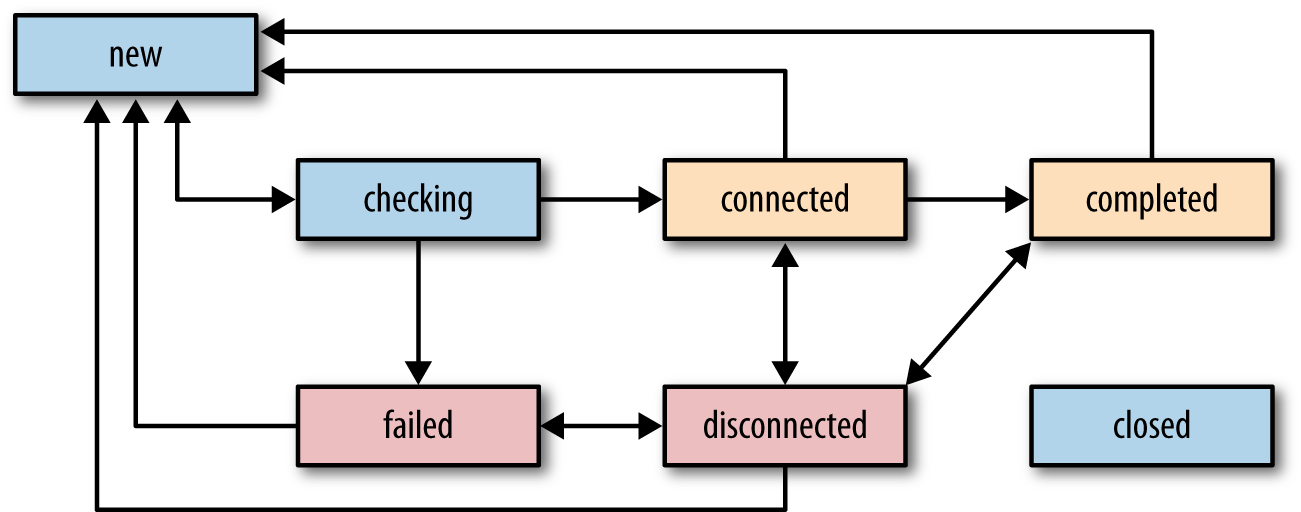
\includegraphics[width=0.9\textwidth]{estados-ICE}
\caption{Maquina de estados y transiciones ICE.}
\label{fig:estados-ice}
\end{figure}

 
Cuando un Candidato ICE es descubierto, se envía al par remoto y una vez allí, se añade en RTCPeerConnection la información de sesión que contiene ese paquete con \textit{setRemoteDescription()}, de tal manera que el Agente ICE puede empezar a hacer pruebas de conectividad para ver si puede alcanzar al otro par.\\

Una vez los dos Agentes ICE tienen una lista completa de los Candidatos ICE de ambos pares, cada agente comprueba pareando ambas lista cuales funcionan. Para ello tienen una planificación de prioridades: primero direcciones IP locales, luego IP públicas y finalmente si ambas fallan servidor TURN. Cada comprobación es una petición/respuesta STUN que el cliente realiza con un particular candidato enviando una petición STUN desde el candidato local al candidato remoto.\\

Si uno de los pares de candidatos funciona, entonces tenemos una ruta de conexión entre ambos pares. Si todos los candidatos fallan ambas conexiones RTCPeerConnection se marca como fallida o la conexión se hace a través de un servidor TURN.\\

Cuando una conexión se ha establecido correctamente cada Agente ICE continua haciendo peticiones STUN periódicas al otro par, lo cual sirve también como \textit{keepalives}.\\

\subsubsection{Goteo de Candidatos ICE \emph{(ICE Candidate Trickling)}}

Recopilar IP's locales es rápido, pero conseguir las IP's publicas con sus puertos a través de servidores STUN requiere de un intercambio de paquetes entre el par y el servidor STUN y por consiguiente más tiempo.\\

\emph{ICE Candidate Tricking} es una extensión del protocolo ICE por la cuál el llamante puede incrementar el número de candidatos para el llamado después de la primera oferta. Este proceso permite al llamado comenzar a establecer las conexiones ICE, sin tener que esperar a que el llamante recopile todos los posibles candidatos. Con esta técnica conseguimos un establecimiento del flujo audiovisual más rápido.\\

Esta técnica es opcional aunque es la recomendada. Las aplicaciones que lo soportan pueden enviar directamente la oferta SDP inicial sin candidatos ICE inmediatamente, y enviar candidatos individuales cuando los vayan descubriendo; las aplicaciones que no lo soportan simplemente esperan la indicación de que la recopilación de candidatos está completa, crean la oferta con todos los candidatos y enviarla.\\

\begin{enumerate}
\item Intercambio ofertas SDP sin Candidatos ICE.
\item Cuando se descubre un candidato se envía directamente a través del servidor de señalización.
\item La comprobación de los Candidatos ICE se realiza en el momento de recibir uno.
\end{enumerate}

\subsubsection{Formato de un Candidato ICE}

\begin{lstlisting}[caption=Ejemplo paquete SDP]
candidate:1 1 UDP 1694498815 192.0.2.33 10000 typ host
\end{lstlisting}

\noindent \textbf{Fundación (1):} Identificador para cada candidato del mismo tipo, misma interfaz y servidor STUN.\\
\textbf{ID (1):} Identificador. 1 para RTP, 2 para RTCP.\\
\textbf{Protocolo (UDP):} Protocolo de transporte del candidato.\\
\textbf{Prioridad (1694498815): }Prioridad del componente dado.\\
\textbf{Dirección IP y puerto (192.0.2.33 10000): }Dirección IP y puerto del candidato.\\
\textbf{Tipo (typ):} Tipo del componente.\\
\textbf{Dirección relacionada (host):} Información opcional que contiene dirección IP y puerto privado.\\


\section{WebRTC: API getUserMedia} 

getUserMedia es la API encargada de suministrarnos el flujo de audio y/o vídeo. Pide permiso al usuario para acceder y utilizar los dispositivos hardware como la cámara y el micrófono. Por el momento sólo está disponible para captar el hardware de audio y vídeo anteriormente mencionado, pero se pretende mejorar y ampliar la API para que en un futuro se pueda hacer \emph{streaming} de casi cualquier fuente de datos, como un disco duro o sensores conectados al ordenador.\\

Para tener una rica videoconferencia no es suficiente con obtener los flujos en crudo \textit{ó formato raw} de la cámara o el micrófono. Cada flujo debe ser procesado para aumentar la calidad, sincronizarlos y ajustar el caudal \textit{(bitrate)} de salida según las fluctuaciones del ancho de banda y la latencia entre pares. A la hora de recibir el flujo nos encontramos en la misma situación pero a la inversa. WebRTC nos da unos motores de procesado de audio y vídeo (figura \ref{fig:audio-video_engines}) que harán todas estas cosas por nosotros.\\

\begin{figure}[htb]
\centering
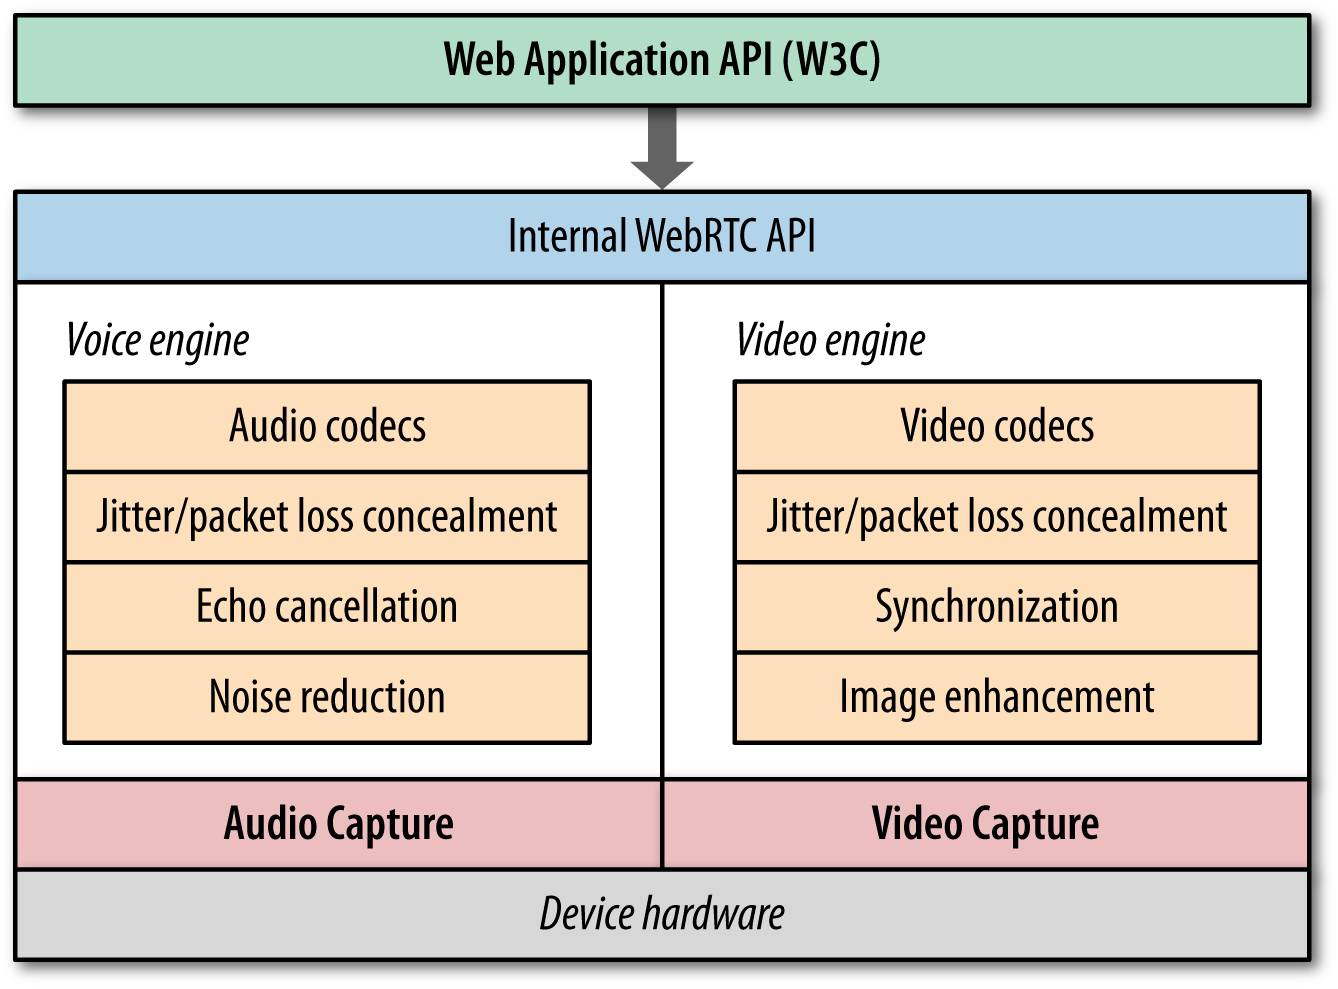
\includegraphics[width=0.9\textwidth]{audio-video_engines}
\caption{Motores de audio y vídeo de WebRTC }
\label{fig:audio-video_engines}
\end{figure}

\emph{getUserMedia} es la API que suministra las funciones y los motores necesarios para poder cumplir con las especificaciones anteriormente mencionadas, así como manipular o procesar los flujos obtenidos. El objeto \textit{MediaStream} (figura \ref{fig:mediaStream}) es la forma en la que nos suministra los flujos esta API.\\

\begin{itemize}
\item El objeto MediaStream consiste en una o varias pistas o \textit{tracks} (\textit{MediaStreamTrack}).
\item Las pistas que componen el MediaStream están sincronizadas una con la otra.
\item La salida del MediaStream puede ser enviada a uno o varios destinatarios, como fuente de vídeo local, un par remoto o procesarlo con funcionalidades que nos proporciona, por ejemplo, HTML5.
\end{itemize}

\begin{figure}[htb]
\centering
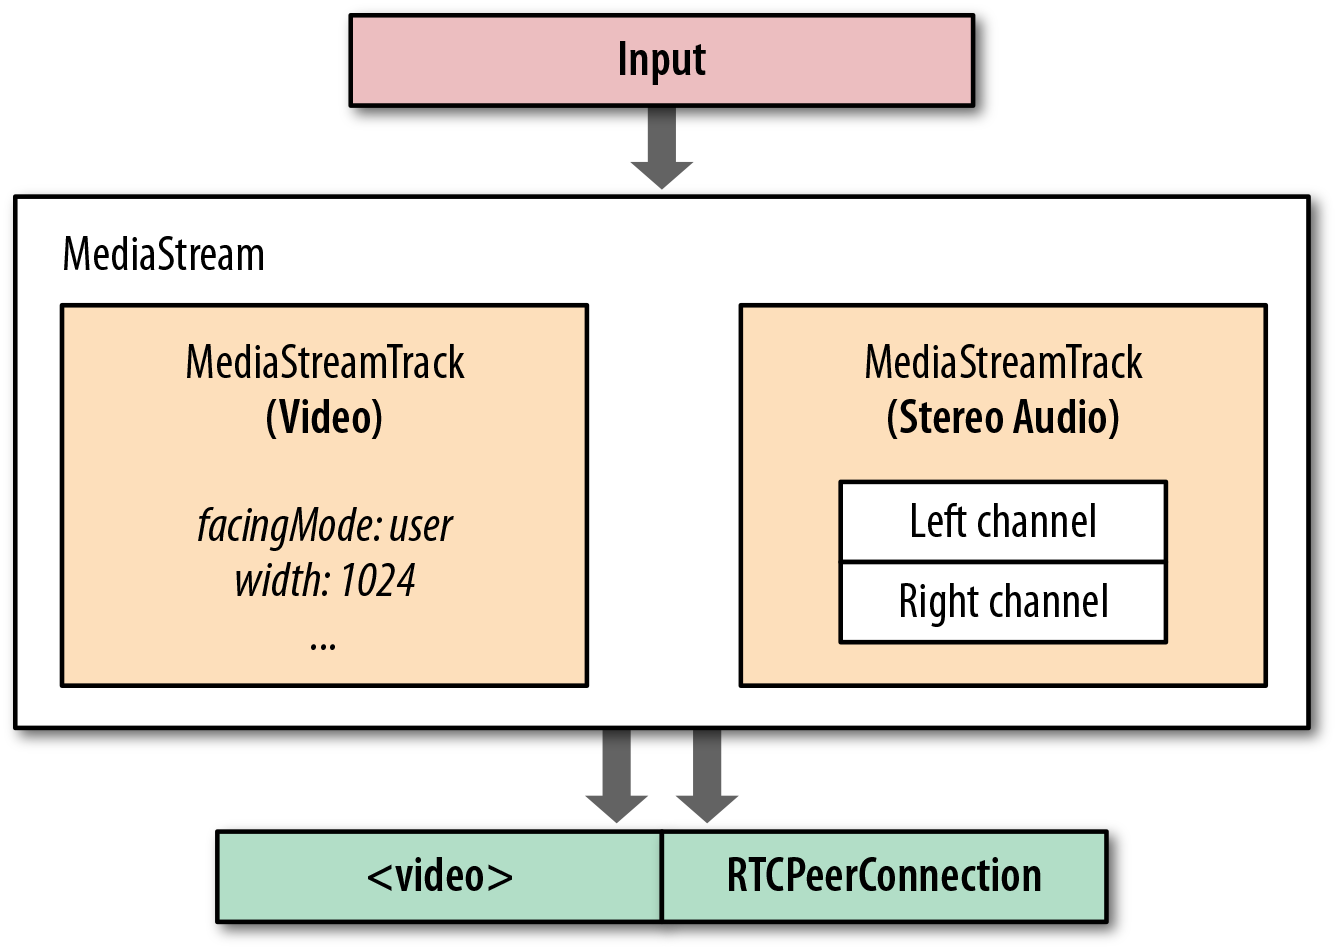
\includegraphics[width=0.9\textwidth]{mediaStream}
\caption{MediaStream}
\label{fig:mediaStream}
\end{figure}

Todo el procesado de audio y vídeo, como la cancelación de ruido, ecualización, mejora de la imagen y todas las demás son automáticamente manejadas por los motores de audio y vídeo.\\

Sin embargo, las características del flujo audivisual son restringidas por las capacidades de los dispositivos de entrada: audio mono o stereo, diferentes resoluciones de vídeo según la cámara, etc. Cuando hacemos una petición de media al navegador, \emph{getUserMedia} nos permite indicar una lista de restricciones obligadas y opcionales.\\

\begin{lstlisting}[caption=Llamada a función RTCPeerConnection]
var constraints = {
    audio: false,
    video: {
        width: { min: 1024, ideal: 1280, max: 1920 },
        height: { min: 576, ideal: 720, max: 1080 },
    }
};

navigator.getUserMedia(constraints, handleUserMedia, handleUserMediaError); 

function handleUserMedia(stream){
    var video = document.querySelector('video');
    video.src = window.URL.createObjectURL(stream);
}

function handleUserMediaError(error){
	console.log('getUserMedia error: ', error);
}

\end{lstlisting}

\section{WebRTC: API RTCPeerConnection}

Esta API es la encargada de crear la conexión \emph{Peer-2-Peer} entre el navegador local y el remoto. Trabaja de manera diferente si es el que hace la llamada (\textit{caller}) y el que la recibe (\textit{called}) debido a la señalización oferta/respuesta que ya hemos visto. Para ello hace uso de sus funciones para completar el proceso de señalización descrito anteriormente.\\

\noindent Es también la encargada de manejar la conexión una vez establecida. Entre las funciones automáticas que realiza se encuentran:\\

\begin{enumerate}
\item Ocultamiento de paquetes perdidos.
\item Cancelación de eco.
\item Adaptación del ancho de banda.
\item Buffer dinámico en función del tembleque (\emph{jitter}) o retardo( \emph{delay}).
\item Control automático de ganancia.
\item Reducción o eliminación de ruido.
\end{enumerate}

Es el desarrollador de la aplicación el encargado de llamar a las funciones que componen esta API en el orden, tiempo y forma correcta para cumplir con la arquitectura JSEP y conseguir un intercambio de descriptores de sesión y de Candidatos ICE exitoso.\\

\noindent La función admite dos argumentos opcionales: 

\begin{lstlisting}[caption=Llamada a función RTCPeerConnection]
var PC = new RTCPeerConnection(ICEconfig, pcConstraints);
\end{lstlisting}

\textit{ICEConfig} es una variable la cuál contiene los datos necesarios para conectarse con el servidor STUN y TURN y poder hacer NAT Trasversal. \textit{pcConstraints} también es una variable a la que se le pueden añadir una serie de restricciones como \textit{RtpDataChannels}, la cuál estará obsoleta en futuras versiones y se dejará de usar. Esta variable está para futuras mejoras.\\

\begin{normalsize}
\noindent \textbf{Protocolos de transporte en tiempo real}\\
\end{normalsize}

El cerebro humano es muy bueno 'rellenando huecos' pero altamente sensible a los retardos. Si perdemos unas muestras de audio o vídeo no nos afecta demasiado en la percepción de lo que estamos recibiendo, pero en cambio añade un retardo al audio con respecto al vídeo y hará que ese material nos sea hasta molesto.\\

Por este motivo las aplicaciones de audio y vídeo en tiempo real están diseñadas para tolerar pérdidas intermitentes de paquetes. Los codecs pueden rellenar estos pequeños espacios que dejan los paquetes perdidos, muchas veces incluso con muy poco impacto con respecto a la imagen real. Una baja latencia y el vicacidad son mucho mas importantes que la fiabilidad (\emph{reliability}).\\

Este requerimiento de vicacidad antes que fiabilidad es la primera razón por la que el protocolo UDP es elegido para el envío de datos en tiempo real. TCP es fiable y tiene entrega ordenada de paquetes. Si uno de ellos se pierde, entonces TCP almacena los paquetes siguientes y para la retransmisión hasta que el paquete perdido es reenviado y recibido. En cambio UDP no garantiza la entrega de paquetes, el orden de entrega, la ruta de los paquetes ni control de congestión de red.\\

WebRTC usa UDP como protocolo de transporte. Dadas las características de UDP, ¿podemos simplemente enviar cada paquete según llega y olvidarnos? no, ya que también necesitamos mecanismos para atravesar NAT's y cortafuegos, negociar los parámetros de cada flujo, encriptar los datos de usuario, congestión de red... Para abastecer estas necesidades WebRTC tiene una lista de protocolos y servicios que trabajan por encima de UDP [(figura \ref{fig:pila_webrtc})].\\

\begin{figure}[htb]
\centering
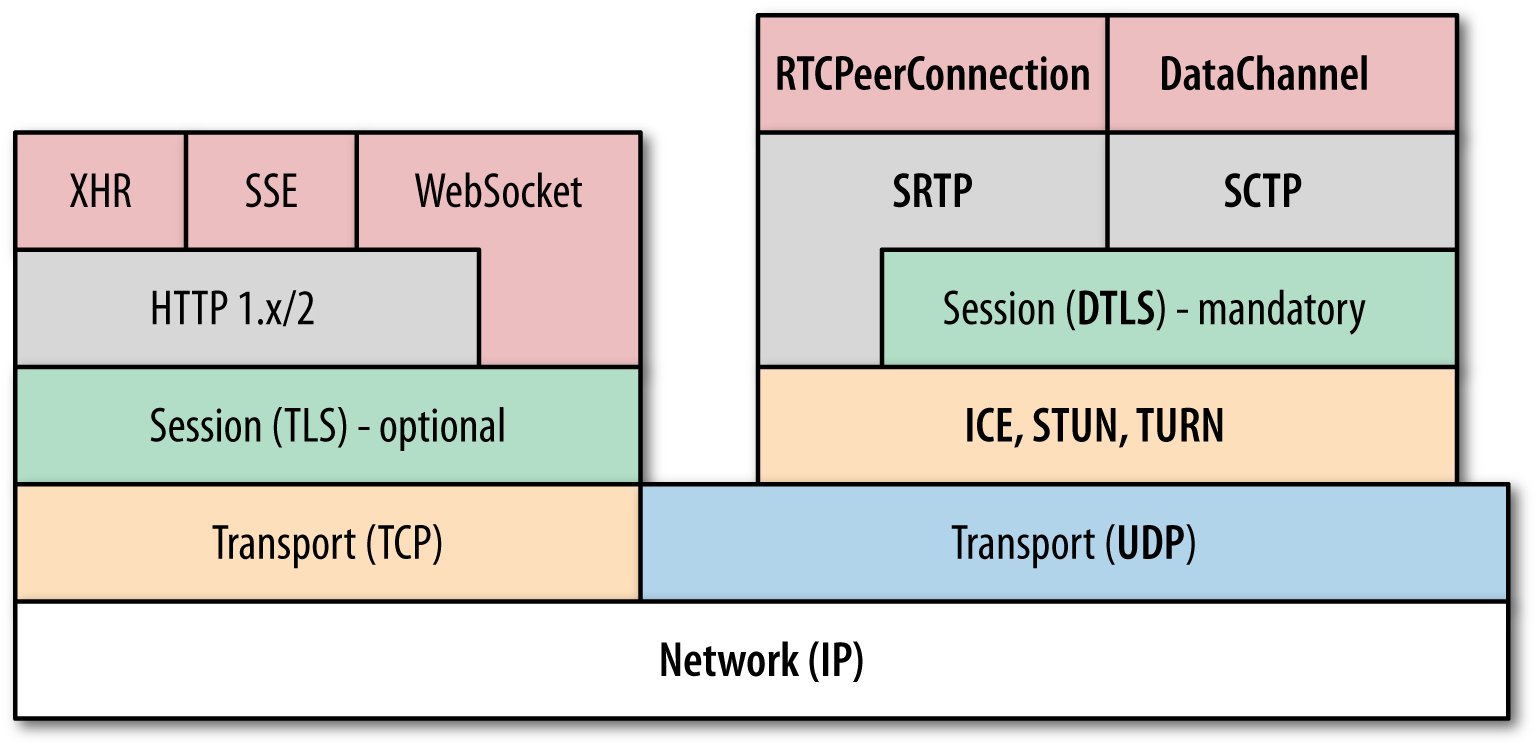
\includegraphics[width=0.9\textwidth]{pila_webrtc}
\caption{Pila de protocolos WebRTC}
\label{fig:pila_webrtc}
\end{figure}


ICE, STUN y TURN son necesarios para establecer y mantener la conexión \emph{Peer-2-Peer} sobre UDP, como ya hemos visto en el apartado de señalización.\\

\begin{normalsize}
\noindent \textbf{Entrega de vídeo con SRTP}\\
\end{normalsize}

WebRTC nos permite adquirir el vídeo/audio y enviarlo para la visualización en el otro par. También nos permite elegir las características con las que queremos adquirir ese vídeo/audio, pero a partir de ahí es WebRTC y el motor de red el que se encarga del resto. Optimización en la codificación, tratar con paquetes perdidos, tembleque, etc, son algunas de las cosas con las que tiene que tratar WebRTC. Por este motivo WebRTC no garantiza la entrega en el otro par del vídeo a su máxima resolución.\\

El motor de red tiene su propio flujo de datos sin tener en cuenta desde el comienzo la capacidad de la red ni el caudal del flujo. Primero empieza enviando el vídeo y el audio a un bitrate bajo (por debajo de 500kbps) y luego comienza a ajustar la calidad del flujo según la capacidad del ancho de banda. Según pueda variar el ancho de banda de la conexión de red así actúa el motor de red para ajustarlo.\\

SRTP define un formato de paquete estándar para enviar audio y vídeo a través de IP, pero por si mismo no proporciona ningún mecanismo o garantías de entrega en orden, fiabilidad en la entrega o corrección de errores. Simplemente encapsula el vídeo y el audio con metadata adicional. Entre esta metadata cada paquete SRTP tiene un numero de secuencia incremental, una marca de tiempo y un identificador SSRC, lo que permite al par que recibe el flujo detectar si los paquetes llegan desordenados, sincronizar los diferentes flujos y asociar cada paquete al flujo correspondiente.\\

SRTP usa un protocolo que lo complementa. Este es SRTCP, el cual es el protocolo que controla el número de paquetes y bytes perdidos, último número de secuencia recibido, \emph{jitter} de los paquetes SRTP recibidos y otras estadísticas. Periódicamente estas estadísticas se intercambian entre los pares y la usan para ajustar la tasa de envío, calidad de codificación y otros parámetros.\\

Ambos protocolos corren directamente sobre UDP y trabajan conjuntamente para adaptar y optimizar la conexión.\\


\section{WebRTC: API RTCDataChannel}

Llegamos a la tercera API de WebRTC. RTCDataChannel nos da la posibilidad de transferir todo tipo de datos u objetos a través de la conexión entre pares establecida con RTCPeerConnection.\\

Esta conexión de datos es \textit{full duplex} y nos permite el intercambio de datos, intercambio de archivos, sincronización de juegos online, etc, todo ello con un retardo mínimo. Las posibilidades son infinitas y se puede adaptar a cualquier necesidad que se tenga para nuestra aplicación.\\

\begin{normalsize}
\noindent \textbf{Capacidades}\\
\end{normalsize}

RTCDataChannel soporta un juego muy flexible de tipos de datos. Soporta \textit{strings}, binarios de JavaScript, \textit{Blobs}, \textit{ArrayBuffer} y \textit{ArrayBufferView}. Según nuestras necesidades nos puede resultar más útil un tipo de datos u otro.\\

Como protocolo de transporte soporta TCP, UDP y SCTP. Esto nos permite configurar la conexión de datos de manera  fiable (\textit{reliable}) o no fiable (\textit{unreliable}). La primera de ellas nos garantiza la entrega de todos los mensajes que enviemos y que los mismos lleguen en el mismo orden que los hemos enviado. Esto provoca una sobrecarga que puede provocar un funcionamiento más lento además de tener un mayola sobrecarga permitiéndonos tener una conexión más rápida. SCTP es un protocolo de transporte similar a TCP y UDP que puede funcionar directamente en la cima del protocolo IP. Sin embargo, en WebRTC, SCTP es construido sobre un túnel DTLS, el cuál corre encima de UDP.

\begin{figure}[htb]
\centering
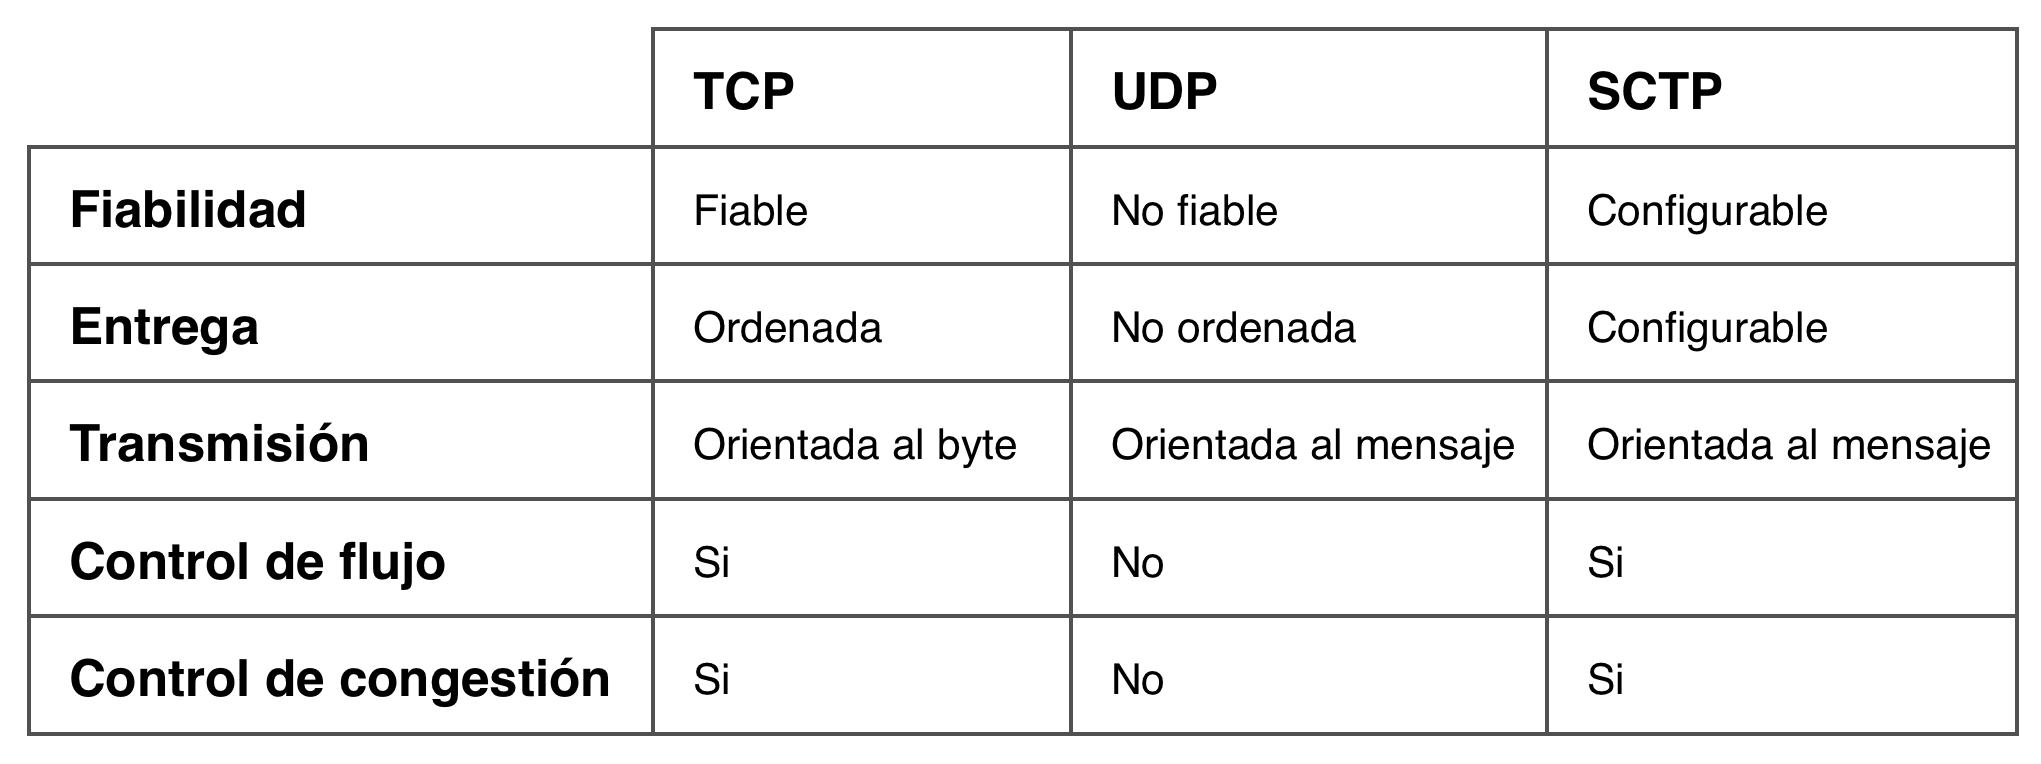
\includegraphics[width=0.9\textwidth]{RTCDataChannel_Capabilities}
\caption{Capacidades de RTCDataChannel.}
\label{fig:datachannel_capabilities}
\end{figure}

\noindent Como las API's anteriores llamamos a RTCDataChannel con una variable con opciones de configuración:

\begin{itemize}
\item \emph{Ordered}: Booleano para indicar si queremos que nos garantice la entrega ordenada de paquetes.
\item \emph{maxRetransmitTime}: Tiempo máximo para intentar retransmitir cada paquete si la entrega falla. (Fuerza el modo no fiable).
\item \emph{maxRetransmits}: Número máximo de veces que queremos que reenvíe cada paquete si la entrega falla. No puede usarse junto con \textit{maxRetransmitTime}. (Fuerza el modo no fiable).
\item \emph{Protocol}: Permite el uso de un subprotocolo pero tiene que ser soportado por TCP/UDP.
\item \emph{Negociated}: Si se configura a verdadero, elimina la configuración automática del \emph{datachannel} en el otro par. Se da por hecho que tienes previsto crear el canal de otra manera con el mismo ID.
\item \emph{Id}: Permite dar tu propio ID al canal.
\end{itemize}

\begin{normalsize}
\noindent \textbf{Seguridad}\\
\end{normalsize}

La encriptación es una obligación para todos los componentes WebRTC. Tanto audio, vídeo, data e información de la aplicación debe estar encriptado cuando se transmite.. En \emph{RTCDatachannel} todos los datos son codificados con \textit{Datagram Transport Layer Security (DTLS)}. DTLS es un derivado de SSL por lo que los datos que intercambies irán igual de seguro que si usásemos SSL. Es obligatorio, para que un navegador pueda usar WebRTC, que tenga implementada esta tecnología.\\


\begin{normalsize}
\noindent \textbf{Entrega de datos con SCTP}\\
\end{normalsize}

Como ya hemos visto en la figura \ref{fig:pila_webrtc}, \emph{RTCDataChannel} trabaja con un protocolo llamado \textit{Stream Control Transmission Protocol (SCTP)}, el cual corre sobre DTLS, y este a su vez corre sobre UDP. Recalco esto ya que a diferencia del audio y el vídeo, para enviar data de la aplicación sí que necesitamos que lleguen todos los paquetes, por lo que si alguno se ha perdido hay que reenviarlo.\\

\noindent WebRTC requiere de 4 características que debe cumplir el protocolo:

\begin{enumerate}
\item El protocolo de transporte debe permitir tener varios canales independientes multiplexados.
\begin{enumerate}
\item Cada canal debe permitir entrega ordenada y desordenada.
\item Cada canal debe tener entrega fiable.
\item Cada canal debe tener niveles de prioridad definidos por la aplicación.
\end{enumerate}
\item El protocolo debe proveer 'orientación al mensaje', por lo que debe tener fragmentación y reagrupacion de los datos.
\item El protocolo debe tener mecanismos control del flujo y de la congestión.
\item El protocolo debe tener seguridad y confidencialidad en los datos que se envían.
\end{enumerate}

La última característica se cumple ya que SCTP corre sobre el túnel DTLS, por lo que los datos que enviemos van encriptados y seguros hasta nuestro destinatario. Por otro lado SCTP, como vemos en la tabla \ref{fig:datachannel_capabilities} permite configurar la fiabilidad y la entrega ordenada de paquetes. SCTP también trocea los datos que queremos enviar y los encapsula en paquetes SCTP de 224 bits.\\

Para el control de flujo y de congestión SCTP tiene un saludo inicial similar al de TCP. Ambos usan la misma ventana inicial de congestión así como la misma lógica de crecimiento y decrecimiento para reducir la congestión una vez la comunicación está activa.\\



\chapter{Desarrollo software}

Una vez nos hemos situado en el contexto en el que se ubica este proyecto, y hemos expuesto los objetivos a cumplir y las herramientas necesarias, nos adentramos a explicar en este capítulo las soluciones desarrolladas para llegar a buen puerto.\\

\section{Diseño}

El escenario que se presenta consta de cuatro elementos principales: el drone, el ordenador a bordo, el ordenador remoto y el usuario humano final. El diseño consta de dos conexiones de tal manera que permitan al usuario final poder teleoperar el cuadricóptero: la primera conexión es entre un navegador web en el ordenador local, el cuál irá a bordo del drone, y el propio drone; la segunda conexión es entre este navegador local y un navegador remoto, dónde se creará una interfaz web amigable y de fácil uso para el control a distancia del drone por parte del usuario final.\\

\begin{figure}[h!]
\centering
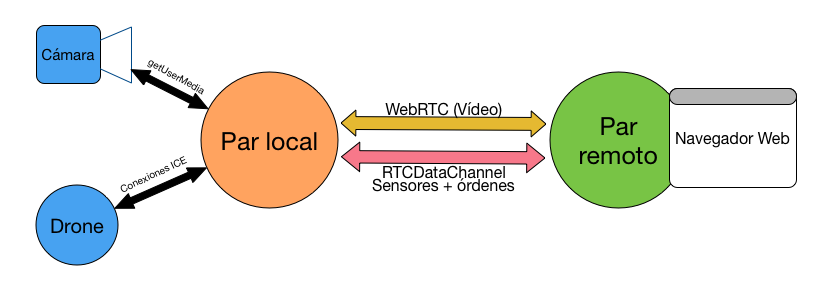
\includegraphics[width=0.9\textwidth]{esquema_general}
\caption{Esquema general del proyecto.}
\label{fig:esquemageneral}
\end{figure}

En la figura \ref{fig:esquemageneral} se representa el esquema general del proyecto con los cuatro actores y las sub-divisiones realizadas. A continuación se expone una vista general a la solución desarrollada para cada uno de esos sub-problemas:

\begin{enumerate}[(a)]

\item \textbf{Conexión local: }consta de dos conexiones: se ha utilizado la API \emph{getUserMedia} de WebRTC para acceder a las imágenes de una cámara que también irá a bordo del drone; por otro lado se ha establecido la conexión entre el drone y el navegador utilizando el plugin ICEJS, el cuál nos permite conectarnos con interfaces ICE a través de \emph{websockets} en el navegador.

\item \textbf{Conexión entre navegadores:} Una conexión punto a punto entre navegadores con la API \emph{RTCPeerConnection} para transferir las imágenes de la cámara, y la API \emph{RTCDataChannel} para transferir los datos de los sensores y las órdenes dadas. 

\item \textbf{Cliente web}: trabaja como transductor para representar los datos recibidos de los sensores del drone y la cámara por un lado, y por el otro de recoger y enviar las órdenes de vuelo dadas por el usuario final.
\end{enumerate}


De manera general en cuanto a la estructura global el par local deberá establecer la conexión con el drone, acceder a sus sensores y actuadores y a la cámara. Deberá también establecer una conexión con el ordenador remoto y enviarle todos estos datos obtenidos del drone. Del par remoto recibirá las órdenes y comandos de movimiento, que deberá enviárselos al drone.\\

El par remoto deberá establecer la conexión con el par local. De éste recibirá todos los datos del drone y deberá representarlos de una manera que el usuario final pueda conocer la situación de vuelo del drone en cada momento. Deberá tener una interfaz amigable que le permita recoger las órdenes de movimiento dadas por el usuario, y enviárselas al par local.\\

Como primer problema se presentó decidir cuál de los dos ordenadores que necesitamos para la conexión WebRTC sería el que realizaría la llamada y en qué momento del flujo. Éste no es un problema trivial, ya que la selección de uno u otro haría que el desarrollo de la aplicación fuese completamente distinto.\\

Se optó por que el par que lleva la batuta de la conexión fuese el ordenador local, ya que éste a su vez también es el encargado de  establecer la conexión con el drone. De esta manera tenemos un par que es el que actuará de maestro, estableciendo ambas conexiones en los momentos oportunos.\\

Como ya se comentó en la sección \ref{sec:senalizacion} el momento en el que se envía y se recibe cada paquete de información es crítico en este sistema de señalización de oferta/respuesta, por lo que el flujo de la comunicación se diseñó y se ha desarrollado como se muestra en la figura \ref{fig:flujodellamada}.\\


\begin{figure}[h!]
\centering
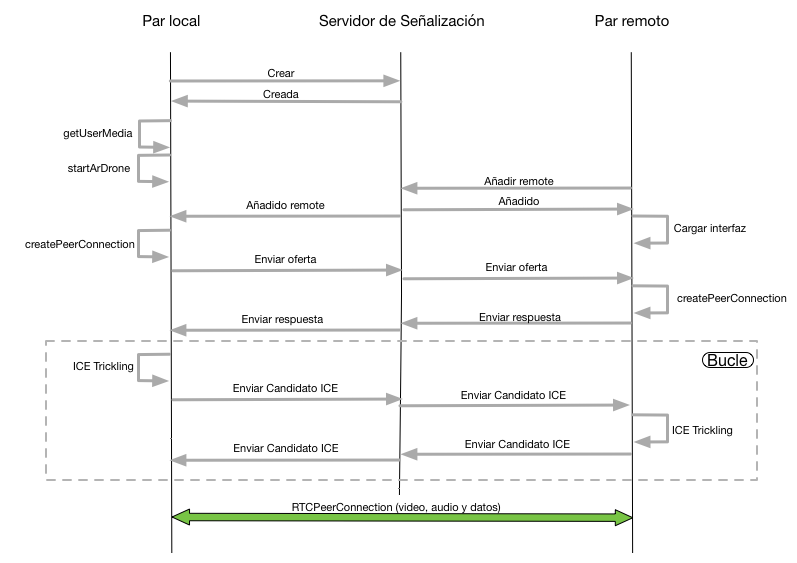
\includegraphics[width=1.1\textwidth]{diagrama_general}
\caption{Flujo de llamada del proyecto}
\label{fig:flujodellamada}
\end{figure}

Como se puede observar el par local es el que lleva la iniciativa de la conexión. En primer término inicia la comunicación con el servidor de señalización. Una vez que éste le contesta afirmativamente a su mensaje de creación de la comunicación inicia un proceso en el que se conecta al cuadricóptero y accede a la cámara. Una vez realizados estos dos procesos espera a que un par remoto quiera unirse a la conexión.\\

Cuando el par remoto accede al servidor de señalización, éste le envía un mensaje al par local indicando que un par remoto se ha conectado. En este momento el par local inicia la creación de la conexión \emph{RTCPeerConection} de WebRTC. Primero se produce el intercambio de paquetes SDP a través del servidor de señalización, y posteriormente el de ICE. Una vez finalizados ambos ya tenemos establecida la conexión WebRTC entre ambos pares.\\

\section{Conexión local drone-navegador}

Esta parte la hemos solucionado dividiendo el problema en dos sub-problemas. Por un lado la conexión con el servidor encargado de conectarse al cuadricóptero, \emph{ardrone\_server}. A través de esta conexión seremos capaces de conectarnos a los elementos, sensores y actuadores del drone. Por otro obtener un flujo de vídeo para poder visualizarlo en la parte remota. Este problema lo hemos solucionado incorporando una cámara a bordo del drone que irá conectada al par local y a la cual accederemos desde el navegador con la API \emph{getUserMedia} que nos brinda WebRTC.\\

Se explica a continuación la conexión con el servidor y posteriormente el acceso a la cámara con \emph{getUserMedia}.\\


\subsection{ArDrone\_server y WebSockets}\label{subsec:ardrone}

Para establecer la conexión con el drone se ha utilizado el componente \texttt{ardrone\_server} de JdeRobot. Este componente son dos piezas. Un plugin en Gazebo para el drone simulado, y el servidor \texttt{ardrone\_server} para el drone real. Estas dos piezas cuentan con las mismas interfaces de conexion ICE por lo que con un único desarrollo es posible utilizar indistintamente tanto la versión simulada con Gazebo como el drone real.\\

Esta conexión se ha divido en dos partes, servidor y cliente. En la parte de servidor se ha tratado su configuración y la activación de \emph{WebSockets} como protocolo sobre el que van mensajes ICE, y la parte del cliente se ha desarrollado desde cero el código \emph{JavaScript} necesario para establecer y controlar la conexión.\\

\subsubsection{Servidor}

Los componentes JdeRobot utilizan, como ya hemos visto, interfaces ICE para el intercambio de información del que se ocupan. Los navegadores no tienen capacidad de usar el \emph{middleware} ICE directamente. Para poder conectarnos con estas interfaces ICE hemos tenido que instalar el plugin ICE for JavaScript, o ICE\-JS. Este plugin nos habilita la opción de conectarnos a estas interfaces directamente desde el navegador usando \emph{websockets}.\\

Aunque estaba disponible la versión 3.6 de ICE\footnote{https://doc.zeroc.com/display/Ice36/Home} la cuál trae en la \emph{suite} instalado de serie ICE\_JS, hemos usado la versión 3.5, ya que es la versión compatible con la versión actual de JdeRobot\footnote{http://jderobot.org/Manual-5}. En esta versión ICE\_JS es un plugin el cuál hay que instalarlo descargando el código fuente desde la página de Zeroc\footnote{https://zeroc.com} y compilarlo.\\

Una vez instalado hay que activar este plugin en el servidor ICE. Para ello hay que añadir la siguiente línea en el archivo de configuración del servidor ICE, en nuestro caso \emph{ardrone\_server}:\\

\begin{lstlisting}[caption=Activación del plugin ICEJS]
# ICE-JS
Ice.Plugin.IceWS=IceWS:createIceWS
\end{lstlisting}

Posteriormentes, en el mismo archivo hay que indicarle las direcciones IP y los puertos de cada interfaz de conexión. Cada conexión se corresponderá con un \emph{WebSocket}, y la nomenclatura es la siguiente:\\

\begin{lstlisting}[caption=Formato \emph{endpoints} de los \emph{WebSocket} de ICEJS]
# ICE-JS
:ws -h ip -p puerto
\end{lstlisting}


El servidor tiene hasta un máximo de seis interfaces diferentes a las que te puedes conectar. Cada una de estas interfaces nos ofrece un servicio diferente. Para nuestro proyecto hemos usado cuatro de esas interfaces:\\

\begin{itemize}
\item \textbf{Pose3D:} Con esta interfaz accedemos a los datos de orientación y posición del cuadricóptero (x, y, z, h y \emph{quaternion}).
\item \textbf{Navdata:} Esta interfaz nos proporciona los datos de navegación procedentes de los sensores, como la velocidad de las componentes (x, y, z) del drone, altitud, la velocidad del viento, el nivel de batería, etc.
\item \textbf{CMDVel:} Esta interfaz es la encargada de recibir las órdenes de movimiento.
\item \textbf{BaseExtra:} Esta interfaz nos da funcionalidades extra como las órdenes de aterrizaje o de despegue del cuadricóptero.
\end{itemize}

Así pues, esta es la forma final que tiene nuestro archivo de configuración:\\

\begin{lstlisting}[caption=Archivo de configuración de ArDrone\_Server.]
# Ice-JS
Ice.Plugin.IceWS=IceWS:createIceWS

# Variables de control para ver traceroutes de las conexiones ICE.
#Ice.Trace.Network = 3
#Ice.Trace.Protocol=1


ArDrone.Pose3D.Endpoints=default -h 0.0.0.0 -p 9998:ws -h 0.0.0.0 -p 19000
ArDrone.Pose3D.Name=ardrone_pose3d

ArDrone.RemoteConfig.Endpoints=default -h 0.0.0.0 -p 9997
ArDrone.RemoteConfig.Name=ardrone_remoteConfig

ArDrone.Navdata.Endpoints=default -h 0.0.0.0 -p 9996:ws -h 0.0.0.0 -p 15000
ArDrone.Navdata.Name=ardrone_navdata

ArDrone.CMDVel.Endpoints=default -h 0.0.0.0 -p 9995:ws -h 0.0.0.0 -p 11000
ArDrone.CMDVel.Name=ardrone_cmdvel

ArDrone.Extra.Endpoints=default -h 0.0.0.0 -p 9994:ws -h 0.0.0.0 -p 17000
ArDrone.Extra.Name=ardrone_extra

ArDrone.NavdataGPS.Endpoints=default -h 0.0.0.0 -p 9993
ArDrone.NavdataGPS.Name=ardrone_navdatagps
\end{lstlisting}

A parte de los \emph{endpoints} es también importante configurar correctamente el nombre de cada uno de las interfaces, ya que será necesario para una correcta conexión desde el navegador. La dirección ip \texttt{0.0.0.0} indica que la dirección de escucha del servidor es la ip local del equipo. Se puede también observar que hemos creado únicamente \emph{WebSockets} para las cuatro interfaces anteriormente descritos.\\


\subsubsection{Cliente}

Una vez configurado el servidor hemos creado el método \texttt{ArDrone.js} en el navegador local, el cuál es el encargado de conectarse y manejar la conexión con el servidor \texttt{ardrone\_server}.\\

Para establecer una comunicación ICE lo primero que se ha creado han sido las variables ICE necesarias. Estas han sido creadas de la siguiente manera:\\

\begin{lstlisting}[caption=Variables para la conexión ICE.]
// Variable ICE para la conexion
var id = new Ice.InitializationData();
id.properties = Ice.createProperties();
id.properties.setProperty("Ice.Trace.Network", "3"); // Propiedad para tracear la conexion
id.properties.setProperty("Ice.Trace.Protocol", "1"); // Propiedad para tracear la conexion
var communicator = Ice.initialize(id);
\end{lstlisting}

Por si fallase la comunicación ICE se le ha añadido a la variable \emph{id} una propiedad con la que podemos seguir la ruta de la comunicación y detectar en qué punto se produce el fallo.\\

Posteriormente es necesario crear una variable que actuará como \emph{proxy}. Es necesario crear una variable por cada interfaz a la que necesitemos conectarnos. Esta es la nomenclatura que sigue:\\

\begin{lstlisting}[caption=Nomenclatura de variable que actuará como \emph{proxy}]
var proxy = communicator.stringToProxy("nombre_interfaz:ws -h " + ip + " -p " + "puerto");
\end{lstlisting}

Nótese en la nomenclatura que donde pone \emph{nombre\_interfaz} se corresponde con el nombre que le hemos asignado al \emph{endpoint} en el archivo de configuración del servidor. Asimismo el puerto también se corresponde con el configurado.\\


La comunicación con las interfaces se realiza mediante el objeto promesa o \emph{promise} de JavaScript. Este objeto se usa para las comunicaciones asíncronas y se caracteriza por tener tres estados: pendiente, cumplida o rechazada. Cuando una promesa ha sido llamada puede presentar el estado cumplida o rechazada, lo que nos permite llamar al argumento correspondiente y poder actuar en consonancia. De esta manera podemos hacer que métodos asíncronos actúen como métodos síncronos.\\

El núcleo de la conexión con el servidor \emph{ardrone\_server} queda como sigue:\\
\newpage
\begin{lstlisting}[caption=Núcleo ArDrone]
// base extra connection
var baseextra = communicator.stringToProxy("ardrone_extra:ws -h " + ip + " -p " + baseextraPort);
jderobot.ArDroneExtraPrx.checkedCast(baseextra).then(
    function(ar){
        extraProxy = ar;
        console.log("extraProxy connected: " + ar);
    },
    function(ex, ar){
        console.log("extraProxy NOT connected: " + ex);
    }
);               

// NavData
var basenavdata = communicator.stringToProxy("ardrone_navdata:ws -h " + ip + " -p " + navdataProxyPort);
jderobot.NavdataPrx.checkedCast(basenavdata).then(
    function(ar){
        console.log("navdataProxy connected: " + ar);
        navdataProxy = ar;
        navdataProxy.getNavdata().then(
        function(navdata){
            if (navdata.vehicle == ARDRONE_SIMULATED) {
                virtualDrone = true;
                console.log("virtualDrone = true");
            } else {
                virtualDrone = false;
                console.log("virtualDrone = false");
            }
        },
        function (ex, ar){
            console.log("Fail getNavdata() function: " + ex);
        }
        );
    },
    function (ex, ar){
        console.log("navdataProxy NOT connected: " + ex);
    }        
);        

// CMDVelPrx
var basecmdVel = communicator.stringToProxy("ardrone_cmdvel:ws -h " + ip + " -p " + cmdVelProxyPort);
jderobot.CMDVelPrx.checkedCast(basecmdVel).then(
    function(ar){
        console.log("cmdVelProxy connected: " + ar);
        cmdVelProxy = ar;
    },
    function(ex, ar){
        console.log("cmdVelProxy NOT connected: " + ex);
    }
);             

// Pose3D
var basepose3D = communicator.stringToProxy("ardrone_pose3d:ws -h " + ip + " -p " + pose3DProxyPort);
jderobot.Pose3DPrx.checkedCast(basepose3D).then(
   function(ar){
       console.log("pose3DProxy connected: " + ar);
       pose3DProxy = ar;
        window.po = pose3DProxy;
        resolve("Stuff worked!");
       pose3DProxy.getPose3DData().then(
           function (ar){
               console.log("getPoseDData().");
               pose = ar;
           },
           function(ex, ar){
               console.log("Fail call getPoseDData().");
           });
   },
   function(ex, ar){
       console.log("pose3DProxy NOT connected: " + ex)
   }
);
\end{lstlisting}

Tenemos cuatro promesas con sus respectivos argumentos de éxito o fallo, una para cada interfaz ICE. Las variables que nos devuelven los argumentos de éxito se guardan en las variables correspondientes de cada interfaz \texttt{(extraProxy, navdataProxy, cmdVelProxy, pose3DProxy)}. Estas variables son importantes ya que son las que utilizaremos en las funciones manejadoras que se explican a continuación.\\

En este punto ya estamos conectados con las interfaces del servidor, y por consiguiente, con el drone. Para poder teleoperar el drone hay que crear unas funciones que serán los manejadores. Por un lado hemos creado las funciones en JavaScript de aterrizaje y de despegue. Estas funciones utilizan la interfaz \emph{ardrone\_extra}:\\

\begin{lstlisting}[caption=Funciones aterrizaje y despegue.]
// extraProxy functions  
function takeoff() {
    extraProxy.takeoff().then(
        function(ar){
            console.log("Take Off.");
        },
        function(ex, ar){
            console.log("Take Off failed.")
        }
     );
}
    
function land() {
        extraProxy.land().then(
        function(ar){
            console.log("Landing.");
        },
        function(ex, ar){
            console.log("Landing failed: " + ex)
        }
     );
}
\end{lstlisting}

Ejecutar estas órdenes en el drone se realiza en JavaScript también con el objeto promesa, con sus respectivos argumentos de éxito o error en la ejecución de la misma.\\

Las interfaces ICE \emph{Navdata} y \emph{Pose3D} son las encargadas de suministrar todos los datos de navegación de los sensores. Las funciones JavaScript con las que accedemos a estas interfaces y actualizamos todos estos datos son las siguientes:

\begin{lstlisting}[caption=Variables actualización datos de los sensores.]
function updateNavData() {
    navdataProxy.getNavdata().then(
        function(ar){
            navdata = ar;
            //console.log("updateNavData()");
        },
        function (ex, ar){
            console.log("Fail getNavdata() function." + ex)
        }        
    );    
}

function updatePose(){
    pose3DProxy.getPose3DData().then(
            function (ar){
                pose=ar;
                //console.log("getPose3DData. ")
            },
            function(ex, ar){
                console.log("Fail call getPoseDData(): " + ar);
            });   
}
\end{lstlisting}


Llamando a estas funciones periódicamente tenemos actualizados en todo momento los datos de navegación procedentes de los sensores: brújula, posición, velocidad, altitud...\\

Para poder teleoperar el drone se ha implementado una función que es la encargada de enviarle las órdenes de movimiento. Estas órdenes nos llegan desde el par remoto a través de la conexión entre nevagadores que explicaremos con mas detenimiento más adelante.\\

\begin{lstlisting}[caption=Función manejadora de las órdenes.]
function sendVelocities () {
    cmdVelProxy.setCMDVelData(cmd).then(
        function(ar){
          //console.log("sendVelocities.");
        },
        function(ex, ar){
          console.log("sendVelocities failed.")
        }
    );
}
\end{lstlisting}

Esta función admite una variable como argumento, (\emph{cmd}) la cuál contiene los parámetros que recibimos del drone. Esta variable es una variable CMDVel de JdeRobot y tiene esta estructura:\\

\begin{lstlisting}[caption=Variable CMD]
var cmd = new jderobot.CMDVelData; 
cmd.linearX=0.0;
cmd.linearY=0.0;
cmd.linearZ=0.0;
cmd.angularZ=0.0;
cmd.angularX=0.0;
cmd.angularY=0.0;
\end{lstlisting}

Contiene seis parámetros que son las velocidades lineales X, Y, Z y las angulares en los mismos ejes. Estas velocidades pueden variar desde 0.0 hasta 1.0 en intervalos de 0.1.\\


\subsection{getUserMedia}

La interfaz que no hemos utilizado de las que nos ofrece el servidor \texttt{ardrone\_server} es la interfaz \emph{cameraserver}. Esta interfaz se encarga de recoger las imágenes de la cámara integrada en el drone. La razón por la que no usar la interfaz del drone que accede a la cámara es que queríamos utilizar la tecnología que nos brinda WebRTC con drones, y esto incluye el acceso a una cámara con la API \emph{getUserMedia}. Esta cámara se conecta a nuestro ordenador local a través de una conexión USB. Cámara y MiniPC van a a bordo del drone.\\

Como WebRTC aún no es una norma, para acceder a la cámara desde cualquier navegador debemos crear una variable que sea compatible con todos los que tengan implementado las APIs de WebRTC. Para ello hay que añadirle los prefijos correspondientes de cada navegador:\\


\begin{lstlisting}[caption=Variable de getUserMedia.]
navigator.getUserMedia = navigator.getUserMedia || navigator.webkitGetUserMedia || navigator.mozGetUserMedia;
\end{lstlisting}


Acceder a la cámara  con \emph{getUserMedia} se hace a través de una función que admite tres argumentos. El primer argumento que admite la función es una variable en la que le indicamos las restricciones que queremos: audio, vídeo, solo uno de ellos, resoluciones... Las configuraciones para nuestro proyecto son las siguientes:\\

\begin{lstlisting}[caption=Restricciones de getUserMedia]
var constraints = {
    audio: false,
    video: {
        width: { ideal: 1280, max: 1920 },
        height: {ideal: 720, max: 1080 },
    }
};
\end{lstlisting}

Sólo accedemos al vídeo de la cámara, ya que el audio no lo necesitamos para el proyecto. Por otro lado indicamos una resolución ideal, de 1280x720 píxeles. Si la cámara que le conectamos al ordenador tiene más capacidad restringimos su resolución a HD (1920x1080 píxeles).\\

Los siguientes dos argumentos son dos llamadas de vuelta o \emph{callbacks}. El primero es el callback de éxito, y el segundo el de error. Según sea de exitoso el acceso a la cámara se llamará a una función u otra. Si nos devuelve éxito se llama a una función con la que guardaremos el flujo y lo visualizaremos en un elemento vídeo de HTML5. Esta visualización que se produce en el par local no es necesaria pero se ha incluido para tenerlo como referencia a la hora de realizar los experimentos. Si devuelve error mostramos en el terminal del navegador un mensaje del error ocurrido.\\

\begin{lstlisting}[caption={getUserMedia.}, label={lst:getusermedia}]
// Manejador de exito
function handleUserMedia(stream){
	localStream = stream;

	if (window.URL){
		localVideo.src = window.URL.createObjectURL(stream);
	} else{
		localVideo.src = stream;
	}
}

// manejador de error
function handleUserMediaError(error){
	console.log('getUserMedia error: ', error);
}

//Funcion getUserMedia
navigator.getUserMedia(constraints, handleUserMedia, handleUserMediaError); 
\end{lstlisting}

El flujo que nos proporciona \emph{getUserMedia} y el cuál guardamos en la variable \emph{localStream} (línea 3 del listado \ref{lst:getusermedia}) será el que enviemos al par remoto con la API \emph{RTCPeerConnection}. Este punto lo veremos en la sección \ref{subsec:transmisionvideo}.\\

\section{Conexión entre navegadores}

Interconectar el ordenador remoto al drone a través del ordenador local es el segundo de los objetivos marcados. Para ello vamos a utilizar WebRTC por su comunicación entre pares sin necesidad de utilizar servidores intermedios.\\

Este objetivo se ha divido en tres sub-objetivos como siguen:
\begin{itemize}

\item \emph{Visualización en remoto de cámara a bordo:} La conexión tiene que ser capaz de transportar el flujo audiovisual de la cámara del drone desde el navegador local hasta el navegador remoto.

\item \emph{Sensores de navegación.} Los datos obtenidos de los sensores de navegación del cuadricóptero como la brújula, el GPS, altímetro... deberán ser enviados al ordenador remoto donde se visualizarán.

\item \emph{Órdenes}. Desde el ordenador remoto deberán enviarse hacia el ordenador local las órdenes dadas para el aterrizaje, despegue, y comandos de movimiento.

\end{itemize}

Para desarrollar la conexión multimedia entre los navegadores con la tecnología WebRTC lo primero que se ha desarrollado ha sido el servidor de señalización.\\

\subsection{Servidor de señalización}

Las necesidades a cubrir en cuanto al servidor de señalización es que sea capaz de intercambiar los datos de red necesarios (Candidatos ICE) y de paquetes SDP. El intercambio debe hacerse con el protocolo de oferta/respuesta según lo establecido en la arquitectura JSEP explicada con anterioridad.\\

Se ha optado por desarrollar el servidor escrito sobre \emph{Node.js}\footnote{https://nodejs.org/}. Las razones por las que hemos elegido este servidor es que está escrito en JavaScript, por lo que nos resulta muy útil al utilizarse el mismo lenguaje de programación que vamos a utilizar para el resto del proyecto. Por otro lado es un servidor muy liviano.\\

Para cumplir con la arquitectura JSEP vamos a utilizar la librería \emph{Socket.io}\footnote{http://socket.io}, la cuál nos facilita el desarrollo de aplicaciones con necesidades de conexión entre equipos a través de \emph{Websockets}.\\

Como se puede ver en la figura \ref{fig:flujodellamada}, el servidor recibe cuatro tipos de paquetes diferentes. Cuando se conecta el par local, cuando se conecta el par remoto, intercambio de candidatos ICE e intercambio de SDP. Sabiendo que tanto los candidatos ICE como los paquetes SDP son objetos, decidimos crear el servidor aceptando tres tipos diferentes de paquetes: el inicial del par local, el inicial del par remoto, y mensajes genéricos que contendrían los objetos anteriormente mencionados. Así pues, esta es la forma del código que gestiona en el servidor el intercambio de paquetes para la señalización.\\

\newpage
\begin{lstlisting}[caption=Núcleo servidor de señalización]
io.sockets.on('connection', function (socket){

	// Manejador de mensajes genericos 'message' (intercambios SDP y Candidatos ICE)
	socket.on('message', function (message) {
		//log('Server --> got message: ', message);
		// Si el que envia es Droner hay que mandarlo al remote
		if (socket.id == dronerID) {
			io.sockets.socket(newPeer).emit('message', message);
		// Si el que envia es remote hay que mandarselo al droner
		} else if (socket.id== newPeer) {
			io.sockets.socket(dronerID).emit('message', message);
		} 
	});

	// manejador de mensjes 'create'  enviados por Droner
	socket.on('create', function () {
		//log('Server --> Droner has sido conectado');
		socket.join();
		dronerID = socket.id;
		socket.emit('created');
	});
	

	// Manejador de mensajes 'join remote ' enviados por remote
	socket.on('join remote', function () {
		//log("Server --> Un 'remote' se ha unido.");
		
		io.sockets.in().emit('join remote');
		socket.join();
		newPeer = socket.id;
		socket.emit('joined');
	});
});
\end{lstlisting}

Una vez tenemos el servidor operativo vamos a explicar cómo se ha creado la conexión entre pares y cómo se ha usado esta conexión para transmitir el vídeo de la cámara y los datos de los sensores del drone hasta el par remoto.\\

\subsection{RTCPeerConnection: Transmisión de vídeo}\label{subsec:transmisionvideo}

La conexión entre pares se crea en el momento en el que el par local recibe del servidor de señalización un mensaje indicando que el par remoto se ha conectado y está preparado para establecer la conexión. En ese momento se ejecuta una función que configura los parámetros necesarios y  crea la comunicación.\\

Al igual que en \emph{getUserMedia} debemos configurar las variables necesarias para que sean compatibles con todos los navegadores. Para establecer la conexión necesitamos tres variables distintas:\\


\begin{lstlisting}[caption=Variables WebRTC]
RTCPeerConnection = window.RTCPeerConnection || window.mozRTCPeerConnection || 
                       window.webkitRTCPeerConnection || window.msRTCPeerConnection;
RTCPSessionDescription = window.RTCSessionDescription || window.mozRTCSessionDescription ||
                       window.webkitRTCSessionDescription || window.msRTCSessionDescription;
RTCIceCandidate = window.RTCIceCandidate || window.mozRTCIceCandidate ||
                        window.webkitRTCIceCandidate || window.msRTCIceCandidate;
\end{lstlisting}


\begin{itemize}
\item \emph{RTCPeerConnection}: Esta variable es la encargada de crear y mantener la conexión entre pares. Esta variable necesitará de las otras dos para crear la conexión.
\item \emph{RTCPSessionDescription}: Crea los SDP locales y se encarga de gestionar los SDP recibidos.
\item \emph{RTCIceCandidate}: Encargada de descubrir los Candidatos ICE y de gestionar los recibidos del otro par.
\end{itemize}


También debemos indicarle los servidores STUN y TURN a los que conectarse para averiguar los pares de IP y puerto para los Candidatos ICE:\\

\begin{lstlisting}[caption=Servidores STUN y TURN]
var ICE_config = {
  'iceServers': [
    {
      'urls': 'stun:stun.l.google.com:19302'
    },
    {
      'urls': 'stun:23.21.150.121'
    },
    {
      'urls': 'turn:192.158.29.39:3478?transport=udp',
      'credential': 'JZEOEt2V3Qb0y27GRntt2u2PAYA=',
      'username': '28224511:1379330808'
    },
    {
      'urls': 'turn:192.158.29.39:3478?transport=tcp',
      'credential': 'JZEOEt2V3Qb0y27GRntt2u2PAYA=',
      'username': '28224511:1379330808'
    }
  ]
};
\end{lstlisting}

Una vez tenemos las variables configuradas, la forma en la que creamos la conexión WebRTC es la siguiente:\\

\begin{lstlisting}[caption=RTCPeerConnection.]

var PeerConnection = new RTCPeerConnection(ICE_config, pc_constraints);
\end{lstlisting}

Esta función admite dos argumentos. El primero es la configuración ICE que acabamos de ver y el segundo es una variable con las restricciones de todas las funcionalidades y configuraciones que tiene \emph{RTCPeerConnection}. En nuestro caso esa variable está vacía ya que la configuración por defecto es más que adecuada para nuestros intereses.\\

Para el intercambio de paquetes en la señalización es necesario crear los manejadores que \emph{RTCPeerConnection} necesita para los SDP y para los Candidatos ICE. El par local tiene sus manejadores ya que es el encargado de llevar la batuta de la conexión, y el par remoto tiene otros manejadores diferentes. \\

Los SDP se manejan en el par local con el método \emph{createOffer} que al ser llamado activa el proceso de crear la oferta SDP. Cada vez que crea uno nuevo salta un evento en la función que se le ha indicado, llamada \emph{gotLocalDescription}. Esta función se encarga de ajustar el SDP local al SDP que se acaba de crear y de mandárselo al otro par a través del servidor de señalización. Si al crear un SDP se produce un error se llama a la función de error, la cual se encargará de notificarlo en la consola del navegador.\\


\begin{lstlisting}[caption={Manejador de los SDP.}, label={lst:manejadorsdp}]
// Funcion de exito
function gotLocalDescription(sessionDescription){
  PeerConnection.setLocalDescription(sessionDescription, successLocalSDP, errorLocalSDP);
  sendMessage(sessionDescription);
}

// Funcion de error
function onSignalingError(error){
  console.log('Fallo al crear el SDP: ' + error);	
}

// Metodo manejador de las SDP
PeerConnection.createOffer(gotLocalDescription, onSignalingError);
\end{lstlisting}

Esta oferta es recibida en el par remoto a través del servidor de señalización y se guarda como la oferta del otro par, ya que la necesitaremos para conocer las características del flujo audiovisual que nos llegará:\\


\begin{lstlisting}[caption={Estableciendo SDP del par remoto.}]
PeerConnection.setRemoteDescription(new RTCPSessionDescription(message));
\end{lstlisting}

Al establecer el SDP remoto ocurre un evento del método \emph{createAnswer} y crea una respuesta a la oferta recibida.\\

\begin{lstlisting}[caption=Manejador de respuestas SDP]
PeerConnection.createAnswer(gotLocalDescription, onSignalingError);
\end{lstlisting}


Las funciones de éxito y error \emph{gotLocalDescription} y \emph{onSignalingError} son las mismas que en el otro par, puedes encontrarlas en el listado \ref{lst:manejadorsdp}.\\

Para manejar los Candidatos ICE utilizamos el método manejador \emph{onicecandidate}, el cuál llama a la función indicada, \emph{handleIceCandidate()} en nuestro caso, en el momento en que se encuentra un Candidato ICE. Esta función se encarga de enviar el candidato a través del servidor de señalización. Ambos pares usan este mismo evento con la misma configuración en la detección y envío de candidatos ICE.\\

\begin{lstlisting}[caption=Manejador de los Candidatos ICE locales.]
function handleIceCandidate(event){
  //console.log('handleIceCandidate event: ', event);
  if (event.candidate) {
    sendMessage({
    type: 'candidate',
    label: event.candidate.sdpMLineIndex,
    id: event.candidate.sdpMid,
    candidate: event.candidate.candidate});
  } else {
    console.log('End of candidates.');
  }
    // console.log('Local ICE candidate: \n' + event.candidate.candidate);
  
}

// Metodo manejador de candidatos ICE
PeerConnection.onicecandidate = handleIceCandidate; // Manejador ICE local (manda ICE local a remoto)
\end{lstlisting}

Los candidatos son recibidos en ambos pares a través del servidor de señalización. Se crea el candidato y se le añade como candidato remoto con el método \emph{addIceCandidate}.\\

\begin{lstlisting}[caption=Manejador de los Candidatos ICE remotos.]
var candidate = new RTCIceCandidate({sdpMLineIndex:message.label,candidate:message.candidate});
PeerConnection.addIceCandidate(candidate);
\end{lstlisting}


Uno de los puntos mas importantes para el proyecto que se tiene que encargar \emph{RTCPeerConnection} es transferir el flujo visual desde el par local al par remoto. WebRTC nos lo permite de una forma muy sencilla. En el par local, con un método al que le añadimos como argumento el flujo que hemos obtenido al llamar a la API \emph{getUserMedia}:\\

\begin{lstlisting}[caption=Manejador del flujo audiovisual en el par local.]
PeerConnection.addStream(localStream); 
\end{lstlisting}

Y en el par remoto con un método manejador llamado \emph{onaddstream}, que en el momento en el que salta el evento llama a la función \emph{handleRemoteStreamAdded}, y ésta se encarga de configurar el flujo en una etiqueta vídeo de HTML5.\\

\begin{lstlisting}[caption=Manejador del flujo audiovisual en el par remoto.]
// Funcion manejadora
function handleRemoteStreamAdded(event) {

    var remoteVideo = document.getElementById("droneVideo"); // 

	if (window.URL){
		remoteVideo.src = window.URL.createObjectURL(event.stream);
	} else{
		remoteVideo.src = event.stream;
	}
    //console.log('Remote stream attached!!.');
	remoteStream = event.stream;
}

// Metodo manejador 
PeerConnection.onaddstream = handleRemoteStreamAdded;
\end{lstlisting}

Una vez creada y establecida la conexión \emph{RTCPeerConnection} la usaremos para crear la conexión de datos \emph{RTCDataChannel}, para transportar toda la información necesaria en ambas direcciones.\\


\subsection{RTCDataChannel}

\emph{RTCDataChannel} nos permite transferir cualquier tipo de dato u objeto entre los pares a través de la comunicación creada por \emph{RTCPeerConnection}. Hemos usado esta API para transferir tanto los datos obtenidos de los sensores del drone (del navegador local al navegador remoto) como las órdenes de movimiento dadas (deo navegador remoto al navegador local).\\

Para crear esta conexión basta con llamar al método \emph{createDataChannel()} de \emph{RTCPeerConnection} en el par local ya que es quien arranca la conexión. Este método admite dos argumentos, el primero es el nombre que le damos a esta conexión y el segundo es un objeto en el que se especifica la configuración de las propiedades disponibles. La única propiedad que se ha configurado distinta de las que vienen por defecto es la entrega ordenada de paquetes, estableciéndolo en falso, ya que de esta manera introduce menos retraso a la comunicación, eliminando cuellos de botella ya que el medio en el que se transfieren los paquetes no es ruidoso ni tiene condiciones extremas para que se produzcan demasiadas pérdidas de paquetes.\\

\begin{lstlisting}[caption=Establecimiento conexión RTCDataChannel en el par local.]
// Creacion de la comunicacion dataChannel
dataChannel = PeerConnection.createDataChannel("droneDataChannel", {ordered: false});

// Metodo de error para la creacion del dataChannel
dataChannel.onerror = function (error) {
  console.log("Data Channel Error:", error);
};\end{lstlisting}

Si en el momento de crear la conexión ocurre un error salta un evento en el método \emph{onerror} que nos comunica a través de la terminal el error concreto que se ha producido.\\

Para el control de la comunicación RTCDataChannel utiliza tres métodos para gestionar la conexión. Por un lado los métodos de inicio y final de la conexión creada, y el método que maneja los mensajes recibidos.\\

\begin{lstlisting}[caption={Manejadores de RTCdataChannel.}, label={lst:manejadoresdatachannel}]
function handleReceiveChannelStateChange() {
  var readyState = dataChannel.readyState;
  if (readyState == closed) {
    isChannelRunning = false;
    clearInterval(intervalo); //Paramos el intervalo de actulizacion con el drone si el canal se cierra
  }
}

dataChannel.onopen = handleReceiveChannelStateChange;
dataChannel.onclose = handleReceiveChannelStateChange;
dataChannel.onmessage = handleMessage;
};\end{lstlisting}

La función \emph{handleMessage} es la encargada de manejar los mensajes recibidos, pero hablaremos en profundidad de ella más adelante.\\

En el par remoto para establecer la conexión RTCDataChannel hemos configurado el método \emph{ondatachannel}. Este método se encarga de unirse a la comunicación creada por el par local con las mismas propiedades y configuraciones que se le han indicado. Cuando se activa este método llama a la función \emph{gotReceiveChannel} que es la encargada de manejar  la conexión. Esta función se encarga de configurar la conexión en la variable local, y de establecer en los métodos de apertura y cierre de la comunicación las funciones manejadoras. Las función manejadora \emph{handleSendChannelStateChange} es la misma que la mostrada en el listado \ref{lst:manejadoresdatachannel}.\\

\begin{lstlisting}[caption={Establecimiento de RTCDataChannel en el par remoto.}]
function gotReceiveChannel(event) {
	dataChannel = event.channel; // Establece el datachannel
	dataChannel.onopen = handleSendChannelStateChange;
	dataChannel.onclose = handleSendChannelStateChange;
	dataChannel.onmessage = handleMessage;
}

// Evento manejador al recibir apertura comunicacion datachannel del par local.
PeerConnection.ondatachannel = gotReceiveChannel;
};\end{lstlisting}

Una vez establecida la comunicación de datos \emph{RTCDataChannel} podemos enviar los datos a través del método \emph{dataChannel.send()} y recibirlos con el método manejador \emph{onmessage}. A continuación vamos a ver cómo hemos utilizado estos métodos para enviar y recibir los sensores del drone y las órdenes de movimiento.\\


\subsubsection{Sensores de navegación}

Los datos de los sensores los recogemos en el par local. Llamamos a una función del método ArDrone, explicado en la sección \ref{subsec:ardrone}, que a su vez llama a las funciones que se conectan directamente con las interfaces ICE de \texttt{ardrone\_server} para recoger los datos. Esta llamada la hacemos de manera periódica con una función \emph{setinterval()} de JavaScript.\\

\begin{lstlisting}[caption=Intervalo actualización y envío de datos de los sensores.]
intervalo = setInterval(arDrone.updateAndSend, 15);
\end{lstlisting}

Después de actualizar los datos, esta función a su vez llama a la función \emph{sendNavigationData(pose, navdata)} que es la encargada de enviar estos datos a través de la conexión \emph{RTCDataChannel}. Esta función admite dos argumentos, el primero es el objeto \emph{pose}, que contiene los datos recogidos de la interfaz \emph{Pose3D}, y el segundo el objeto \emph{Navdata}, con los datos de navegación recogidos de la interfaz \emph{Navdata}.\\

\begin{lstlisting}[caption=Envio de los datos de los sensores en el par local.]
function sendNavigationData(pose, navdata) {
	var s = {pose:pose, navdata:navdata};
	dataChannel.send(JSON.stringify(s));
	//console.log("Send navigationData.");
}
};\end{lstlisting}

Para enviar los datos al navegador remoto primero creamos un objeto JavaScript, en el que introducimos los objetos \emph{Pose} y \emph{Navdata}. Este objeto lo transformamos a un objeto JSON\footnote{http://www.json.org} para enviarlo por el canal de datos \emph{RTCDataChannel}.\\

Los datos llegan al par remoto en forma de evento a la función \emph{handleMessage()}.\\

\begin{lstlisting}[caption=Manejo de los datos de los sensores en el par remoto.]
function handleMessage(event) {
    var data = JSON.parse(event.data);
    pose = data.pose;
    navdata = data.navdata;
}
\end{lstlisting}

Esta función se encarga de reconvertir el objeto JSON recibido a objeto JavaScript, y posteriormente guardamos los objetos \emph{pose} y \emph{navdatas} para su posterior representación en pantalla. Estos datos los visualizaremos en unos relojes de navegación, los cuáles estudiaremos con más detalle en la sección \ref{subsec:relojesnavegacion}.\\


\subsubsection{Órdenes de movimiento}\label{subsec:ordenes}

El par remoto es el encargado de transferir las órdenes dadas por el usuario al par local, y éste a su vez al drone. El usuario tiene distintas maneras de introducir o hacer saber al equipo las órdenes que quiere dar. Una de ellas es a través de unos \emph{joysticks} multidispositivo situados en las esquinas inferiores de la pantalla, y la otra mediante un mando conectado por USB al ordenador.\\

En la sección \ref{subsec:joysticks} se analizarán en profundidad ambos, mientras que en esta sección nos centraremos en el intercambio de los datos.\\

La forma en la que hemos diseñado la interfaz hace que tengamos dos joysticks, uno de ellos controla la dirección y velocidad del drone, y el otro controla la altitud y el giro del drone. A parte de esto tenemos otro tipo de órdenes, las llamadas especiales, que son la orden de despegue y la orden de aterrizaje. Por este motivo se han creado tres tipos de funciones de envío:\\

\begin{lstlisting}[caption=Funciones de envío de órdenes en el par remoto.]
function enviarOrden(d){
    //console.log(d);
    var data = {orden:d};
    dataChannel.send(JSON.stringify(data));
}

function sendCMDVel(x, y){
    var data = {x:x,y:y};
    //console.log(data);
    dataChannel.send(JSON.stringify(data));
}

function sendAltYaw(alt, yaw){
    //console.log(d);
    var data = {alt:alt, yaw:yaw};
    dataChannel.send(JSON.stringify(data));
}
\end{lstlisting}

La función \emph{enviarOrden()} es llamada al pulsar un botón de despegue o aterrizaje que implementaremos en la interfaz de usuario. En esta función creamos un objeto JavaScript con la orden, le reconvertimos a un objeto JSON y se envía a través del canal RTCDataChannel con \emph{dataChannel.send(JSON.stringify(data));}.\\


\emph{sendCMDVel()} es llamada cuándo el usuario interactúa con el \emph{joystick} situado en la parte inferior izquierda de la pantalla. Esta función admite como argumento el valor de las componentes espaciales \emph{x} e \emph{y}. Creamos un objeto JavaScript y lo enviamos de la misma forma que el resto de datos que enviamos a través del canal RTCDataChannel.\\

Con el segundo \emph{joystick} situado en la esquina inferior derecha controlamos la altitud y el giro del drone. La función \emph{sendAltYaw()} también admite dos argumentos, la altura (o componente espacial \emph{z}) y el giro del drone. Enviamos de la misma manera, creando una variable JavaScript con ellas, reconvertimos a objeto JSON y enviamos \emph{dataChannel.send()}.\\

Todos estos datos los recibimos en el par local con la función \emph{handleMessage()}. En esta función reconvertimos el objeto JSON a objeto JavaScript y llamamos a la función manejadora \emph{handleReceiveData()} a la que le enviamos como argumento el objeto JavaScript.\\

\begin{lstlisting}[caption=Manejo de las órdenes recibidas en el par local.]
// Manejador de datos recibidos 
function handleReceiveData(data) {
  if ("orden" in data) {
    if (data.orden == "takeoff") {
      arDrone.takeoff();
    } else if (data.orden == "land") {
      arDrone.land();
    } else {
      console.log("Orden no valida. ");
    }
  } else if ("x" in data) {
    arDrone.setXYValues(data.x, data.y);
  } else if ("alt" in data) {
    arDrone.setAltYaw(data.alt, data.yaw);
  } else {
    console.log("Dato invalido. ");
  }		
}

// Recibimos los paquetes del datachannel y los enviamos al manejador de datos
function handleMessage(event) {
  //console.log('Received message: ' + event.data);
  var data = JSON.parse(event.data);
  handleReceiveData(data);
}
\end{lstlisting}


La función manejadora se encarga de discernir qué tipo de dato ha llegado y llamar a la función correspondiente del módulo ArDrone.\\

En este punto tenemos toda la comunicación de datos entre pares terminada, por lo que procedemos a explicar el desarrollo de la interfaz web de usuario.\\

\section{Interfaz web de usuario en cliente remoto}

El diseño de la interfaz se ha diseñado con tecnologías web de ultima generación que nos permiten teleoperar el drone de una forma fácil, sencilla e intuitiva.\\

Esta interfaz está compuesta principalmente por cuatro ingredientes: la visualización del vídeo recibido del navegador remoto a pantalla completa, unos \emph{joysticks} virtuales para el manejo del drone complementados con un mando físico, unos relojes de navegación que nos representarán los datos recibidos de los sensores del drone y una visualización espacial en 3D del drone.\\

\subsection{Visualización del vídeo}

Para teleoperar el drone de una manera efectiva necesitamos poder visualizar el vídeo que recibimos de la cámara de la mejor manera posible. Hemos optado por visualizarlo a pantalla completa en el navegador, por debajo del resto de elementos que tendremos en la pantalla. Este tipo de representación es especialmente útil cuándo se ejecuta en un teléfono móvil o en una tableta.\\

Para situar el vídeo a pantalla completa primero necesitamos definir en la hoja de estilos o \emph{CSS} el cuerpo de la página con margen cero, y posteriormente situar el vídeo en el centro de la pantalla y con tamaño 100\%. Para el tiempo que transcurre entre que se inicia el período de señalización hasta que recibimos el vídeo se establece una imagen de fondo\\

\begin{lstlisting}[caption=Vídeo a pantalla completa.]
body{
       background: url(background.jpg) no-repeat;
       background-size: 100% 100%;
}

video#droneVideo { 
       position: fixed;
       top: 50%;
       left: 50%;
       min-width: 100%;
       min-height: 100%;
       width: auto;
       height: auto;
       z-index: -100;
       -webkit-transform: translateX(-50%) translateY(-50%);
       transform: translateX(-50%) translateY(-50%);
       background: url(background.jpg) no-repeat;
       background-size: cover; 
}
\end{lstlisting}

En la figura \ref{fig:interfazweb} se puede observar el vídeo procedente de la cámara mostrándose de fondo por debajo del resto de elementos de la interfaz.\\

\subsection{Joysticks y Gamepad}\label{subsec:joysticks}

Para que el usuario controle el drone hemos optado por desarrollar dos opciones. La primera opción es a través de unos \emph{joysticks} situados en la pantalla, los cuáles son multidispositivo, ya que se pueden usar en un ordenador con el puntero del ratón y en dispositivos táctiles con los dedos. Por otro lado, también puede ser controlado con un mando USB conectado en el ordenador.\\

\subsubsection{Joysticks virtuales}

Los joystick han sido desarrollados como un canvas de HTML5 en el que dibujamos un círculo y un aro exterior.\\

\begin{lstlisting}[caption=Aro y círculo del joystick.]
function dibujarAro(x, y, r) {
        ctx.beginPath();
        ctx.arc(x, y, r, 0, 2 * Math.PI, true);
        ctx.lineWidth = 7;
        ctx.strokeStyle = "rgb(87,125,25)";
        ctx.stroke();
}

function dibujarCirculo(x, y, r) {
        ctx.beginPath();
        ctx.fillStyle = "rgb(75, 144, 176)";
        ctx.arc(x, y, r, 0, 2 * Math.PI, true);
        ctx.fill();
}
\end{lstlisting}


El aro exterior es un elemento fijo, es decir no se mueve y lo utilizamos como "tope" para el círculo interior. El círculo es móvil según los movimientos del usuario. En la figura \ref{fig:joysticks} podemos ver la apariencia final de los dos \emph{joysticks}.\\

\begin{figure}[h!]
\centering
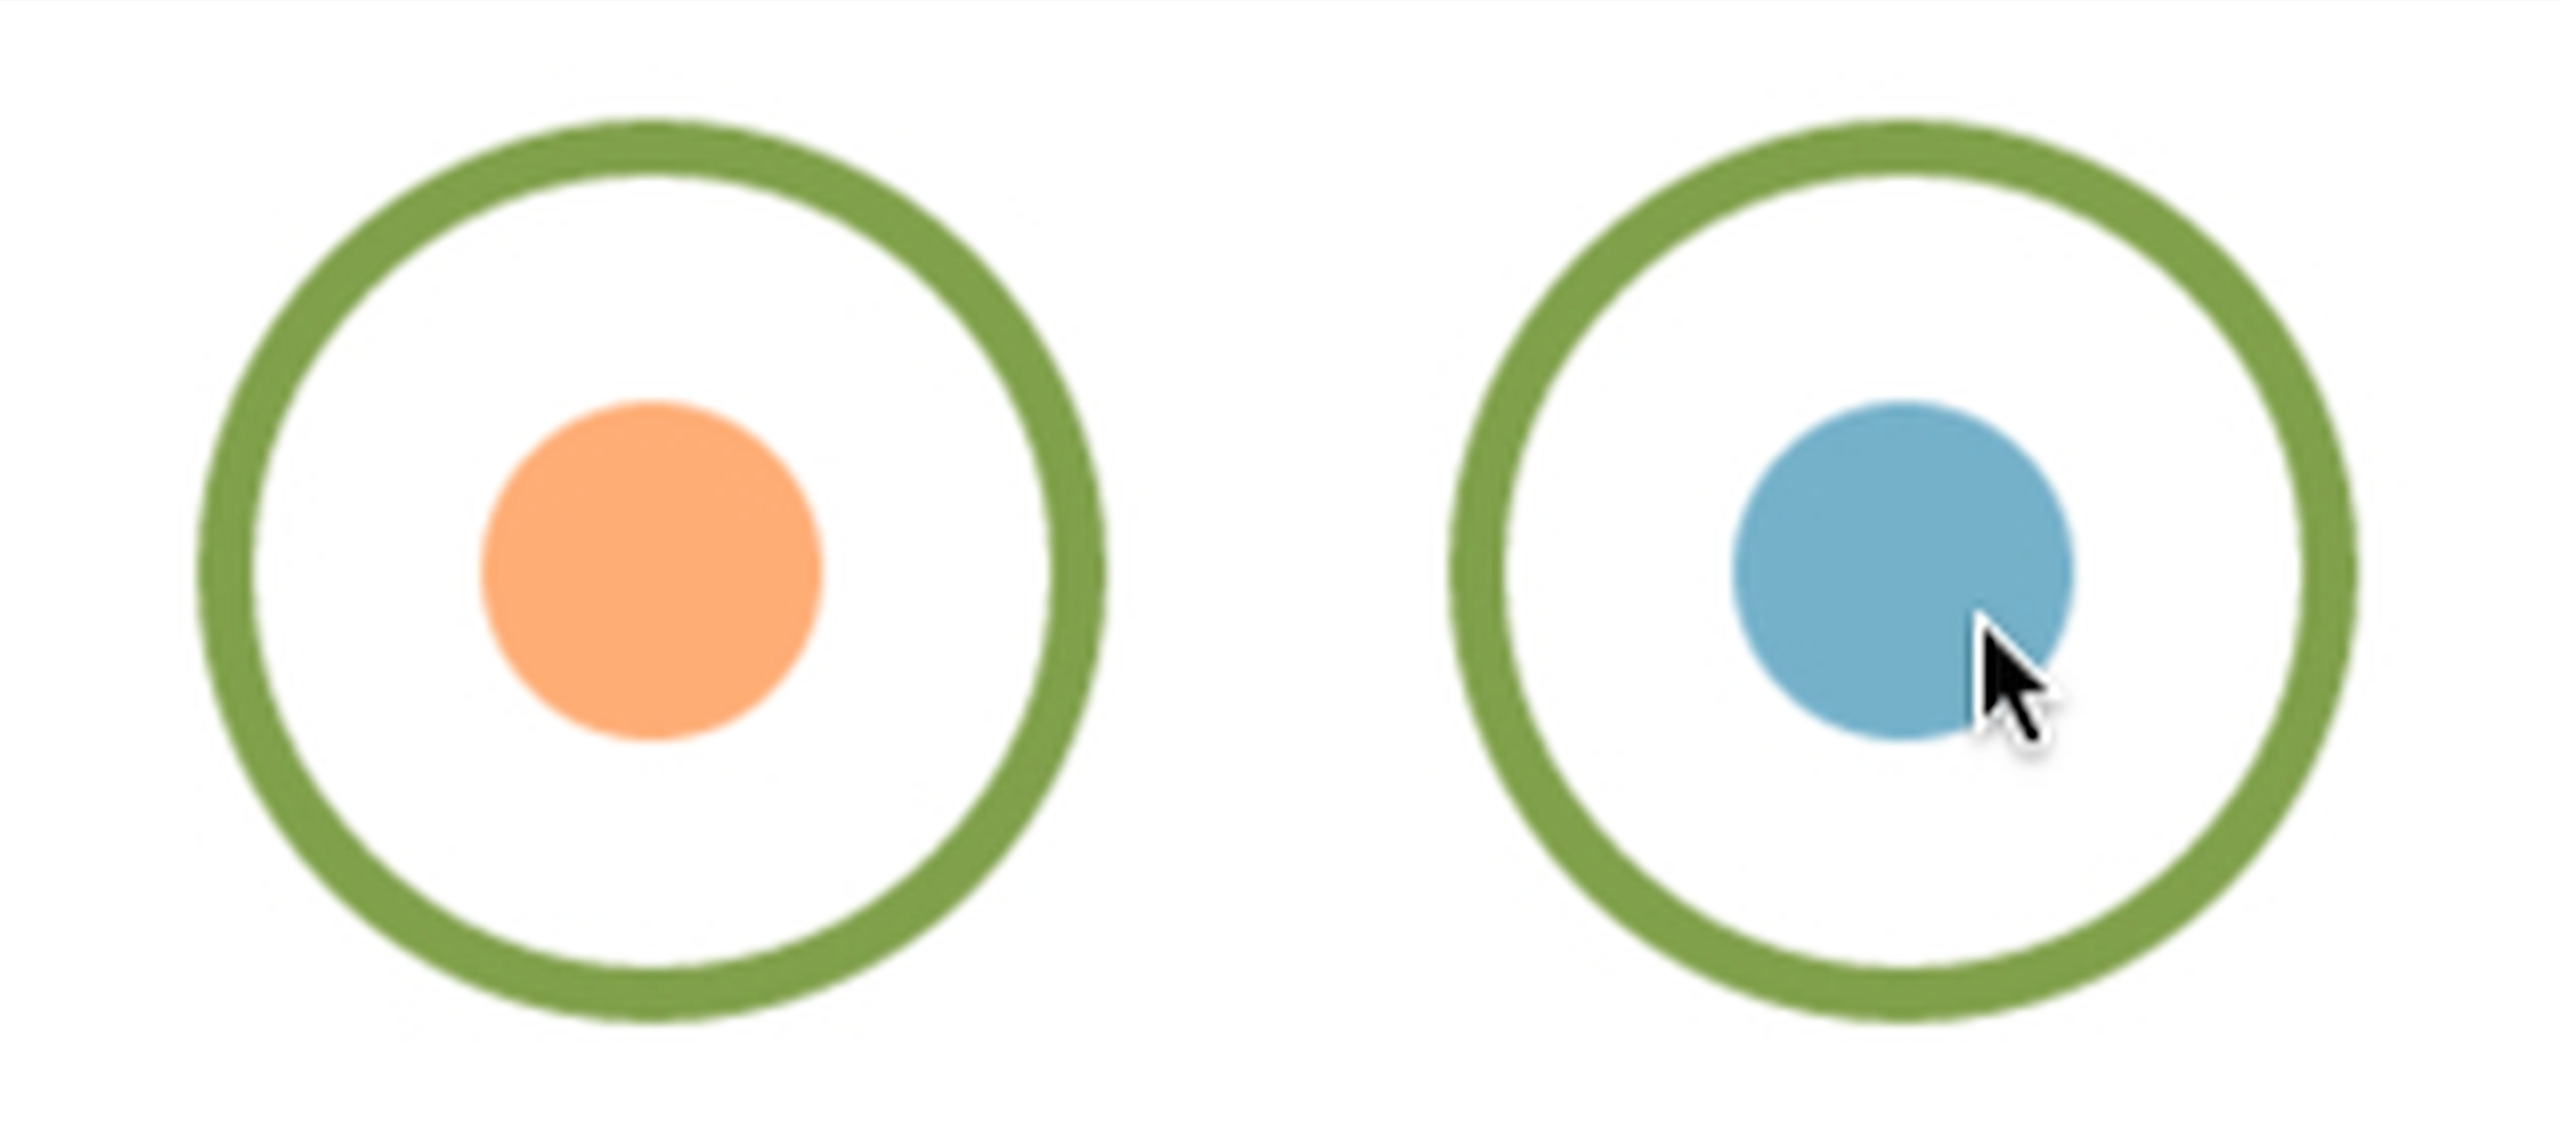
\includegraphics[width=0.6\textwidth]{joysticks}
\caption{Joysticks.}
\label{fig:joysticks}
\end{figure}


Para dotar a éste círculo de movimiento hemos utilizado los eventos de JavaScript \emph{mousedown}, \emph{mousemove}, \emph{mouseup} y \emph{mouseout}. El primer evento se ejecuta cuando el usuario hace \emph{click} con el ratón. Dentro de este evento nos encargamos de detectar si ese \emph{click} ha sido en el círculo que hemos dibujado. El segundo evento ocurre cuando, sin soltar el ratón, el usuario lo mueve. Si en el primer evento hemos detectado que ha \emph{clickado} sobre el círculo, se re-dibuja por la zona donde está moviendo el ratón. Con el evento \emph{mouseup}, al deshacer el click, re-dibujamos el círculo a su posición inicial. El evento \emph{mouseout} detecta si el ratón se ha salido del aro y también devuelve el \emph{joystick} a su posición inicial.\\

\begin{lstlisting}[caption=Movimiento y control del joystick.]
canvas.addEventListener('mousedown', function(evt) {
        var mousePos = oMousePos(canvas, evt);

        if (ctx.isPointInPath(mousePos.x, mousePos.y)) {
                arrastrar = true;
       }
}, false);

// mousemove 
canvas.addEventListener('mousemove', function(evt) {
        var m = oMousePos(canvas, evt);
        //ctx.beginPath();
        //ctx.arc(X, Y, maxR, 0, 2 * Math.PI);
        if (arrastrar) {
                delta.x = m.x - p.X;
                delta.y = m.y - p.Y;
                var deltaR = Math.sqrt(delta.x * delta.x + delta.y * delta.y);
                var elR = Math.min(deltaR, maxR);
                //console.log("DeltaR: " + deltaR + " elR: " + elR);
                var angulo = Math.atan2(delta.y, delta.x);
                //console.log(angulo); //
                
                x = X + elR * Math.cos(angulo);
                y = Y + elR * Math.sin(angulo);
                
                ctx.clearRect(0, 0, cw, ch); // Clear and redraw the joystick
                dibujarAro(X, Y, RHoop);
                dibujarCirculo(x, y, RCircle);
        }
}, false);

// mouseup 
canvas.addEventListener('mouseup', function() {
        
        sendAltYaw(0, 0);
        
        arrastrar = false;
        ctx.clearRect(0, 0, cw, ch);
        dibujarAro(X, Y, RHoop);
        dibujarCirculo(X, Y, RCircle);
}, false);

// mouseout 
canvas.addEventListener('mouseout', function() {
        sendAltYaw(0, 0);
        
        arrastrar = false;
        ctx.clearRect(0, 0, cw, ch);
        dibujarAro(X, Y, RHoop);
        dibujarCirculo(X, Y, RCircle);
}, false);
\end{lstlisting}

Dentro del evento \emph{mousemove} también recogemos la posición en la que se encuentra el \emph{joystick} y llamamos a la función correspondiente que se ocupa de enviar los datos a través del canal RTCDataChannel. En el \emph{joystick} izquierdo se llama a la función \emph{sendCMDVel()} y en el de la derecha a \emph{sendAltYaw()}.\\

Para dotar a los joysticks de funcionalidades táctiles hemos desarrollado las mismas funciones que las anteriores con los eventos táctiles equivalentes: \emph{touchstart}, \emph{touchmove}, \emph{touchend}, \emph{touchup}.\\

Estos joysticks se han situado en las esquinas inferiores de la pantalla como se puede observar en la figura \ref{fig:interfazweb} para facilitar el manejo con dispositivos táctiles.\\

\subsubsection{Gamepad}

También se ha desarrollado la posibilidad de teleoperar el drone mediante un mando USB conectado al ordenador. La API \emph{Gamepad} de JavaScript no está estabilizada, hay navegadores que no la soportan y no todos los mandos funcionan de la misma manera. El mando con el que se ha desarrollado es el \emph{Xbox} de la empresa \emph{Microsoft}, no se han realizado pruebas con mandos de otros fabricantes por lo que no se puede asegurar su correcto funcionamiento. \\

Para la detección del mando al ser conectado al puerto USB hemos usado los eventos que nos da la API \emph{Gamepad}. Al conectar el mando se ejecuta el evento \emph{gamepadconnected} que llama a la función manejadora \emph{connecthandler}.\\

\begin{lstlisting}[caption=Detección del mando.]
function connecthandler() {
    var gp = navigator.getGamepads()[0];
    console.log("Gamepad connected at index %d: %s. %d buttons, %d axes.", gp.index, gp.id, gp.buttons.length, gp.axes.length);
    updateGPInterval = setInterval(updateGamePad, 100);
    $(".joystick").fadeOut(4000);
}

window.addEventListener("gamepadconnected", connecthandler);
window.addEventListener("gamepaddisconnected", disconnecthandler);
\end{lstlisting}

La función \emph{connecthandler()} guarda en una variable el mando conectado y crea un intervalo que llama periódicamente a la función que detectará los movimientos de los botones. Por otro lado se encarga de ocultar los \emph{joysticks} virtuales, los cuales volveremos a mostrar si se desconecta el mando.\\

Dentro de la función \emph{updateGamePad()} detectamos el movimiento de los dos \emph{joysticks} del mando. y la pulsación de los botones. Hemos configurado la pulsación de una tecla para el despegue y otra para el aterrizaje, y con los \emph{joysticks} controlamos el vuelo de igual manera que con los \emph{joysticks} virtuales.\\

\begin{lstlisting}[caption=Manajador de mando.]
function updateGamePad() {
    var gp = navigator.getGamepads()[0];
    if (!gp && isChrome) {
        disconnecthandler();
        chromeInterval = setInterval(scangamepad, 1000);        
    } else {
        if (gp.buttons[0].pressed) {
            enviarOrden("takeoff");
        } else if (gp.buttons[1].pressed) {
            enviarOrden("land");
        }
        
        if (!isChrome) {
            var Y = applyDeadzone(gp.axes[0], 0.12);
            var X = applyDeadzone(gp.axes[1], 0.12);
            var Yaw = applyDeadzone(gp.axes[3], 0.12);
            var Alt = applyDeadzone(gp.axes[4], 0.12);
        } else{
            var Y = applyDeadzone(gp.axes[0], 0.12);
            var X = applyDeadzone(gp.axes[1], 0.12);
            var Yaw = applyDeadzone(gp.axes[2], 0.12);
            var Alt = applyDeadzone(gp.axes[3], 0.12);
         }
         sendCMDVel(-X*velocidad,Y*velocidad);// Change variables and send the command to the drone
         sendAltYaw(-Alt*velocidad, Yaw*velocidad);
    }
}
\end{lstlisting}

En esta función también recogemos los valores y llamamos a las funciones encargadas de enviar los datos a través del canal \emph{RTCDataChannel}.\\


\subsection{Relojes de navegación}\label{subsec:relojesnavegacion}

Para representar los datos recibidos de los sensores del drone como la altitud, velocidad, brujula, etc nos hemos ayudado de un plugin\footnote{http://sebmatton.github.io/flightindicators/}\cite{jqueryflightindicator} jQuery desarrollado por Matton Sébastien\footnote{https://github.com/sebmatton}.\\

Hemos usado cuatro relojes distintos: 

\begin{itemize}
\item Uno que nos indique la altitud del drone.
\item El segundo nos representa el horizonte.
\item El tercero es una brújula.
\item El cuarto indica la inclinación del drone.
\end{itemize}

Para crear estos relojes, creamos una etiqueta \texttt{<span>} de HTML5 para cada reloj, y posteriormente con jQuery llamamos a las siguientes funciones:\\

\begin{lstlisting}[caption=Creación de los relojes.]
var attitude = $.flightIndicator('#attitude', 'attitude', {roll:50, pitch:-20, size:s, showBox : false}); // Horizon
var heading = $.flightIndicator('#heading', 'heading', {heading:150, showBox:false, size:s}); // Compass
var altimeter = $.flightIndicator('#altimeter', 'altimeter', { showBox:false, size:s});
var turn_coordinator = $.flightIndicator('#turn_coordinator', 'turn_coordinator', {turn:0,  showBox:false, size:s}); 
\end{lstlisting}

Para actualizar los datos de estos relojes con los que llegan al par remoto directamente desde el drone se ha desarrollado una función a la que llamamos periódicamente con las variables \emph{pose} y \emph{navdata} como argumentos:\\

\begin{lstlisting}[caption=Actualización de los relojes.]
this.updatePanelControl =  function(navdata, pose){
    // calculate yaw, pitch, and roll
    var yaw = getYaw(pose.q0, pose.q1, pose.q2, pose.q3);
    var pitch = getPitch(pose.q0, pose.q1, pose.q2, pose.q3);
    var roll = getRoll(pose.q0, pose.q1, pose.q2, pose.q3);
    
    attitude.setRoll(roll);
    attitude.setPitch(-pitch);

    // Altimeter update
    altimeter.setAltitude(pose.z*100);
    //altimeter.setPressure(1000+3*Math.sin(increment/50));

    // TC update
    turn_coordinator.setTurn(roll);

    // Heading update
    heading.setHeading(yaw);
    
    // Cambiamos el ancho en el estilo del relleno de la bateria segun el nivel de bateria que nos manda el drone
    battery.style.width = String(navdata.batteryPercent) + "%";
    window.navdata = navdata;
    console.log(navdata.state);
}
\end{lstlisting}

La situación en la pantalla de estos relojes es de gran importancia. Para no ocultar la visión de la cámara y tenerlos visibles se ha decido colocarlos por pares en las esquinas superiores de la pantalla. Además, se les ha dotado de la propiedad \emph{draggable} de jQuery la cuál nos permite arrastrarlos por la pantalla y situarlos dónde más cómodo le sea al usuario.\\

\begin{lstlisting}[caption=Elementos arrastrables.]
$(function() {
    $( "#attitude").draggable();
    $( "#altimeter").draggable();
    $( "#turn_coordinator").draggable();
    $( "#heading").draggable();
});
\end{lstlisting}

En la figura \ref{fig:relojesnavegacion} podemos observar los cuatro relojes incorporados a la interfaz web de usuario. En la figura \ref{fig:interfazweb} se pueden también observar integrados con el resto de elementos que componen la interfaz.\\

\begin{figure}[h!]
\centering
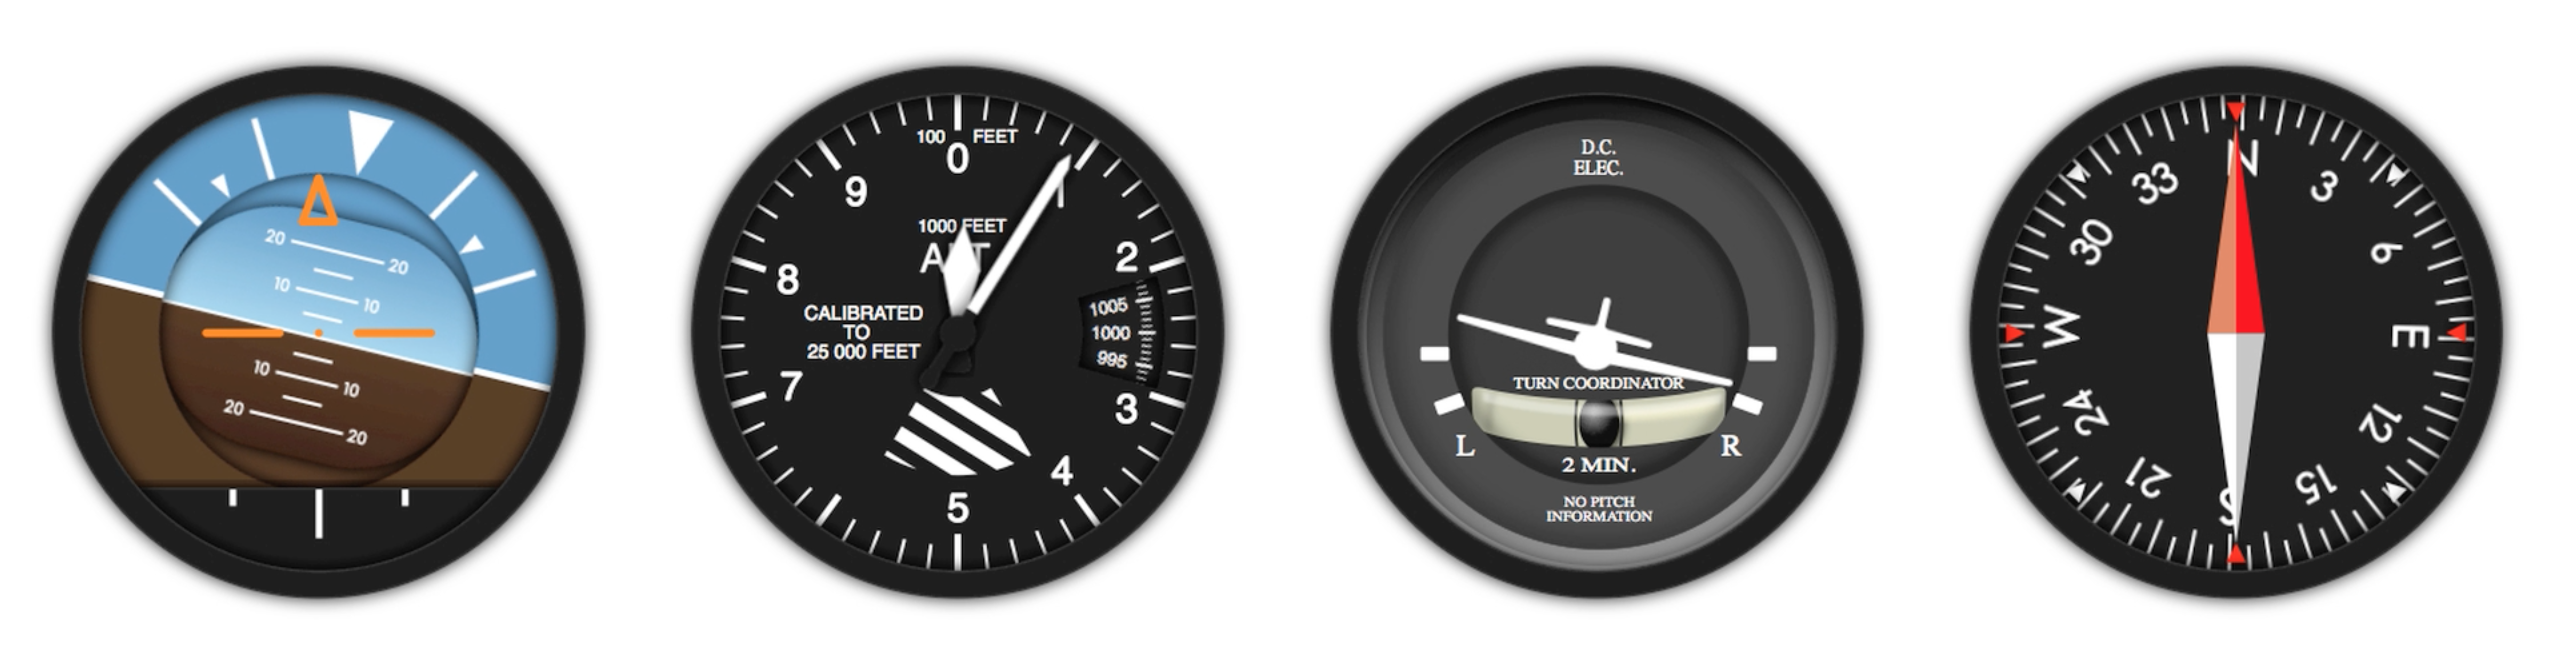
\includegraphics[width=0.9\textwidth]{relojesnavegacion}
\caption{Relojes de navegación.}
\label{fig:relojesnavegacion}
\end{figure}

\subsection{Visualización espacial 3D del drone}

Para días de niebla o condiciones extremas es imprescindible tener localizada la posición del drone para poder traerlo de vuelta. Utilizando los datos del GPS del drone hemos creado un marco 3D con la situación del drone en tiempo real. Para desarrollar este visualizador 3D nos hemos ayudado de la librería \emph{Three.js}\footnote{http://threejs.org} la cuál nos facilita el acceso y uso de WebGL. El mapa 3D es dibujado sobre una etiqueta \texttt{<canvas>}, y está compuesto principalmente por una escena, una cámara de observación en esa escena (desde ella se ve la escena), el suelo y el drone.\\

Lo primero que hemos hecho ha sido crear la escena y situar la cámara en la misma.\\

\begin{lstlisting}[caption=Escena y cámara en el mapa 3D.]
// Escena
var scene = new THREE.Scene();

//Camara
var camera = new THREE.PerspectiveCamera( 45, mapa.width/mapa.height, 0.1, 1000 );
camera.up.set( 0, 0, 1 );
camera.position.set( 18,20, 18 );
camera.lookAt( new THREE.Vector3( 0, 0, 0 )  );
\end{lstlisting}

La cámara se ha decidido que esté fija apuntando a la posición inicial del drone, ya que de esta manera es más sencillo conocer la posición del drone y devolverlo al origen si fuese necesario.\\

Posteriormente añadimos la superficie que representa el suelo con una rejilla de celdas de 1m$^{2}$.\\

\begin{lstlisting}[caption=Superficie que representa el suelo del mapa.]
// Suelo. 
var planeGeometry = new THREE.PlaneGeometry( 40, 40);
var planeMaterial = new THREE.MeshLambertMaterial( {color: 0xcccccc} );
var plane = new THREE.Mesh( planeGeometry, planeMaterial );
plane.position.x = 0;
plane.position.y = 0;
plane.position.z = 0;
plane.castShadow = false;
plane.receiveShadow = true;
scene.add( plane );
\end{lstlisting}

Three.js admite archivos en formato COLLADA \emph{(COLLAborative Design Activity)}. Hemos reutilizado los archivos Collada que utiliza el simulador Gazebo para representar de igual manera el drone. Cargamos el objeto collada del cuadricóptero, establecemos su posición inicial en el mapa y su tamaño de la siguiente manera:\\

\begin{lstlisting}[caption=Carga del objeto collada.]
var loader = new THREE.ColladaLoader();

loader.load('./collada/quadrotor/quadrotor_4.dae', function ( collada ) {
  
  dae = collada.scene;
  
  dae.position.x = 0;
  dae.position.y = 0;
  dae.position.z = 1;
  dae.scale.x = dae.scale.y = dae.scale.z = 5;
  dae.updateMatrix();
   
  daemesh = dae.children[0].children[0];
  daemesh.castShadow = true;
  daemesh.receiveShadow = true;
      
  scene.add( dae );
  render();
});
\end{lstlisting}

Desde aquí se hace también la primera llamada a la función \emph{render()} que se encargara de actualizar la posición del drone en el mapa. Este re-pintado se produce con la función \emph{requestAnimationFrame()}, la cuál admite como argumento la función a actualizar.\\

\begin{lstlisting}[caption=Actualización del lienzo.]
var render = function () {
  if (pose == undefined) {
    dae.position.x = 0;
    dae.position.y = 0
    dae.position.z = 0;
  }else {
    dae.quaternion.set(pose.q1, pose.q2, pose.q3, pose.q0);
    dae.position.set(pose.x, pose.y, pose.z);
      
    panelControl.updatePanelControl(navdata, pose);// update sensors watchers
  }

  renderer.render(scene, camera);
  requestAnimationFrame( render );
};
\end{lstlisting}

Para liberar al navegador de un \emph{setInterval()}, se aprovecha el 'intervalo' que crea \emph{requestAnimationFrame()} lo utilizándolo para llamar a la función \emph{updatePanelControl()} que actualiza los relojes de navegación. En la figura \ref{fig:mapa3d} se puede ver el resultado final del mapa.\\

\begin{figure}[h!]
\centering
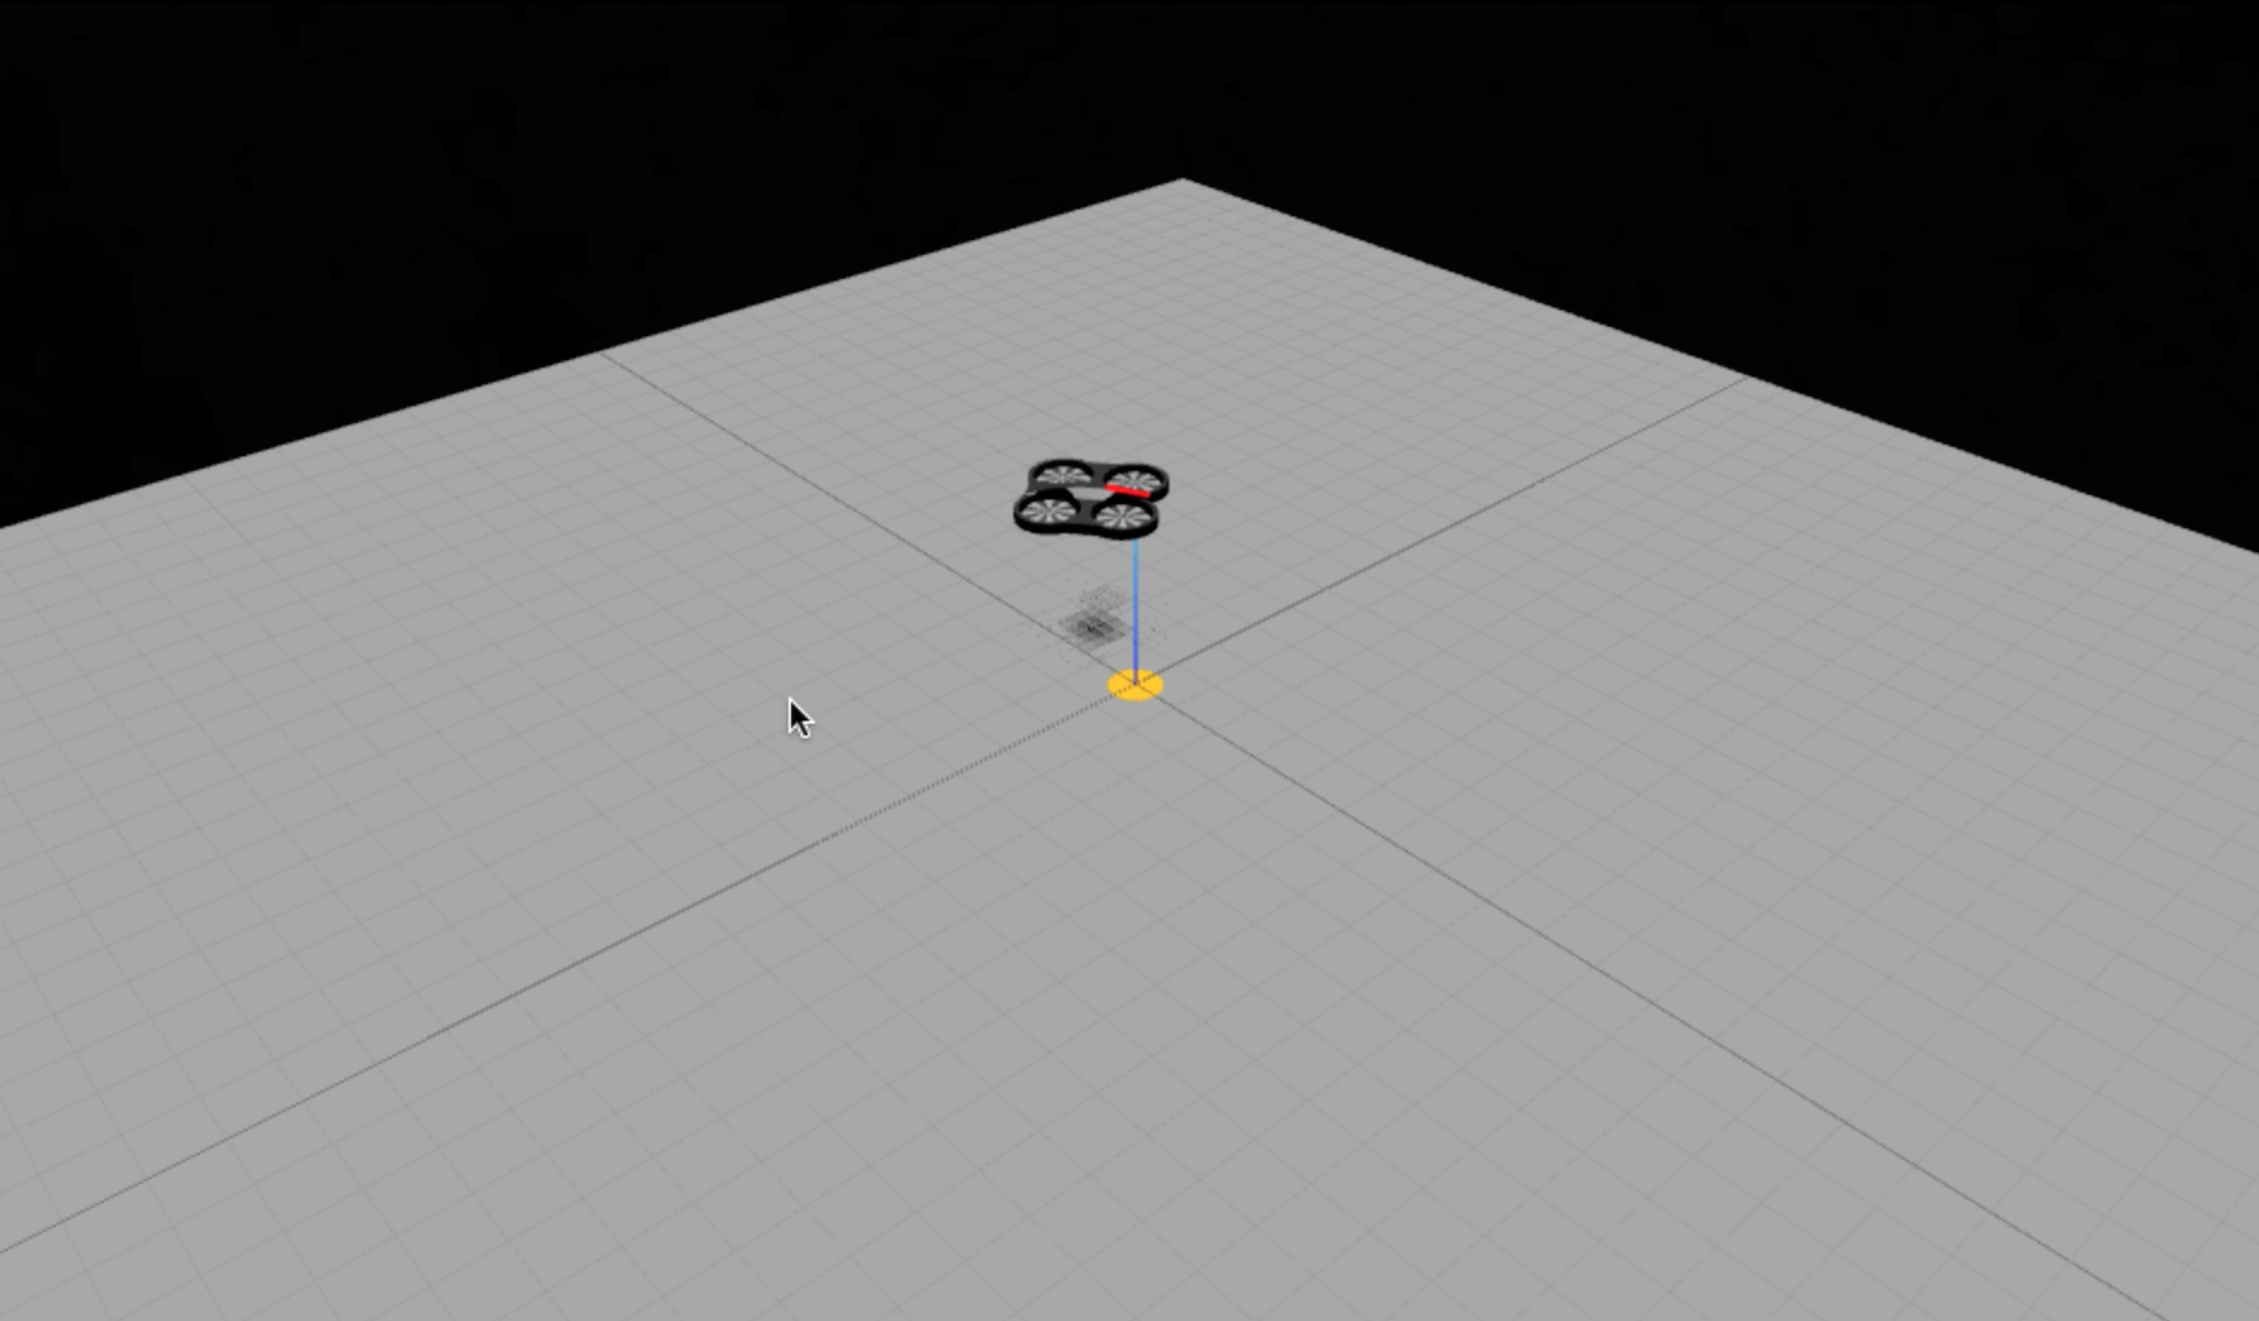
\includegraphics[width=0.6\textwidth]{mapa3d}
\caption{Mapa 3D con three.js}
\label{fig:mapa3d}
\end{figure}


Además se le han añadido dos funcionalidades más a la interfaz web. Por un lado se ha añadido un indicador de nivel de batería, creado en HTML5 y CSS3. Esta batería está desarrollada por Jon Kantner\footnote{http://codepen.io/jkantner/}\cite{bateria} y la hemos adaptado para nuestro proyecto. Por otro lado, se ha añadido un control de velocidad del drone, para facilitar su manejo si las condiciones son extremas o si se está realizando un vuelo en interiores. Este control está también desarrollado con HTML5 y CSS3 y fijan la velocidad máxima ordenable con los \emph{joysticks} visuales y el mando. Estos dos elementos están situados en la parte central superior de la pantalla como se puede ver en la figura \ref{fig:bateriayvelocidad}.\\

\begin{figure}[h!]
\centering
  \begin{subfigure}[]{60mm}
    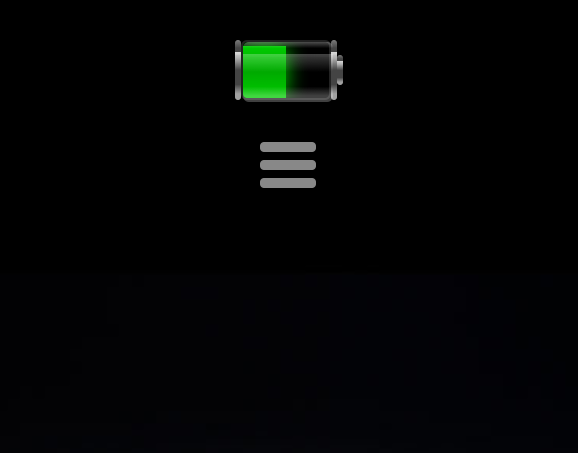
\includegraphics[width=60mm]{extras1}
    \caption{Control de velocidad sin desplegar.} 
  \end{subfigure}
  \hspace{5pt}
  \begin{subfigure}[]{60mm}
    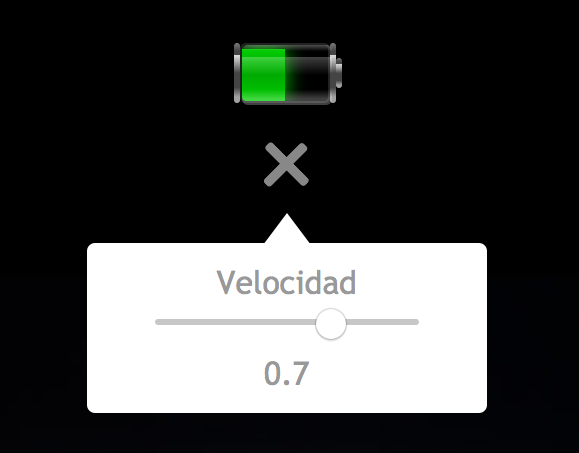
\includegraphics[width=60mm]{extras2}
    \caption{Control de velocidad desplegado.}
  \end{subfigure}
  \caption{Control de bateria y velocidad del cuadricoptero.}\label{fig:bateriayvelocidad}
\end{figure}


El resultado final de la interfaz web de usuario con todos los elementos integrados se puede ver en la figura \ref{fig:interfazweb}.


\begin{figure}[h!]
\centering
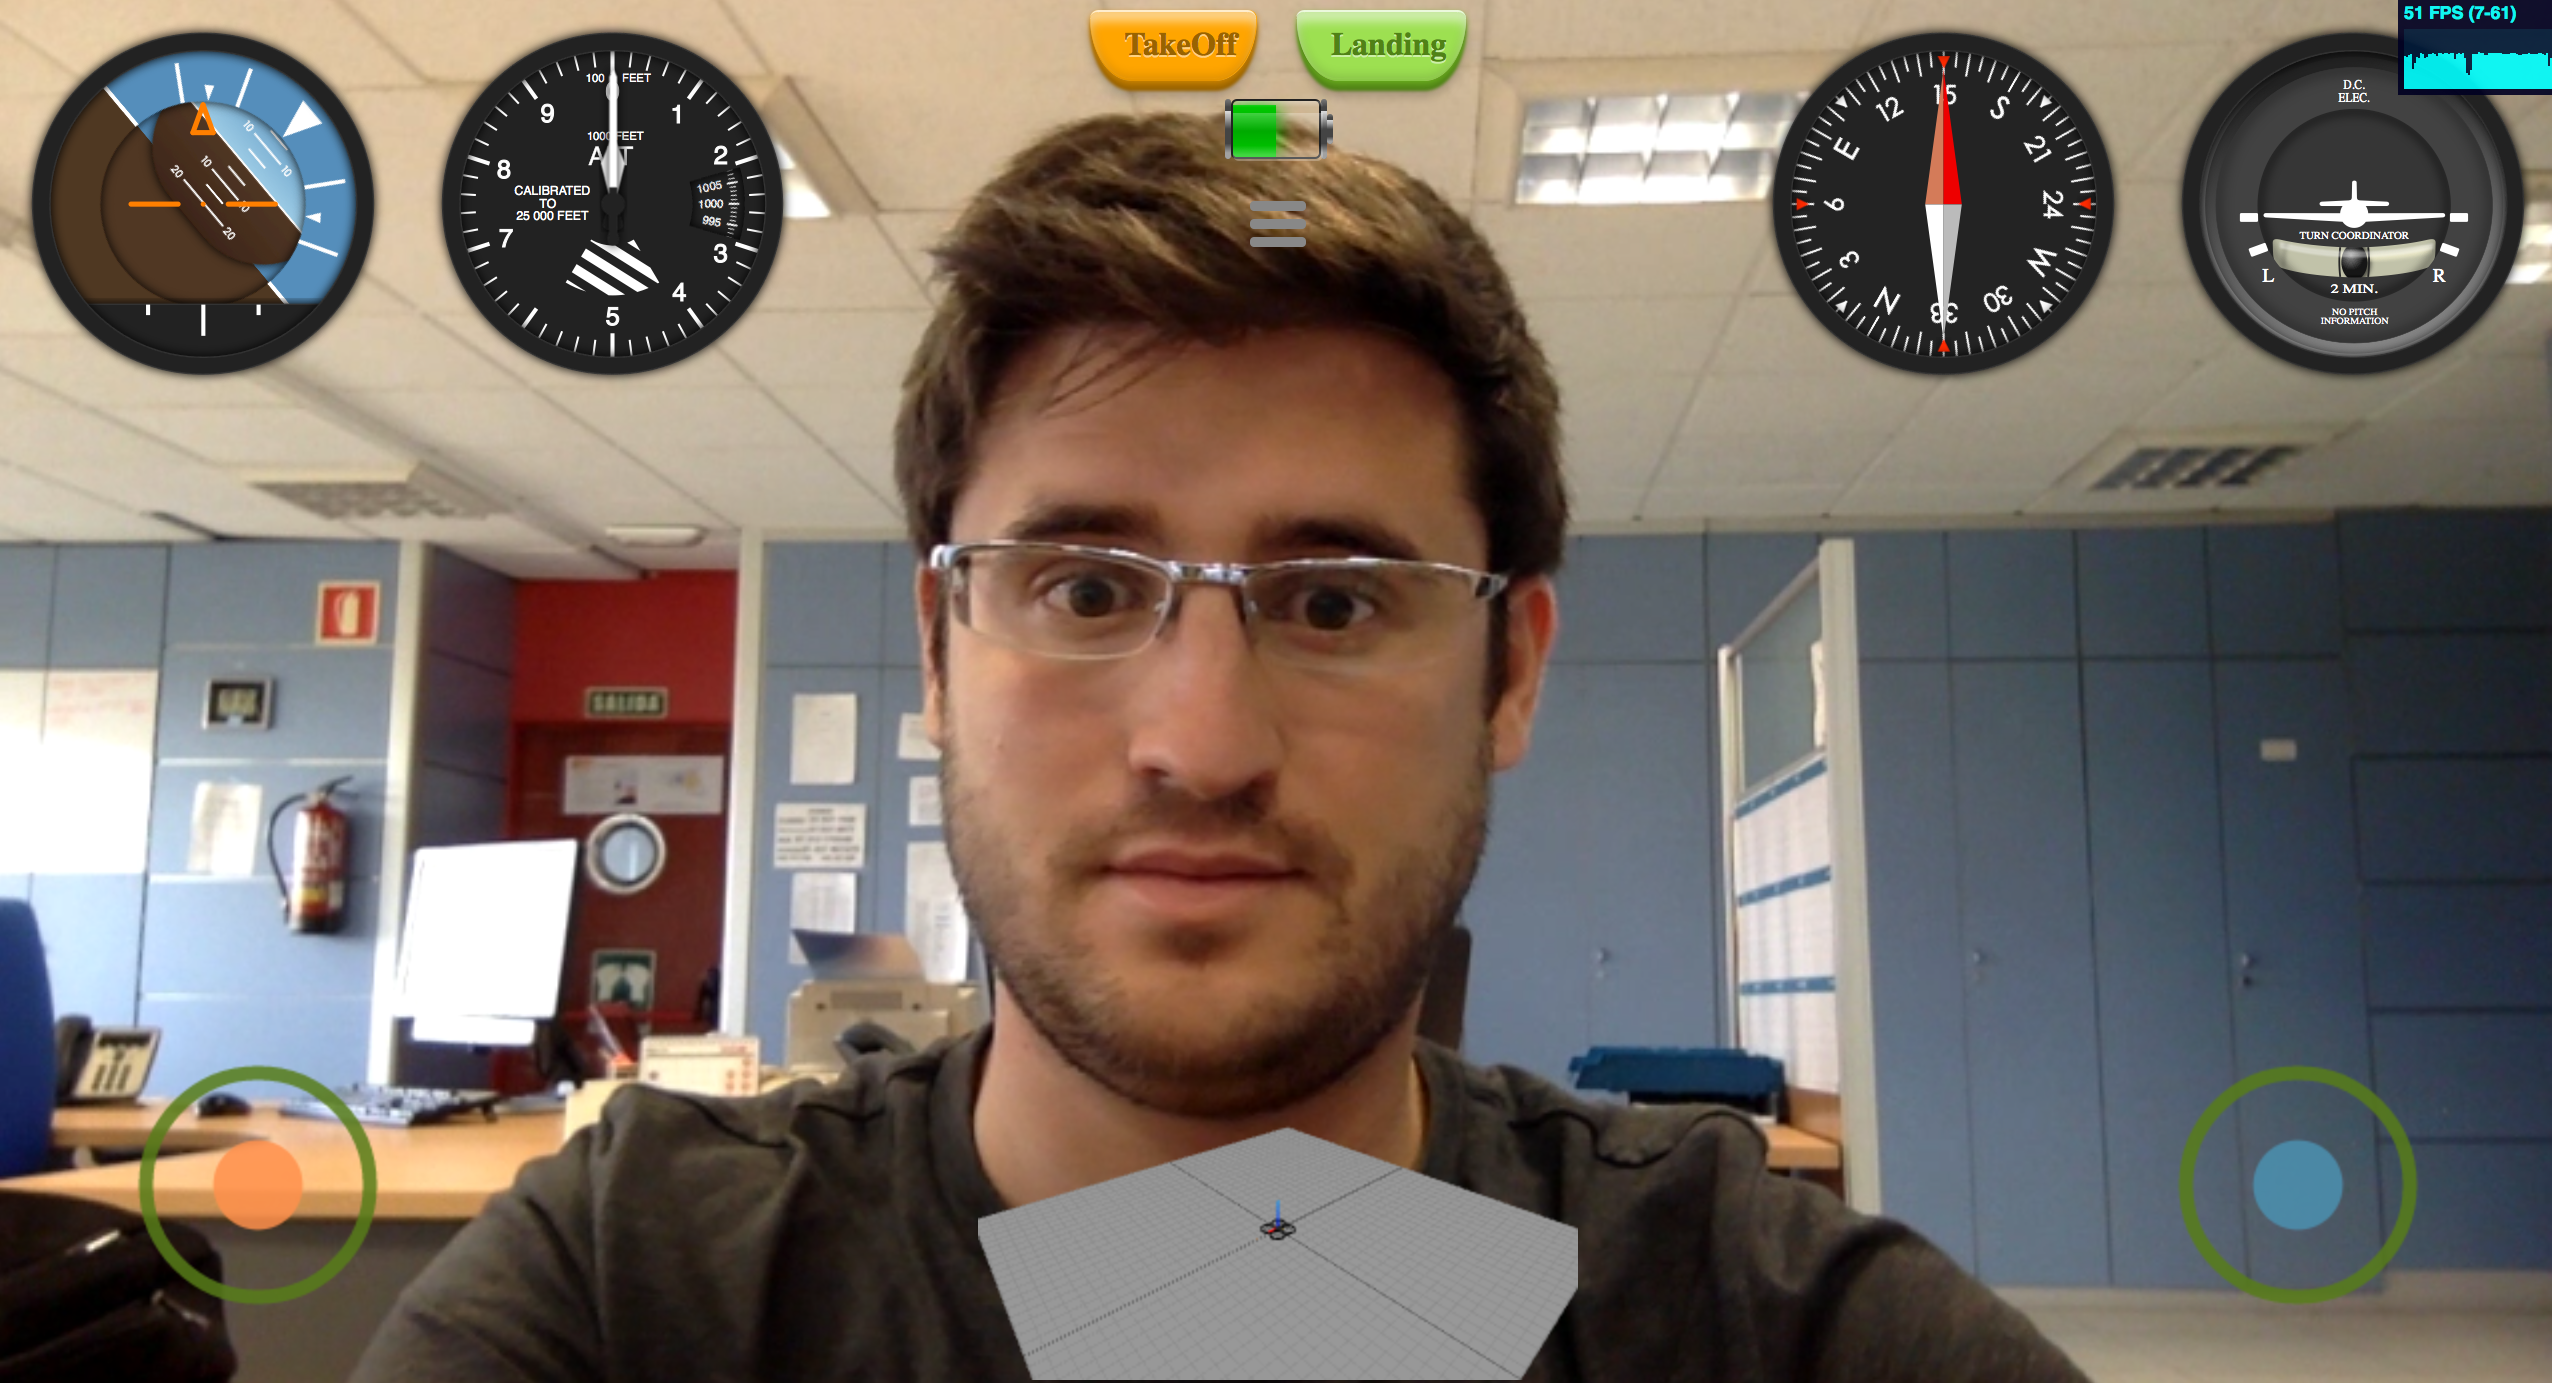
\includegraphics[width=0.9\textwidth]{interfazweb}
\caption{Interfaz web de usuario.}
\label{fig:interfazweb}
\end{figure}

\chapter{Experimentos}

En capítulos anteriores se han expuesto los objetivos marcados para la realización del proyecto así como la solución desarrollada para cada uno de estos problemas y las herramientas utilizadas para las mismas. En este capítulo se muestran los experimentos que se han ido realizando según íbamos cumpliendo objetivos.\\

\section{Simulador Gazebo}

Una vez desarrollado el proyecto y satisfaciendo todos los objetivos marcados se han realizado pruebas sobre la plataforma de simulación Gazebo para comprobar sin ningún tipo de riesgos el funcionamiento del mismo.\\

Para realizar este experimento asemejandose de la manera más realista al experimento final con el drone real se ha utilizado un \emph{Intel Compute Stick}\footnote{\url{http://www.intel.com/content/www/us/en/compute-stick/compute-stick-product-brief.html}} como par local, encargado de conectarse a las interfaces ICE que nos proporciona el plugin ArDrone desarrollado por JdeRobot para el simulador Gazebo. Este ordenador está compuesto por un procesador Intel Atom que corre Ubuntu 14.04 LTS como sistema operativo. El simulador Gazebo se ha ejecutado en el mismo equipo que correrá el navegador remoto, desde el que teledirigimos el drone.\\

Los resultados de este experimento han sido muy positivos, el control y manejo del drone ha sido de manera fluida y sin realizar ningún tipo de movimiento extraño producido por algún tipo de mal-funcionamiento del código. El manejo se ha realizado tanto con los \emph{joysticks} virtuales como con el mando.\\

Una vez superado este experimento se ha realizado el siguiente, consistiendo en realizar pruebas con el drone real.\\

\section{Vuelo del drone real}

Las pruebas con el drone real se han divido a su vez en dos. La primera consiste en realizar las pruebas sin colocar a bordo del drone ni el \emph{computer stick} ni la cámara. Ambos se han usado para las pruebas pero para una primera aproximación se han realizado sin estar a bordo.\\

Así pues la distribución de los equipos es: computer stick como par local, que se conecta al drone real y accede a la cámara USB conectada al mismo, y ordenador portátil como par remoto desde el que se teleoperará el drone y a su vez está ejecutando el servidor de señalización y el \texttt{ardrone\_server.} La figura \ref{fig:experimentodronereal1} muestra la realización de este experimento. En la mediawiki\footnote{\url{http://jderobot.org/Irodmar-tfg\#First\_Flying\_with\_Real\_Drone}}\cite{Mediawiki} hay un vídeo completo del mismo.\\

\begin{figure}[h!]
\centering
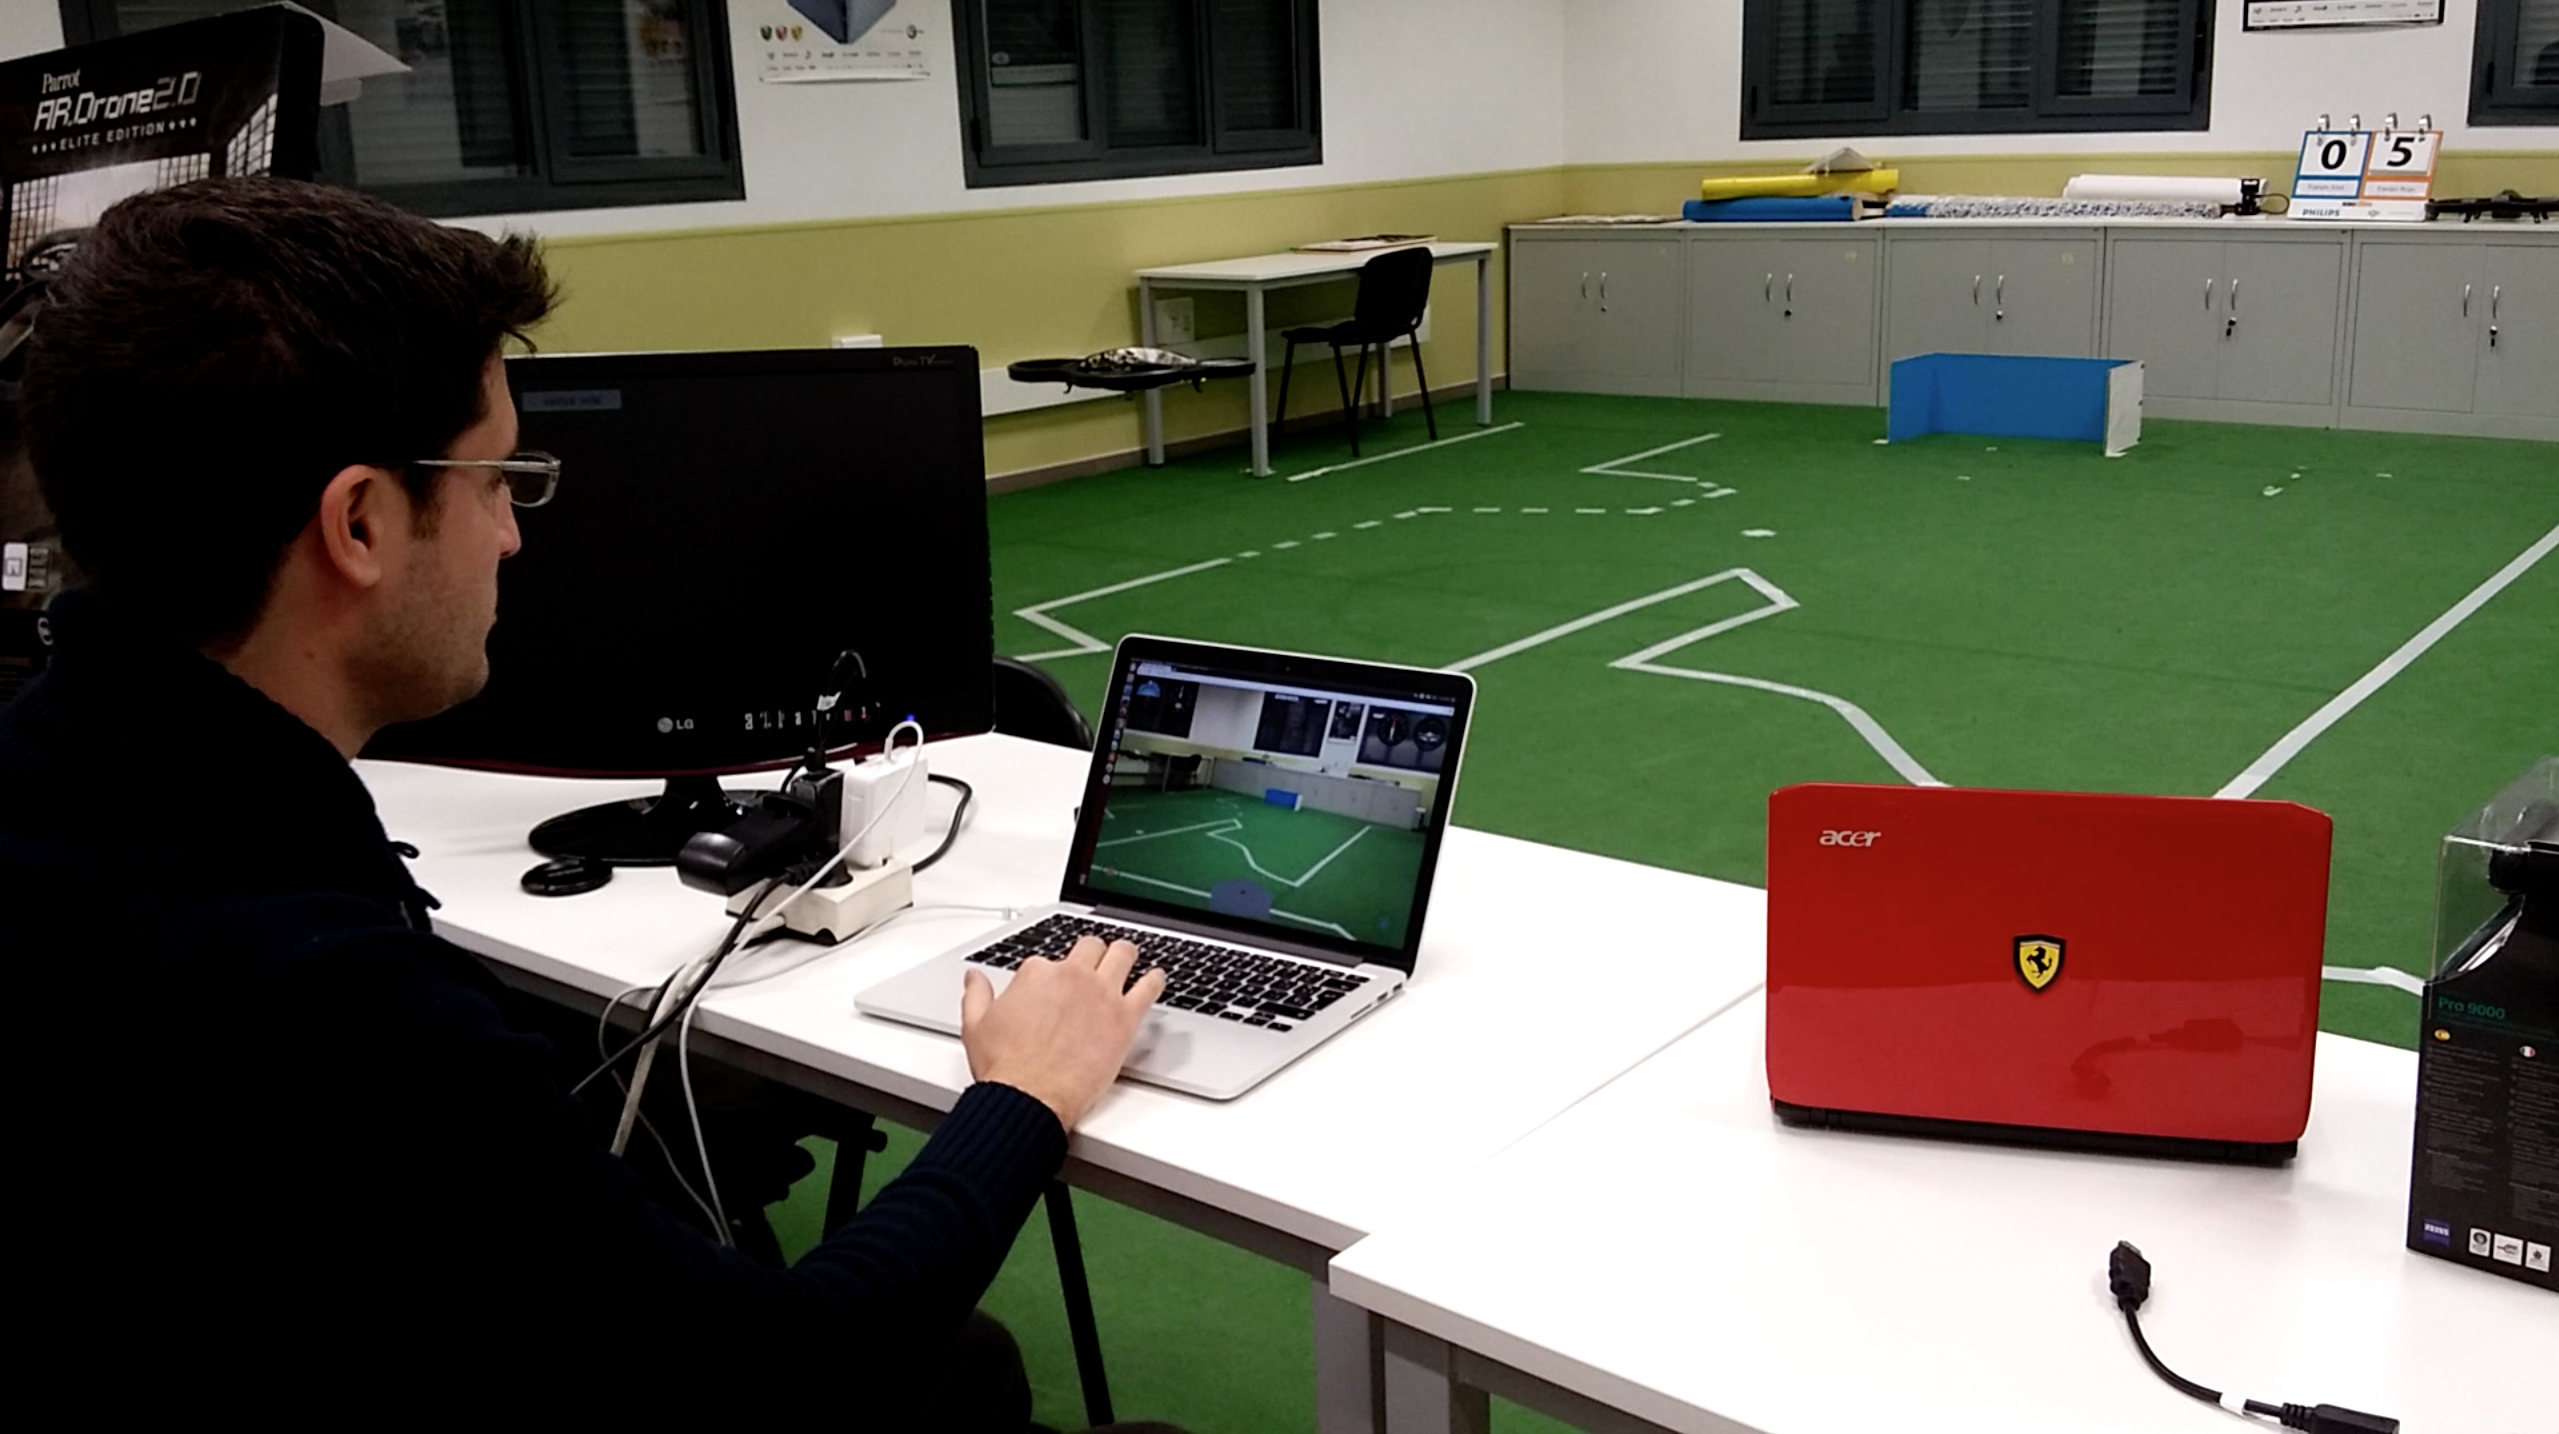
\includegraphics[width=0.9\textwidth]{experimentodronereal1}
\caption{Experimento uno con drone real.}
\label{fig:experimentodronereal1}
\end{figure}

Esta prueba también ha sido un éxito, por lo que nos marcamos el siguiente experimento con el drone y la cámara a bordo del drone. Este experimento la configuración es la misma que en el anterior, pero el manejo del drone con la aplicación será más realista ya que tenemos la cámara en primera persona.\\

*** FIN EXPERIMENTO CON FOTO Y LINK AL VIDEO***


\section{Vuelos con multidispositivos}

Como tercer y último experimento hemos probado a volar el drone utilizando dispositivos móviles. WebRTC tiene soporte para dispositivos móviles y los elementos de control los hemos desarrollado también para dispositivos táctiles, podemos utilizarlos como par remoto, par local o ambos. Al igual que el experimento anterior se ha realizado en dos pasos, primero sin colocar el dispositivo a bordo del drone para confirmar su correcto funcionamiento y posteriormente repitiéndolo con el dispositivo a bordo. Realizar experimentos con dispositivos móviles implica la necesidad de la utilización de un ordenador de apoyo que será el que ejecute tanto el servidor de señalización para WebRTC cómo \emph{ardrone\_server}.\\

Como primer experimento se ha utilizado un ordenador como par local y un móvil como par remoto desde el que gobernamos los movimientos del drone. En la figura \ref{fig:experimentodronemultidispositivo1} se puede apreciar un momento del vídeo del experimento\footnote{\url{http://jderobot.org/Irodmar-tfg\#Flying\_with\_a\_mobile\_like\_Remote\_PC}}.\\

\begin{figure}[h!]
\centering
\includegraphics[width=0.9\textwidth]{experimentodronemultidispositivo1}
\caption{Experimento con móvil como par remoto.}
\label{fig:experimentodronemultidispositivo1}
\end{figure}

El segundo experimento es a la inversa, se utiliza un ordenador como par remoto y un dispositivo móvil como par local, encargándose de establecer la conexion con el drone. En este caso las imágenes que se envían son las de cualquieras de las dos cámaras del móvil, la delantera o la trasera. La figura \ref{fig:experimentodronemultidispositivo2} muestra un momento del experimento que esta recogido en un vídeo en la mediawiki\footnote{\url{http://jderobot.org/Irodmar-tfg#Flying_with_a_mobile_like_Droner_PC}}.\\

\begin{figure}[h!]
\centering
\includegraphics[width=0.9\textwidth]{experimentodronemultidispositivo2}
\caption{Experimento con móvil como par local.}
\label{fig:experimentodronemultidispositivo2}
\end{figure}
\chapter{Conclusiones y trabajos futuros}

En capítulos anteriores hemos descrito el contexto y el problema que abordamos en este proyecto, los objetivos iniciales y la solución propuesta junto con una serie de pruebas y experimentos que validad y caracterizan el proyecto. En este capítulo se exponen las conclusiones obtenidas y las posibles líneas por las que se puede continuar el trabajo.\\

\section{Conclusiones}

Bajo una mirada retrospectiva se puede observar que se han cumplido los objetivos generales que nos habíamos marcado. Hemos creado una aplicación web entre navegadores sin servidores intermedios que nos permite controlar, manejar y monitorizar un cuadricóptero. Dentro de este objetivo nos marcamos tres subjetivos, los cuáles también hemos cumplido:\\

\begin{itemize}
\item Hemos creado una conexion local directamente con los sensores y actuadores del drone mediante un navegador web sin necesidad de servidores intermedios.
\item Se ha desarrollado una conexión entre navegadores que transfieren en tiempo real y sin servidores intermedios la cámara y los datos necesarios para monitorar los sensores del drone y teleoperarlo.
\item Se ha creado una interfaz web amigable que nos permite monitorar la cámara y los sensores del drone, así como teleoperarlo de una manera muy intuitiva y sencilla de usar.
\item A parte de estos subobjetivos se le han añadido unos extras, como poder teleoperarlo con un mando o que tanto la conexión local como remota, así como la interfaz sean multiplataforma y multidispositivo, lo que nos permite controlarlo desde un teléfono móvil o tableta por ejemplo.
\end{itemize} 

Se puede encontrar tanto esta memoria, como el repositorio del código, vídeos, explicaciones, ejemplos y resultados obtenidos en la mediawiki oficial del proyecto\footnote{\url{http://jderobot.org/Irodmar-tfg}}\cite{Mediawiki}.

\section{Trabajos futuros}

A todo proyecto hay que ponerle unos límites, este no es una excepción, por lo que sirve como base y punto de partida para otros proyectos o trabajos con los que ampliar esta aplicación. Dentro de las lineas de desarrollo que se podrían seguir exponemos algunas de ellas:\\

Uno de las líneas más útiles de desarrollo podría ser incorporar diversas cámaras al drone y tener la posibilidad en el par remoto de cambiar entre ellas según nuestras necesidades.\\

Un paso más podría ser dotar al drone de autonomía, pudiendo indicarle desde el ordenador remoto unas coordenadas para que el drone se desplazase de una a otra como si de un circuito se tratase.\\

En definitiva cualquier tipo de funcionalidad que se le pueda añadir a un cuadricóptero se podría implementar en este sistema para que funcionase de manera remota.\\



\begin{thebibliography}{}

\bibitem{Mediawiki} Mediawiki oficial del proyecto (WebRTC en un drone) \url{http://jderobot.org/Irodmar-tfg}
\bibitem{Repositorio} Repositorio oficial del proyecto (WebRTC en un Drone) \url{https://github.com/RoboticsURJC-students/2015-tfg-irodmar} 
\bibitem{jderobot} Proyecto JdeRobot \url{http://jderobot.org/} 
\bibitem{jderobot_repo} Repositorio de JdeRobot \url{https://github.com/RoboticsURJC/JdeRobot} 
\bibitem{ArDroneServer} Mediawiki de Alberto Martín (ArDroneServer) \url{http://jderobot.org/Amartinflorido-tfg}
\bibitem{surveillance4.0} Mediawiki Daniel Castellano (Surveillance 4.0) \url{http://jderobot.org/D.castellanob-pfc} 
\bibitem{surveillance5.1} Mediawiki Edgar Barrero (Surveillance 5.1) \url{http://jderobot.org/Aerobeat-colab}
\bibitem{teleoperadoresyvisoresweb} Mediawiki Aitor Martínez \url{http://jderobot.org/Aitormf-tfg}
\bibitem{Pagina WebRTC} Página oficial de WebRTC \url{https://webrtc.org}
\bibitem{WebRTC} W3C: Borrador de la norma WebRTC \url{http://www.w3.org/TR/webrtc/}
\bibitem{WebRTC_book} Real-Time Communication with WebRTC \url{http://shop.oreilly.com/product/0636920030911.do}
\bibitem{orilley} Capítulo 18 (WebRTC) del libro \emph{High Performance Browser Networking} \url{http://chimera.labs.oreilly.com/books/1230000000545/ch18.html}
\bibitem {WebRTC experiment} WebRTC-experiment \url{https://www.webrtc-experiment.com}
\bibitem{JSEP} JSEP  \url{https://rtcweb-wg.github.io/jsep/}
\bibitem{JSEP2} Wikipedia: JSEP  \url{https://es.wikipedia.org/wiki/JSON}
\bibitem{Senalizacion1} Señalización en \emph{Mozilla Foundation} \url{https://developer.mozilla.org/es/docs/Web/API/WebRTC_API/Connectivity}
\bibitem{Senalizacion2} HTML5Rocks.com: Señalización \url{http://www.html5rocks.com/en/tutorials/webrtc/infrastructure/}
\bibitem{Senalizacion3} WebRTC-Experiment: Señalización \url{https://www.webrtc-experiment.com/docs/WebRTC-Signaling-Concepts.html}
\bibitem{WebRTC} Seguridad en WebRTC \url{https://rtcweb-wg.github.io/security-arch/}
\bibitem{SIP} Session Initiation Protocol \url{https://es.wikipedia.org/wiki/Session_Initiation_Protocol}
\bibitem{ORTC} ORTC \url{http://ortc.org/wp-content/uploads/2015/10/ortc.html}
\bibitem{jqueryflightindicator} Relojes de navegación \url{http://sebmatton.github.io/flightindicators/}
\bibitem{bateria} Repositorio batería HTML5 y CSS3 \url{http://codepen.io/jkantner/pen/QybzKL}
\bibitem{gazebo} Página oficial Gazebo \url{http://gazebosim.org/}
\bibitem{ice} Página oficial ICE  \url{http://www.zeroc.com/}
\bibitem{ice_manual}Ice 3.5.1 Documentation  \url{https://doc.zeroc.com/display/Ice35/Home}
\bibitem{slicecomp} Uso de los compiladores de Slice \url{https://doc.zeroc.com/display/Ice36/Using+the+Slice+Compilers}
\bibitem{icejs} Página de Ice for Javascript  \url{https://zeroc.com/labs/icejs/index.html}
\bibitem{icews} Websockets en ICE \url{https://zeroc.com/labs/icejs/websocket.html}
\bibitem{threejs} Página de Three.js \url{http://threejs.org/}
\bibitem{threejs_doc} Documentación de Three.js \url{http://mrdoob.github.io/three.js/docs/}
\bibitem{threejs_curso} Curso de Three.js \url{http://stemkoski.github.io/Three.js/}
\bibitem{jquery} Página de JQuery \url{https://jquery.com/}

\end{thebibliography} 


\bibliographystyle{named}
\bibliography{7-biblio}


\end{document}